\documentclass[12pt,twoside,openright,a5paper]{book}
\usepackage[margin=0.75in]{geometry}
\usepackage{layout}
\usepackage{pgffor}
\usepackage{tocloft}
\usepackage[table, dvipsnames]{xcolor}
\usepackage{fontspec}
\usepackage{fancybox}
\usepackage[skins]{tcolorbox}
\usepackage{fancyhdr}
\usepackage{setspace}
\usepackage[utf8]{inputenc}
\usepackage{emptypage}
\usepackage[vskip=0pt,rightmargin=0cm]{quoting}
\usepackage{sectsty}
\usepackage{polyglossia}
\usepackage{changepage}%
\usepackage{imakeidx}
\usepackage{setspace}
\usepackage{longtable,array}
\usepackage{tikz} % Package for drawing
\usepackage{tikzpagenodes}
\usepackage[toc,acronym]{glossaries}
\usepackage{fontawesome5}
\usepackage{marvosym}
\usepackage[totoc, font=footnotesize]{idxlayout}
\usepackage{eso-pic} % background image in titlepage
\usepackage{anyfontsize} % any font size
% Remove this package for the final copy
\newfontfamily\engfont[Script=Kannada]{Arial Unicode MS}
\usepackage[hpos=24mm,fontsize=32pt, hanchor=l,anchor=lc,angle=90,color={[gray]{0.5}}, text={\engfont{DRAFT \ COPY}}]{draftwatermark}




\newfontfamily\engfont[Script=Kannada]{Noto Serif Kannada}
\usepackage[hpos=24mm,fontsize=32pt, hanchor=l,anchor=lc,angle=90,color={[gray]{0.5}}, text={\engfont{DRAFT \ COPY}}]{draftwatermark}

\newskip\linepagesep \linepagesep 5pt\relax
\renewcommand\footrulewidth{0.5pt}
\def\vfootline{%
    \begingroup
        \color{blue}\rule[-990pt]{20pt}{1000pt}
    \endgroup}



\setmainfont[Script=Kannada, Renderer=HarfBuzz]{Noto Serif Kannada}
\setmainlanguage[numerals=kannada]{kannada}
\setotherlanguages{english}
\newfontfamily\kannadafont[Script=Kannada]{Noto Serif Kannada}
\newfontfamily\kannadafontsf[Script=Kannada]{Noto Serif Kannada}
\newfontfamily\kanBold[Script=Kannada]{Noto Serif Kannada Bold}
\newfontfamily\kanfont[Script=Kannada]{Noto Serif Kannada}
\newfontfamily\mananamfont[Script=Kannada]{NudiUni08k}
\newfontfamily\mananamtext[Script=Kannada]{AdishilaVedic}
\fancyhf{}
  \fancyfoot[RO]{\vfootline\hskip\linepagesep\thepage}
  \fancyfoot[LE]{\thepage\hskip\linepagesep\vfootline}
  \fancyhead[RO]{\small\kanfont ದಿನಾಂಕ ..../..../.....}
  \fancyhead[LO]{\small\kanfont ಗೀತಾ ಮನನಂ}
  \fancyhead[LE]{\small\kanfont ಗೀತಾ ಮನನಂ}
  \fancyhead[RE]{\small\kanfont ದಿನಾಂಕ ..../..../.....}
  \renewcommand\headrulewidth{1pt}
  \fancypagestyle{plain}{%
    \fancyhf{}
    \fancyfoot[RO]{\vfootline\hskip\linepagesep\thepage}
    \fancyfoot[LE]{\thepage\hskip\linepagesep\vfootline}
    \renewcommand\headrulewidth{0pt}
  }
\quotingsetup{font={itshape,footnotesize}}
\title{\Huge \kanfont \textbf{ಗೀತಾ ಮನನಂ}\\
{\normalsize Gita Mananam\\}
{\small(ದೈನಂದಿನ ಸ್ಪೂರ್ತಿ ಹಾಗೂ ಆತ್ಮಾವಲೋಕನಕ್ಕಾಗಿ)}}
\author{\large \kanfont ಸ್ವಾಮಿ ನಿರ್ಗುಣಾನಂದಗಿರಿ\\
{\normalsize Swamy Nirgunanandagiri}\\
\vspace{15mm}
{\normalsize Bhageeratha Publications}\\
{Rishikesh, India}
}


\addto\captionskannada{\renewcommand{\contentsname}{\color{blue}{ವಿಷಯ ಸೂಚಿ}}} 

% Reduce space between TOC
\setlength\cftparskip{-2pt}
\setlength\cftbeforechapskip{2pt}
\setcounter{secnumdepth}{-1}
\chapterfont{\color{blue}}  % sets colour of chapters
\setlength\parindent{0pt} % no-indent for entire file
\date{} % clear date
\makeindex
\indexsetup{othercode=\small}
%%Term definitions
\mananatext{
\begin{description}
   \item[ಧರ್ಮ] ಧರ್ಮವೆಂಬುವುದು ಸಾಮಾನ್ಯತಃ, ಒಬ್ಬ ವ್ಯಕ್ತಿಯ ಜೀವನದಲ್ಲಿ, ಸಮಾಜದಲ್ಲಿ ಹಾಗೂ ಪ್ರಕೃತಿಯ ನಿಯಮಕ್ಕೆ ಹೊಂದಿಕೊಂಡು ಹೋಗುವಂತಹ, ಅವನ ನೈತಿಕ ಬಾಧ್ಯತೆ ಕರ್ತವ್ಯಗಳ ಮಹತ್ವವನ್ನು ಸೂಚಿಸುತ್ತದೆ. ಗೀತೆ ಮತ್ತು ವೇದಗಳ ದೃಷ್ಟಿಕೋನದಿಂದ ನೋಡಿದರೆ, ಕೇವಲ ಲೌಕಿಕ ಲಾಭಗಳಿಗೆ ಮಾತ್ರವಲ್ಲದೇ, ಆಧ್ಯಾತ್ಮಿಕ ಜೀವನ ಮತ್ತು ಮೋಕ್ಷದ ಅನ್ವೇಷಣೆಗಾಗಿ ಧರ್ಮದ ಪರಿಪಾಲನೆ ಮಾಡುವುದೇ ಆಗಿದೆ. ಅಹಂ ಮತ್ತು ಅದರ ಇಷ್ಟಾನಿಷ್ಟಗಳನ್ನು ಮೆಟ್ಟಿ, ಈ ಸೃಷ್ಟಿಯ ದೈವೀಕ ಯೋಜನೆಗೆ ಅನುಗುಣವಾಗಿ ಜೀವಿಸುವುದೇ ಧರ್ಮದ ಕರೆಯಾಗಿದೆ.
   \item[ಭಗವಂತ] ಭಗವಾನ್ ಎಂದರೆ, ಆರು ದೈವೀಕ ಗುಣಗಳಾದ  ಪ್ರಭುತ್ವ, ಅಧಿಕಾರತ್ವ, ಖ್ಯಾತಿ, ಶಕ್ತಿ, ಜ್ಞಾನ ಮತ್ತು ತಟಸ್ಥತೆ ಹೊಂದಿರುವ ಒಂದು  ಪದವಿ. ಗೀತೆಯಲ್ಲಿ ಭಗವಾನ್ ಎಂದರೆ,  ‘ಪರಮಗುರು’;  ಸಾಕಾರ ರೂಪದಲ್ಲಿರುವ ಆ ಪರಮಾತ್ಮನೇ; ಗ್ರಹಣಾಕಾಂಕ್ಷಿಯಾದ ಸಾಧಕನಿಗೆ ಕರುಣೆಯಿಂದ ಮುಕ್ತಿಮಾರ್ಗಕ್ಕೆ ಬೇಕಾದ ವಿವೇಕವನ್ನು ದಯಪಾಲಿಸುವವನು ; ಶ್ರದ್ಧಾಳು ಭಕ್ತರಿಗೆ ಭಗವಂತನೆಂದರೆ ಪರಮ ಆಶ್ರಯದಾತನು ಹಾಗೂ, ಆತ್ಮಸಾಕ್ಷಾತ್ಕಾರಕ್ಕಾಗಿ ಮಾರ್ಗವನ್ನು ತೋರಿಸುವ ದೀವಿಗೆ.
   \item[ಸ್ಥಿತಪ್ರಜ್ಞ] ಯಾವ ವ್ಯಕ್ತಿಗೆ ಸ್ಥಿರವಾದ ವಿವೇಕ ಮತ್ತು ಬುದ್ಧಿಶಕ್ತಿ ಇರುವುದೋ, ಯಾರು ಸದಾ ಸಮಚಿತ್ತತೆಯಿಂದ ಇರುವನೋ, ಯಾರ ಇಂದ್ರಿಯಗಳು ಅವನ ಹಿಡಿತದಲ್ಲಿರುವುವೋ, ಯಾರು ಆಸೆ ಮತ್ತು ಭಯದಿಂದ ಮುಕ್ತನೋ ಹಾಗೂ, ಜೀವನದಲ್ಲಿ ಸಂತೋಷ ಬಂದಾಗ ತೀರಾ ಹಿಗ್ಗದೇ, ದುಃಖ ಬಂದಾಗ ಹತಾಶನಾಗದೇ ಇರುವನೋ,ಅಂಥವನು ‘ಸ್ಥಿತಪ್ರಜ್ಞ’ ; ಅಲ್ಲದೇ, ಯಾವನು ತನ್ನ ಆತ್ಮದಲ್ಲಿಯೇ ಸಂತೃಪ್ತನೋ, ಹಾಗೂ ಸಾಮಾನ್ಯತಃ, ಆತ್ಮಜ್ಞಾನವಿಲ್ಲದ ಒಬ್ಬನಿಗೆ ಕಾಡುವ ಅಪೂರ್ಣತೆಯ ಭಾವನೆ ಯಾವನಿಗೆ ಇಲ್ಲವೋ, ಅವನೇ ‘ಸ್ಥಿತಪ್ರಜ್ಞ’ ಎಂದೆನಿಸಿಕೊಳ್ಳುತ್ತಾನೆ.
\end{description}
}
%\makeglossaries


\newcommand\Linepage[1][0.40in]{% Change to suit
  \vbox to \dimexpr\textheight-\pagetotal-#1\relax {% Let TeX do the work...
    \leaders\hbox to \linewidth{\rule{0pt}{#1}\hrulefill}\vfil
  }%
}

\newtcolorbox{inspiration}[2][]{%
  floatplacement=b,float, 
  enhanced,colback=white,colframe=purple,coltitle=black,
  sharp corners,boxrule=1pt, width=\textwidth,
  fonttitle=\sffamily\scshape\color{teal},
  rightrule=3mm,
  fontupper=\itshape,
  fontlower=\tiny,
  attach boxed title to top left={yshift=-0.5\baselineskip-0.4pt,xshift=2mm},
  boxed title style={tile,size=minimal,left=0.5mm,right=0.5mm,
    colback=white,before upper=\strut},
  title=#2,#1
}
\newtcolorbox{mananam}[2][fontlower=\small]{%
  enhanced,colback=white,colframe=teal,coltitle=black,
  sharp corners,boxrule=1pt, width=\textwidth,
  fonttitle=\sffamily\scshape\color{purple},
  leftrule=3mm,
  fontupper=\itshape,
  fontlower=\tiny,
  attach boxed title to top left={yshift=-0.5\baselineskip-0.4pt,xshift=4mm},
  boxed title style={tile,size=minimal,left=0.5mm,right=0.5mm,
    colback=white,before upper=\strut},
  title=#2,#1
}



% commands
\definecolor{aurometalsaurus}{rgb}{0.43, 0.5, 0.5}
\newcommand{\slcol}[1]{{\color{MidnightBlue}{#1}}}
\newcommand{\cquote}[1]{\begin{quoting}{\color{black}{#1}}\end{quoting}}
%% Custom macro to convert Arabic numerals to Kannada numerals
\makeatletter
\newcommand{\converttoKannada}[1]{%
  \ifcase#1 ೦\or ೧\or ೨\or ೩\or ೪\or ೫\or ೬\or ೭\or ೮\or ೯\else\expandafter\converttoKannadaLoop\fi
}
\newcommand{\converttoKannadaLoop}[1]{%
  \expandafter\converttoKannada\expandafter{\the\numexpr#1/10}\converttoKannada{\the\numexpr#1\mod10}%
}
\makeatother

% Redefine page numbering globally to use Kannada numerals
\renewcommand{\thepage}{\converttoKannada{\arabic{page}}}

% Redefine index page numbers (the page numbers shown in the index itself)
\renewcommand{\index}{\@ifnextchar[{\@indexwithpage}{\@indexwithoutpage}}

\def\@indexwithpage[#1]#2{\indexentry{#2}{\converttoKannada{#1}}}
\def\@indexwithoutpage#1{\indexentry{#1}{\converttoKannada{\thepage}}}
\renewcommand{\cftchapfont}{\normalfont}
\renewcommand{\cftchappagefont}{\normalfont}
%column decoration
\setlength{\columnseprule}{1pt}
\def\columnseprulecolor{\color{blue}}

\begin{document}

\pagenumbering{roman}
\begin{titlepage}
	%\pagecolor{pastelblue}
	\AddToShipoutPictureBG*{%
    \AtPageLowerLeft{%
        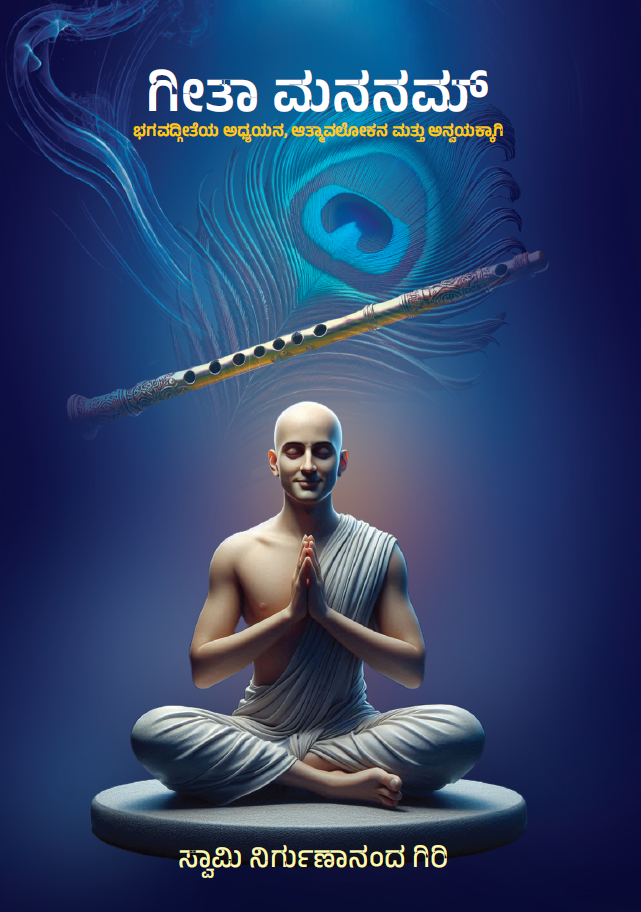
\includegraphics[width=\paperwidth,height=\paperheight]{./images/frontcover.png}%
    }%
}
    \begin{center}
        \vspace*{0.5cm}
            
        {\Huge
        %\textbf{\color{white}\fontsize{50}{60}\selectfont ಗೀತಾ ಮನನಂ}
		}
        %\textbf{\\ \small \color{white}ದೈನಂದಿನ ಸ್ಪೂರ್ತಿ ಹಾಗೂ ಆತ್ಮಾವಲೋಕನಕ್ಕಾಗಿ}    
        \vspace{1.0cm}
            
        
		
            
        \vfill
            
        
            
        \vspace{0.1cm}
        {\color{white}    
		%\textbf{{\Large \mananamfont ಸ್ವಾಮಿ ನಿರ್ಗುಣಾನಂದ ಗಿರಿ}}\\
		%{\normalsize Swami Nirgunananda Giri\\Rishikesh, India}
		}
    \end{center}
\end{titlepage}
\nopagecolor% Use this to restore the color pages to white
\begin{titlepage}
	%\pagecolor{pastelblue}
	%\AddToShipoutPictureBG*{%
    %\AtPageLowerLeft{%
    %    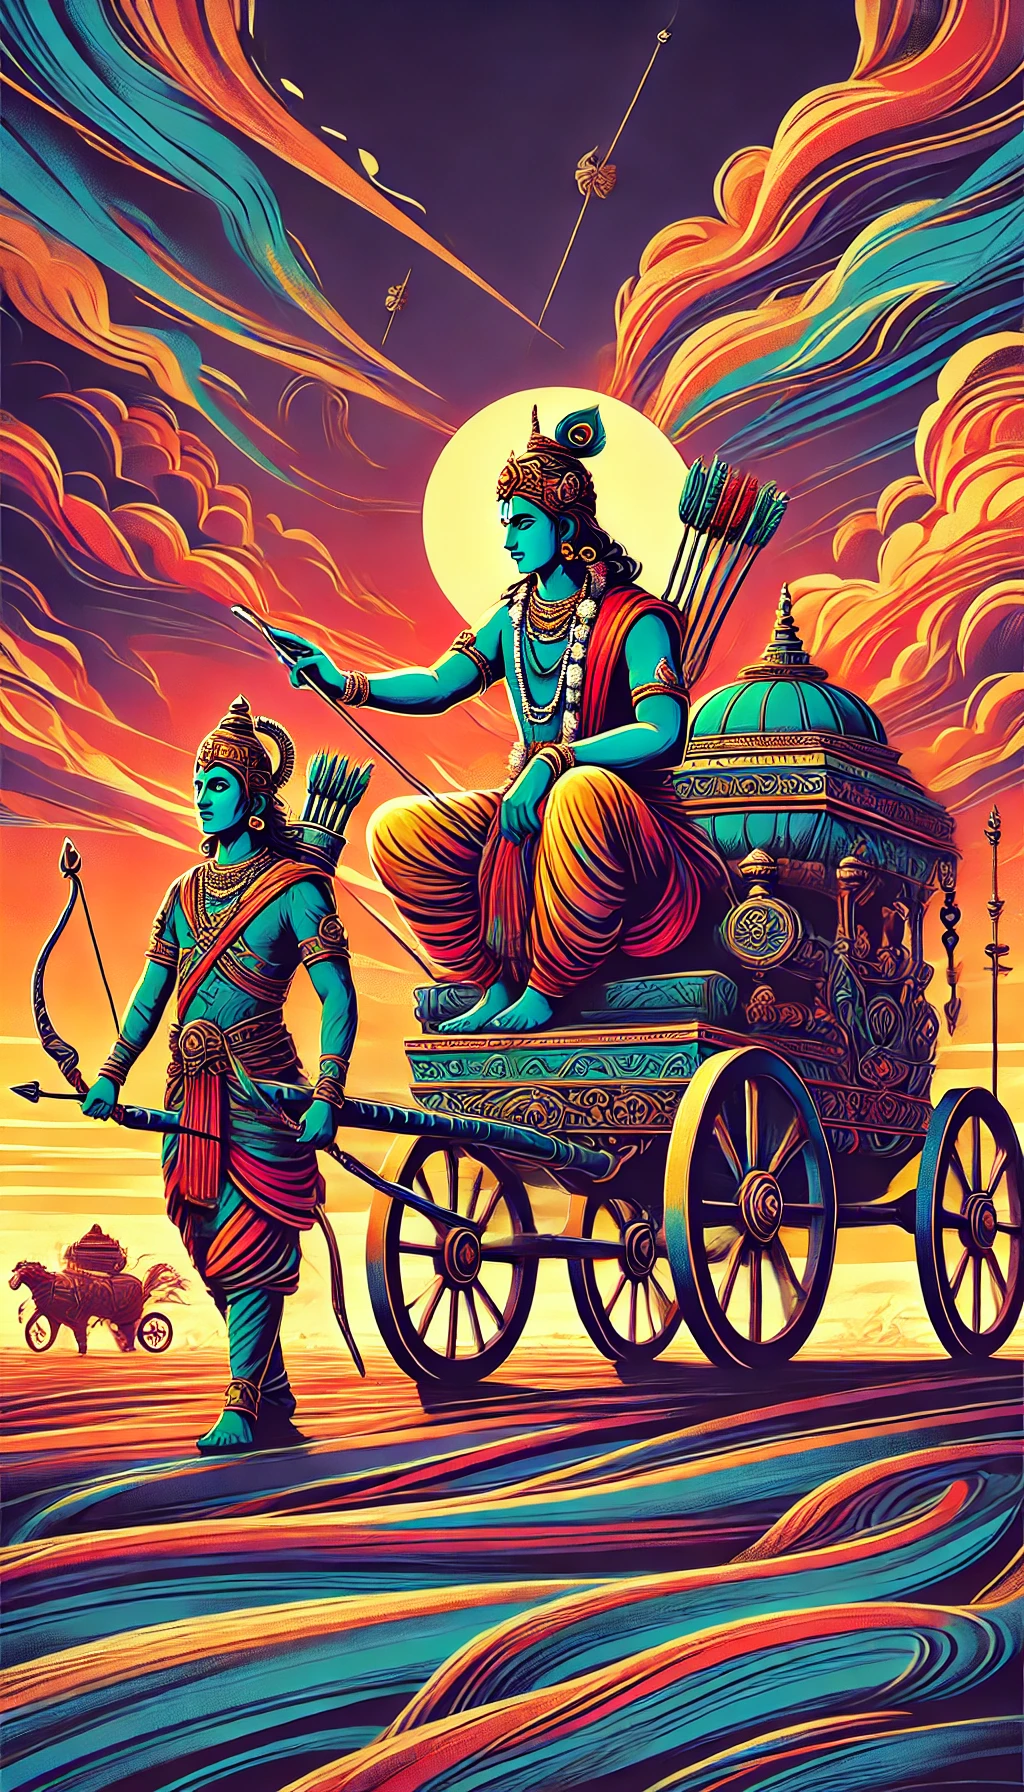
\includegraphics[width=\paperwidth,height=\paperheight]{./images/krishna4.jpg}%
    %}%
%}
    \begin{center}
        \vspace*{0.5cm}
            
        {\Huge
        \textbf{\color{blue}\fontsize{50}{60}\selectfont ಗೀತಾ ಮನನಂ}}
        \textbf{\\ \small \color{black}ದೈನಂದಿನ ಸ್ಪೂರ್ತಿ ಹಾಗೂ ಆತ್ಮಾವಲೋಕನಕ್ಕಾಗಿ}\\    
        \vspace{1.0cm}
		    \textbf{{\large \color{black} ಅಧ್ಯಾಯ ೫ ಕರ್ಮ ಸನ್ಯಾಸ ಯೋಗ}}\\		
        \vspace{6.0cm}
        \textbf{{\Large \color{blue}\mananamfont ಸ್ವಾಮಿ ನಿರ್ಗುಣಾನಂದ ಗಿರಿ}}\\    
        
		
            
        \vfill
            
        
            
        \vspace{0.1cm}
        {\color{black}    
		
		{{\large \color{blue}ಹೃಷೀಕೇಶ, ಉತ್ತರಾ ಖಂಡ}\\\normalsize ಭಾರತ}
        }
    \end{center}
\end{titlepage}
\nopagecolor% Use this to restore the color pages to white
%\maketitle

\thispagestyle{empty}
Copyright \textcopyright\ Swamy Nirgunanandagiri\\
\\
All rights reserved\\
\\
Edition - First, 2024\\
\vfill
Without written permission of the author it is forbidden to reproduce or adapt in any form or by any means any part of this  publication.\\
\\
Rishikesh, India\\
\newpage
\thispagestyle{empty}
\frontmatter

\doublespacing
\tableofcontents
\singlespacing
%\clearpage
%\newgeometry{margin=0pt} % Apply margin only for this page
%\thispagestyle{empty}
%\begin{center}
%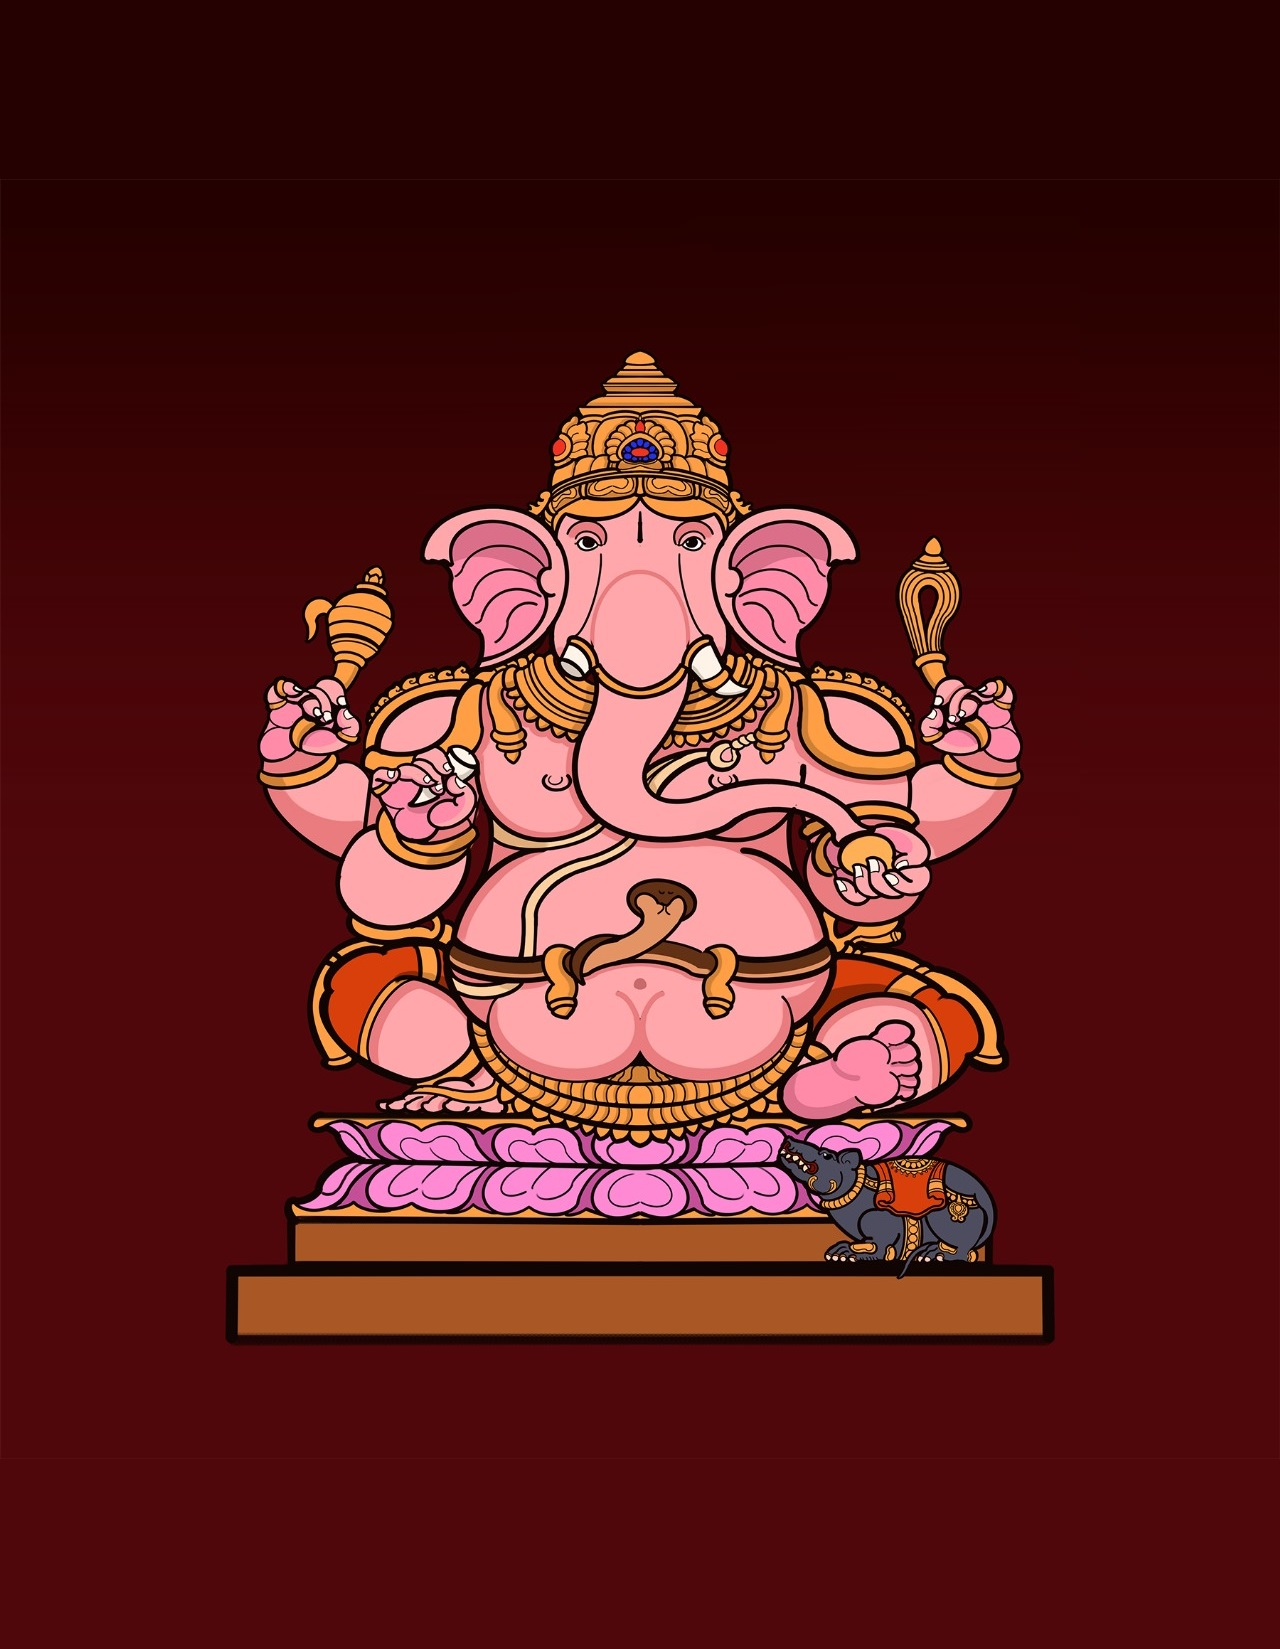
\includegraphics[width=0.9\textwidth, height=\paperheight, keepaspectratio]{./images/ganapa.jpg}
%\end{center}
%\restoregeometry % Restore original geometry settings
%\newpage

\clearpage
\newgeometry{margin=0pt} % Apply margin only for this page
\thispagestyle{empty}
%\begin{figure}
%\centering
%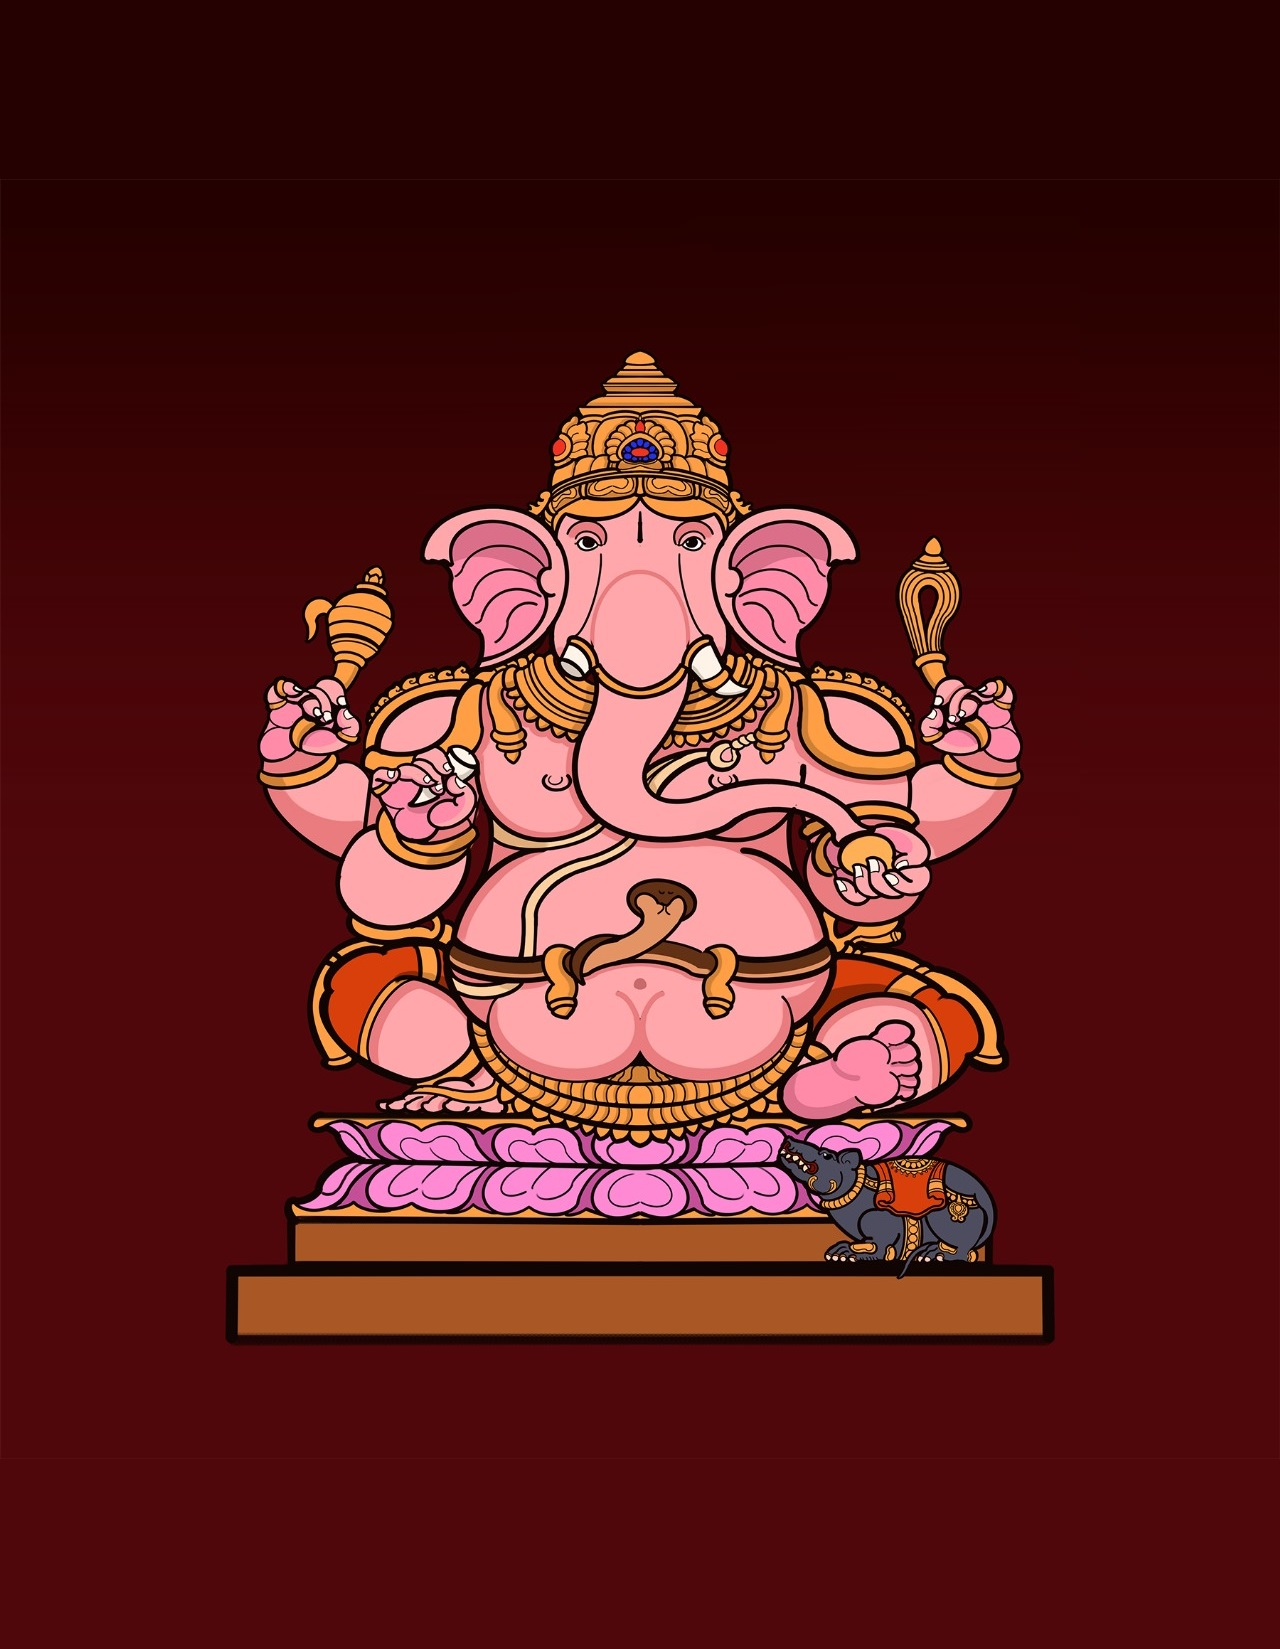
\includegraphics[width=0.9\textwidth, height=\paperheight, keepaspectratio]{./images/ganapa.jpg}
%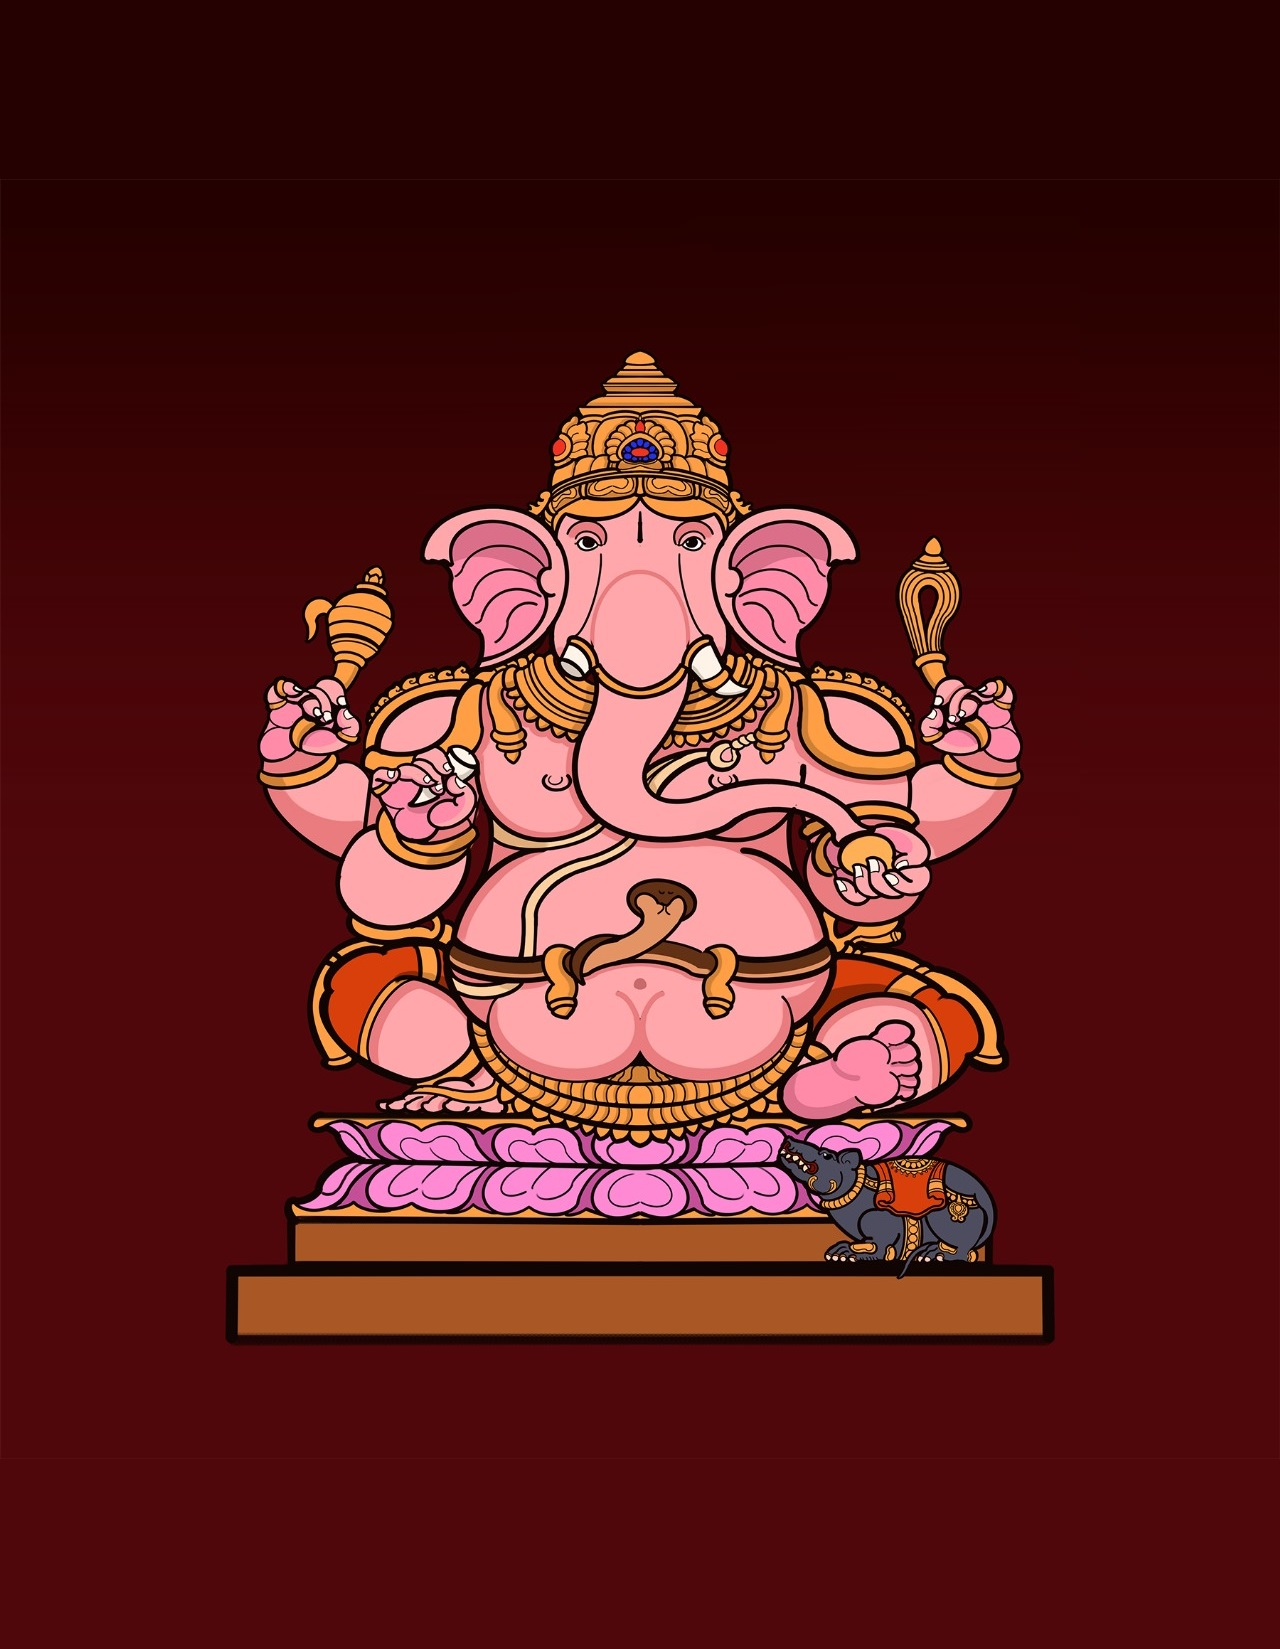
\includegraphics[width=\paperwidth, height=\paperheight]{./images/ganapa.jpg}
%\end{figure}
%\restoregeometry % Restore original geometry settings
%\newpage

\begin{figure}[h!]
    \centering
    \begin{overpic}[width=\paperwidth, height=\paperheight]{../images/001.jpg}
        \put(13,85){\color{white}\kanfont ಗಜಾನನಂ ಭೂತಗಣಾದಿ ಸೇವಿತಂ ಕಪಿತ್ಥ ಜಂಬೂಫಲಸಾರ ಭಕ್ಷಿತಮ್। }\put(10,82){\color{white}\kanfont ಉಮಾಸುತಂ ಶೋಕ ವಿನಾಶಕಾರಣಂ ನಮಾಮಿ ವಿಘ್ನೇಶ್ವರ ಪಾದಪಂಕಜಮ್॥ }
    \end{overpic}
    \caption{This is the standard figure caption below the image.}
    \label{fig:example}
\end{figure}

\restoregeometry

\thispagestyle{empty}
\thispagestyle{empty}
\pagestyle{fancy}


\chapter{\kanfont ಮುನ್ನುಡಿ}
\begin{center}
ದಿಶಂತು ಶಂ ಮೇ ಗುರುಪಾದಪಾಂಸವಃ ॥\\
\end{center}
\footnotesize \mananamtext{ಶ್ರಿ\!\char"0CD5ಮದ್ ಭಗವದ್ಗೀತೆಯು ಎಲ್ಲಾ ಧರ್ಮಗ್ರಂಥಗಳಲ್ಲಿ ಒಂದು ಅನನ್ಯ ಮತ್ತು ಸಾಟಿಯಿಲ್ಲದ ರತ್ನವಾಗಿದೆ.  ಇದು ಪರಿತ್ಯಾಗ ಮಾಡುವವರಿಗೆ ಮಾತ್ರವಲ್ಲದೆ ಲೌಕಿಕ ಜವಾಬ್ದಾರಿಗಳನ್ನು ಹೊತ್ತಿರುವವರಿಗೂ ಮಾರ್ಗದರ್ಶಿ ಬೆಳಕಾಗಿ ಕಾರ್ಯನಿರ್ವಹಿಸುತ್ತದೆ, ಆಧ್ಯಾತ್ಮಿಕದೊಂದಿಗೆ ಪ್ರಾಪಂಚಿಕತೆಯನ್ನು ಸಮತೋಲನಗೊಳಿಸಲು ಪ್ರಯತ್ನಿಸುತ್ತದೆ; ಇದು, ಅಜ್ಞಾನದಿಂದ ಅವರು (ಸಾಮಾನ್ಯ ಜನ) ತಮ್ಮನ್ನು ತಾವು,   ದೇಹ ಮತ್ತು ಮನಸ್ಸಿನ ವ್ಯವಹಾರಗಳ  ಜೊತೆ ಗುರುತಿಸಿಕೊಂಡಾಗ, ಅಂತಹ ವ್ಯವಹಾರಗಳ ಬಗ್ಗೆ ನಿಷ್ಪಕ್ಷಪಾತವಾಗಿರುವಂತೆ ಪ್ರತಿಪಾದಿಸುತ್ತದೆ.\\
ಜೀವನದಲ್ಲಿ ಒಬ್ಬರ ಕರ್ತವ್ಯಗಳನ್ನು ಸಾಧಿಸಲು, ಬಾಂಧವ್ಯದ ಅಥವಾ, ಮೋಹದ ಭಾವನೆ ಇರಬೇಕು ಎಂಬುದು ಒಂದು ತಪ್ಪು ಕಲ್ಪನೆ.  ಭಗವಾನ್ ಕೃಷ್ಣ, ಎಲ್ಲರಿಗಿಂತಲೂ  ದೊಡ್ಡ ಸಂಸಾರಿ ಹಾಗೂ, ಪರಿಪೂರ್ಣವಾದ ಮೋಹರಹಿತನಾದ ಅಸಂಸಾರಿ; ದಿವ್ಯವಾದ ಆನಂದದಲ್ಲಿ ನೆಲೆಗೊಂಡು, ಈ ಮೂರ್ತ, ಭೌತಿಕ ಜಗತ್ತಿನಲ್ಲಿ ಹೇಗೆ ಕಾರ್ಯನಿರ್ವಹಿಸಬೇಕು ಎಂಬುದನ್ನು ಅವನು ತನ್ನ ಕಾರ್ಯಗಳು, ಭಾವ ಮತ್ತು ಅವನು ಉಚ್ಛರಿಸುವ ಪ್ರತಿಯೊಂದೂ ಪರಮಪದದ  ಮೂಲಕ ಪ್ರದರ್ಶಿಸುತ್ತಾನೆ. ಆರಂಭದಲ್ಲಿ ‘ಸಂಘರ್ಷ ಮತ್ತು ಸವಾಲುಗಳಿಂದ ತುಂಬಿರುವ ಮಾರ್ಗ’ ಎಂದು ಕಂಡುಬoದರೂ ಸಹ, ಈ ಸ್ಥಿತಿಯನ್ನು ಸಾಧಿಸಲು (ದಿವ್ಯವಾದ ಆನಂದದಲ್ಲಿ ನೆಲೆಗೊಂಡು, ಈ ಮೂರ್ತ, ಭೌತಿಕ ಜಗತ್ತಿನಲ್ಲಿ  ಕಾರ್ಯನಿರ್ವಹಿಸುವುದು) ಸಮರ್ಥ ಶಿಕ್ಷಕರಿಂದ ಸರಿಯಾದ ಮಾರ್ಗದರ್ಶನದ ಅಗತ್ಯವಿದೆ. \\
ಈ ‘ನಿಪುಣ ಮಾರ್ಗದರ್ಶಿ ಕೈಪಿಡಿ’ಯಲ್ಲಿ, ಲೇಖಕರ ಆಳವಾದ ಒಳನೋಟದಿಂದ ಅಧ್ಯಾಯ 2 ರ 52-53 ಪದ್ಯಗಳಲ್ಲಿ ಸೂಚಿಸಿದಂತೆ: “ಶಿಕ್ಷಕರ ಮತ್ತು ಧರ್ಮಗ್ರಂಥಗಳ ಉದ್ದೇಶವು ನಮ್ಮನ್ನು ಭ್ರಮೆಯಿಂದ ಜಗ್ಗಿಸಿ, ಮುಕ್ತರನ್ನಾಗಿ ಮಾಡುವುದೇ ಆಗಿದೆ. ನಾವು ನಮ್ಮ ಲೌಕಿಕ ಚಿಂತನೆಯ ಮಾದರಿಗಳನ್ನು ಬಿಟ್ಟು, ಒಂದು ಉನ್ನತ ಸತ್ಯದಲ್ಲಿ (ಪಾರಮಾರ್ಥಿಕದಲ್ಲಿ) ಆಶ್ರಯ ಪಡೆಯಲು ಪ್ರಾರಂಭಿಸುತ್ತಿದ್ದಂತೆಯೇ, ಆಧ್ಯಾತ್ಮಿಕ ಪ್ರಯಾಣದ ಒಂದು ಭಾಗವಾದ ಗೊಂದಲಗಳು ಮತ್ತು ಸವಾಲುಗಳು ಏಳುತ್ತವೆ; ಆದರೆ, ನಾವು ಹೀಗೆ ಈ ಹಾದಿಯಲ್ಲಿ ಪ್ರಗತಿ ಹೊಂದುತ್ತಿದ್ದಂತೆ, ಸ್ಪಷ್ಟತೆ ಪಡೆಯಲು ಪ್ರಾರಂಭಿಸುತ್ತೇವೆ”.\\
ಈ ಪುಸ್ತಕವು ಲೇಖಕರ ಕ್ರಾಂತಿಕಾರಿ ಚಿಂತನೆಗಳ ಮೂಲಕ ಓದುಗರನ್ನು ದೇಹದಿಂದ, ಮನಸ್ಸಿಗೆ ಮತ್ತು ಮನಸ್ಸಿನಿಂದ ಪ್ರಜ್ಞೆಗೆ (ಚೈತನ್ಯಕ್ಕೆ), ಒಬ್ಬರ ಅಸ್ತಿತ್ವದ ಪದರಗಳನ್ನು ಭೇದಿಸುವಂತೆ ಮಾಡುತ್ತದೆ. \\
ಪ್ರತಿ ವಿಭಾಗದಲ್ಲಿ, ‘ಮನನಂ’ ಶೀರ್ಷಿಕೆಯಡಿಯಲ್ಲಿರುವ ಆತ್ಮಾವಲೋಕನದ ಪ್ರಶ್ನೆಗಳು, ಸ್ವಯಂ ಸಮಾಧಾನ ಮತ್ತು ಆತ್ಮವಂಚನೆಯಲ್ಲಿ (ಆತ್ಮ ಪ್ರವಂಚನ) ತೊಡಗಿರುವವರಿಗೆ ಯಾವುದೇ ವಿರಾಮ ನೀಡುವುದಿಲ್ಲ ಮತ್ತು ಪ್ರಾಮಾಣಿಕವಾದ ಸ್ವಯಂ ಮೌಲ್ಯಮಾಪನ ಮಾಡಲು ಅವರಿಗೆ ಸವಾಲು ಒಡ್ಡುತ್ತವೆ .  ಮತ್ತೊಂದೆಡೆ, ‘ಸ್ಫೂರ್ತಿ’ಯ ಅಡಿಯಲ್ಲಿರುವ ಪದಗಳು, ಪ್ರಯಾಸಕರ ಮತ್ತು ಗೊಂದಲಮಯ ಆಧ್ಯಾತ್ಮಿಕ ಮಾರ್ಗವನ್ನು ತುಲನಾತ್ಮಕವಾಗಿ ಸುಲಭಗೊಳಿಸಿ, ಸಕಾರಾತ್ಮಕತೆಯ ಒಂದು, ಅಕ್ಷಯವಾದ ಮೂಲವಾಗಿ ಕಾರ್ಯನಿರ್ವಹಿಸುತ್ತವೆ.\\
ಈ ಕೈಪಿಡಿಯು, ಆಕಾಂಕ್ಷಿಗಳಿಗೆ ಜೀವನದ ವಿವಿಧ ಸಮಸ್ಯೆಗಳಿಗೆ ಪರಿಹಾರವನ್ನು ಕಂಡುಕೊಳ್ಳಲು ಸಾಕಷ್ಟು ಸಮಾಧಾನಗಳನ್ನು  ನೀಡುತ್ತದೆ, ಆದರೆ ಬಾಹ್ಯವಾಗಿ ಅಲ್ಲ, ಆಂತರಿಕವಾಗಿ.\\
ಈ ಪುಸ್ತಕದ ವಿಷಯವು, ‘ಮಾನವ ಮನೋವಿಜ್ಞಾನ’ದ ಬಗ್ಗೆ ಲೇಖಕರ ಆಳವಾದ ತಿಳುವಳಿಕೆಯನ್ನು ತೋರಿಸುತ್ತದೆ, ಮೊದಲು ಸಕಾರಾತ್ಮಕ ಮಾನಸಿಕ ಸ್ಥಿತಿಯ ಕಡೆಗೆ ಮತ್ತು ನಂತರ ಅದನ್ನು ಮೀರಿ, ಆಂತರಿಕ ಶಾಶ್ವತವಾದ ಆತ್ಮದೆಡೆಗೆ, ಸರಳವಾಗಿ ಮುಂದುವರಿಯುತ್ತದೆ. \\
ಈ ಪುಸ್ತಕದ ಓದುಗರು ಈ ಪ್ರಯಾಣವನ್ನು ಪ್ರಾರಂಭಿಸಿದಾಗ, ಅವರು ಖಂಡಿತವಾಗಿಯೂ ಮಾನವ ಮನಸ್ಸಿನ ಕ್ಷೇತ್ರವನ್ನು ಮೀರುತ್ತಾರೆ ಮತ್ತು ಈ ಸ್ವರ್ಗೀಯ ಗೀತೆಯಾದ  ‘ಭಗವದ್ಗೀತೆ’ ಗಾಯಕನ ಕೃಪೆಯಿಂದ ‘ಅಧಿಷ್ಠಾನ ಚೈತನ್ಯಮ್’ (ಚೇತನಾತ್ಮಕದ ಅಂತಿಮ ಮೂಲತತ್ವ) ಅನ್ನು ತಲುಪುತ್ತಾರೆ. ಸಾಧಕರ ಅನುಕೂಲಕ್ಕಾಗಿ ತಮ್ಮ ಅಮೂಲ್ಯವಾದ ಆಲೋಚನೆಗಳನ್ನು ಲೇಖಿಸಿದ, ಸ್ವಾಮಿ ನಿರ್ಗುಣಾನಂದ ಗಿರಿ, ಇವರ ನಿಸ್ವಾರ್ಥ ಪ್ರಯತ್ನವನ್ನು,  ಸನಾತನ ಗುರುವಾದ, ಆ ಭಗವಂತ ಶ್ರೀಕೃಷ್ಣನು ಆಶೀರ್ವದಿಸಲಿ.\\\\
\begin{center}
ಮಂಗಳಂ ಸರ್ವಂ
\end{center}

{\kanBold ಸ್ವಾಮಿ ಸ್ವಾನಂದ ತೀರ್ಥ} \\
ಆಚಾರ್ಯ, ಕೈಲಾಸ್ ಆಶ್ರಮ\\
ಋಷಿಕೇಶ – ಉತ್ತರಖಂಡ\\
}
%\thispagestyle{empty}
\begin{onehalfspace}
\chapter{\kanfont ಪ್ರಸ್ತಾವನೆ}
\footnotesize \mananamtext{ನಾವೆಲ್ಲರೂ ಜೀವನದ ಹೋರಾಟಗಳನ್ನು ಎದುರಿಸಲೇಬೇಕು. ಕುರುಕ್ಷೇತ್ರ ಯುದ್ಧದಲ್ಲಿ ಶ್ರೀ ಕೃಷ್ಣ ಪರಮಾತ್ಮನು, ತನ್ನ ವೇದನಾಯುಕ್ತ ಶಿಷ್ಯ ಅರ್ಜುನನಿಗೆ, ಪ್ರಾಪಂಚಿಕತೆಯಲ್ಲಿಯೂ ಅಧ್ಯಾತ್ಮಿಕತೆಯನ್ನು ಆಚರಣೆಗೆ ತರುವಂತಹ, ಸಂಕ್ಷಿಪ್ತ ಹಾಗೂ ಪ್ರಾಯೋಗಿಕವಾದ,  ಅತೀ ಪವಿತ್ರವಾದ ಬೋಧನೆಗಳನ್ನು ಕೊಟ್ಟಿದ್ದಾನೆ. ಈ ಶ್ರೇಷ್ಠವಾದ ಉಪನಿಷತ್ತುಗಳ ಸತ್ವಗಳನ್ನೊಳಗೊಂಡ  ಬೋಧನೆಗಳನ್ನು ಪವಿತ್ರವಾದ, ‘ಭಗವದ್ಗೀತ, ಒಂದು ಪವಿತ್ರ ಗಾನ’ ದ ಸ್ವರೂಪದಲ್ಲಿ, ಋಷಿ ವೇದವ್ಯಾಸರು ನಮಗೆ ನೀಡಿರುವ ಅಸೀಮವಾದ ಕೊಡುಗೆ. \\
 ಅರ್ಜುನನು ಇದ್ದ ಪರಿಸ್ಥಿತಿಗೂ, ನಾವು ಇರುವ ಪರಿಸ್ಥಿತಿ ಮತ್ತು ಸಂಘರ್ಷಗಳಿಗೂ ವ್ಯತ್ಯಾಸಗಳಿರಬಹುದು. ಆದರೆ, ಗೀತೆಯ ಸಾರ್ವತ್ರಿಕ ಉಪದೇಶಗಳು ಸತ್ಯಾನ್ವೇಷಣೆ ಮಾಡಲು ಬಯಸುವ ಪ್ರತಿಯೊಬ್ಬನಿಗೂ ಆತ್ಮೋನ್ನತಿ  ಮತ್ತು ಅಧ್ಯಾತ್ಮಿಕ ಪ್ರಗತಿ ಸಾಧಿಸಲು ಬೇಕಾಗುವ ಮಾದರಿಯಾಗಿದೆ.\\
 ಭಗವದ್ಗೀತೆಯ ಉಪದೇಶಗಳು ಕೇವಲ ಆಧ್ಯಾತ್ಮಿಕ ಅನ್ವೇಷಣೆ ಮಾಡುವವರಿಗೆ ಸಮರ್ಪಿತವಾದದ್ದು ಮಾತ್ರವೇ ಅಲ್ಲ, ಜೀವನಕ್ಕೆ ಬೇಕಾಗುವ ಅತ್ಯಮೂಲ್ಯವಾದ ಕೈಪಿಡಿಯೂ ಆಗಿದೆ. ಯಾರು, ಕೆಲಸದಲ್ಲಿ ಮತ್ತು ಕೌಟುಂಬಿಕ ಜವಾಬ್ದಾರಿಗಳಲ್ಲಿ ಒತ್ತಡ ರಹಿತವಾಗಿ, ಸಮತೋಲನ ಮತ್ತು ಮಾನಸಿಕ ನೆಮ್ಮದಿ ಕಾಪಾಡಿಕೊಳ್ಳಲು  ಬಯಸುತ್ತಾರೋ ಅವರಿಗೆ ಈ ಬೋಧನೆಗಳು ಬಹಳ ಮಹತ್ವದ್ದಾಗಿರುತ್ತವೆ. \\
 ಅನೇಕ ಗುರುಗಳು ಮತ್ತು ವಿದ್ವಾಂಸರು ಈಗಾಗಲೇ ಮಾಡಿರುವಂತೆ ಈ ದಿನಚರಿ ಪುಸ್ತಕ ಮತ್ತು ನಿಯತಕಾಲಿಕವು, ಗೀತೆಯ ಬೋಧನೆಗಳನ್ನು ತಿಳಿಸುವ ಪ್ರಯತ್ನ ಅಥವಾ ವ್ಯಾಖ್ಯಾನ ಕೊಡುವುದಾಗಿಲ್ಲ. ಈ ಗೀತಾ ಮನನವು, ಬೋಧನೆಗಳ ಚಿಂತನೆ ಮಾಡುವುದು ಮತ್ತು ಅದನ್ನು ನಮ್ಮ ಸ್ವಂತದ್ದನ್ನಾಗಿ ಅಂದರೆ, ಜೀವನದಲ್ಲಿ ಅಳವಡಿಸಿಕೊಳ್ಳಲು ಸುಲಭವಾಗುವಂತೆ ಮಾಡಿಕೊಳ್ಳುವುದೇ ಆಗಿದೆ. ದೇವ ನಾಗರಿಯಲ್ಲಿರುವ `ಮನನ` ಎಂಬ ಪದವು ಆಗಲೇ ಕೇಳಿದ್ದನ್ನು ಅಥವಾ ಓದಿದ್ದನ್ನು ಚಿಂತನೆ ಮಾಡುವ ಕಾರ್ಯವಿಧಾನವನ್ನು ಅನ್ವಯಿಸುವುದಾಗಿದೆ.\\
 ಈ ದಿನಚರಿ ಪುಸ್ತಕವನ್ನು ನೀವು, ನಿಮ್ಮ ಮನಸ್ಸಿನ ಇಂಗಿತವನ್ನು ಸ್ವತಂತ್ರವಾಗಿ ವ್ಯಕ್ತಪಡಿಸಲು  ಮತ್ತು ನಿಮ್ಮ ಜೀವನದಲ್ಲಿ ಅಳವಡಿಸಿಕೊಳ್ಳಲು ಅವಕಾಶ ಮಾಡಿಕೊಡುವ ಸಲುವಾಗಿ  ರೂಪಿಸಲಾಗಿದೆ. ಗೀತೆಯಲ್ಲಿರುವ ಶ್ಲೋಕಗಳ ಆಧಾರದ ಮೇಲೆ ರಚಿಸಲಾಗಿರುವ ಈ ಪ್ರಶ್ನೆಗಳು, ಆಯಾ ಬೋಧನೆಗಳ ಸನ್ನಿವೇಶಕ್ಕೆ ತಕ್ಕಂತೆ, ನಿಮ್ಮ ವೈಯಕ್ತಿಕ ಅರ್ಥಗಳನ್ನು ಹುಡುಕಲು ಮತ್ತು ಅದರಿಂದ ಜೀವನದ ಸಂದರ್ಭದೊಳಗೆ ಅಪಾರ ಸ್ಪಷ್ಟನೆ ದೊರಕಿಸಲು ಸಹಾಯಕವಾಗುವಂತೆ ರೂಪಿಸಲಾಗಿದೆ.\\
 ಶ್ರಿ\!\char"0CD5ಕೃಷ್ಣ ಪರಮಾತ್ಮನು  ಅರ್ಜುನನಿಗೆ ಧಾರ್ಮಿಕ ಯುದ್ಧವನ್ನು ಮಾಡಲು ಪ್ರೇರೇಪಿಸಿದಂತೆ, ನಿಮ್ಮ ಜೀವನದ ದಿನನಿತ್ಯದ ಕರ್ತವ್ಯಗಳನ್ನು ಈ “ಗೀತಾ ಮನನಮ್ “ ಮೂಲಕ  ಸಮರ್ಪಕವಾಗಿ ನಿರ್ವಹಿಸಲು,  ಆ ಭಗವಂತ ನಿಮ್ಮನ್ನೂ ಪ್ರೇರೇಪಿಸುತ್ತಾನೆ ಎಂದು ನಂಬುತ್ತೇನೆ. ನಿಮ್ಮ ಅಂತರಂಗದ ಶಾಂತಿ, ವೈಯಕ್ತಿಕ ಪ್ರಗತಿಯನ್ನು ನಿರ್ಲಕ್ಷಿಸದೇ, ನಿಮ್ಮ ಕರ್ತವ್ಯಗಳನ್ನು ಕುಶಲತೆಯಿಂದ ಯಶಸ್ವಿಯಾಗಿ ನಿರ್ವಹಿಸುತ್ತಾ  ಮತ್ತು ನಿಶ್ಚಲವಾಗಿ ದೈವತ್ವದಲ್ಲಿ ಮನಸನ್ನಿಡುವುದೇ, ಈ ದಿವ್ಯವಾದ ಗೀತೆಯ ನಿರಂತರ ಉದ್ದೇಶ.\\
ನಾನು ಈ ಪುಸ್ತಕದಲ್ಲಿ ಬಳಸಿರುವ ಚಿತ್ರಕಲೆ ಮತ್ತು ರೇಖಾಚಿತ್ರಗಳಿಗಾಗಿ ಶ್ರಿ\!\char"0CD5ಯುತ ಕೆ.ಎಂ.ಶೇಷಗಿರಿ ಅವರಿಗೆ ಧನ್ಯವಾದಗಳನ್ನು ಸಲ್ಲಿಸುತ್ತೇನೆ. ನನ್ನ ಗೀತಾ ತರಗತಿಯಲ್ಲಿ ಭಾಗವಹಿಸಿದ್ದ ಅನೇಕ ವಿದ್ಯಾರ್ಥಿಗಳು ಶ್ಲೋಕಗಳ ಭಾಷಾಂತರ, ತಿದ್ದುವಿಕೆ, ಸಂಪಾದನೆ, ವಿನ್ಯಾಸ ಮತ್ತು ಮುದ್ರಣ ಪ್ರಕ್ರಿಯೆಯನ್ನು ಗಮನಿಸುವಲ್ಲಿ ತೊಡಗಿಸಿಕೊಂಡಿದ್ದಾರೆ. ಈ ಗ್ರಂಥವನ್ನು ಓದುಗರ ಹಿತಾರ್ಥಕ್ಕಾಗಿ ಸಮರ್ಪಣೆಯಿಂದ ಮಾಡಿದ ಅವರ ತ್ಯಾಗಮಯ ಸೇವೆಗೆ ಭಗವಂತನ ಕೃಪೆ ಹಾಗು ನನ್ನ ಆಶೀರ್ವಾದಗಳು. \\\\
}
{
\kanBold{ಸ್ವಾಮಿ ನಿರ್ಗುಣಾನಂದ ಗಿರಿ}
}

\end{onehalfspace}
\mainmatter
%\centerline{\textbf{ಅಥ ಪ್ರಥಮೋऽಧ್ಯಾಯಃ ।}\\}
ಮೊಟ್ಟ ಮೊದಲನೆಯ ಶ್ಲೋಕವೇ ನಮಗೆ ಚಿಂತನೆ, ಮನನ ಪ್ರಾರಂಭಿಸಲು ಬೇಕಾಗುವ ಸೂಕ್ಷ್ಮವಾದ ಸಂದೇಶವನ್ನು ಕೊಡುತ್ತದೆ.\\
\slcol{ಧೃತರಾಷ್ಟ್ರ ಉವಾಚ ।\\
\index{ಧರ್ಮಕ್ಷೇತ್ರೇ ಕುರುಕ್ಷೇತ್ರೇ} ಸಮವೇತಾ ಯುಯುತ್ಸವಃ ।\\
ಮಾಮಕಾಃ ಪಾಂಡವಾಶ್ಚೈವ ಕಿಮಕುರ್ವತ ಸಂಜಯ ॥ 1 ॥}
\cquote{ಧೃತರಾಷ್ಟ್ರನು ಹೇಳಿದನು,\\
ಸಂಜಯನೇ, ಯುದ್ಧದ ಬಯಕೆಯಿಂದ ಧರ್ಮಭೂಮಿಯಾದ ಕುರುಕ್ಷೇತ್ರದಲ್ಲಿ ಕಲೆತ ನನ್ನ ಮಕ್ಕಳೂ ಪಾಂಡವರೂ ಏನು ಮಾಡಿದರು?\\}
\slcol{ಸಂಜಯ ಉವಾಚ ।\\
\index{ದೃಷ್ಟ್ವಾ ತು ಪಾಂಡವಾನೀಕಂ} ವ್ಯೂಢಂ ದುರ್ಯೋಧನಸ್ತದಾ ।\\
ಆಚಾರ್ಯಮುಪಸಂಗಮ್ಯ ರಾಜಾ ವಚನಮಬ್ರವೀತ್ ॥ 2 ॥}
\cquote{ಸಂಜಯನು ಹೇಳಿದನು,\\
ಪಾಂಡವರ ದಂಡು ಸಜ್ಜಾಗಿ ನಿಂತಿದ್ದುದನ್ನು ನೋಡಿದ ಅರಸನಾದ ದುರ್ಯೋಧನನು ಗುರುಗಳಾದ ದ್ರೋಣರ ಬಳಿಗೆ ಬಂದು ಹೀಗೆ ಹೇಳಿದನು. \\}
\slcol{\index{ಪಶ್ಯೈತಾಂ ಪಾಂಡುಪುತ್ರಾಣಾಮಾಚಾರ್ಯ} ಮಹತೀಂ ಚಮೂಮ್ ।\\
ವ್ಯೂಢಾಂ ದ್ರುಪದಪುತ್ರೇಣ ತವ ಶಿಷ್ಯೇಣ ಧೀಮತಾ ॥ 3 ॥}
\cquote{ಗುರುಗಳೇ, ದೃಪದರಾಜನ ಮಗ ನಿಮ್ಮ ಶಿಷ್ಯ, ಬುದ್ಧಿಶಾಲಿಯಾದ ದೃಷ್ಟದ್ಯುಮ್ನ ಪಾಂಡವರ ಈ ದೊಡ್ಡ ದಂಡನ್ನು ಸಜ್ಜುಗೊಳಿಸಿರುವುದನ್ನು ನೋಡಿರಿ.\\}
\slcol{\index{ಅತ್ರ ಶೂರಾ ಮಹೇಷ್ವಾಸಾ} ಭೀಮಾರ್ಜುನಸಮಾ ಯುಧಿ ।\\
ಯುಯುಧಾನೋ ವಿರಾಟಶ್ಚ ದ್ರುಪದಶ್ಚ ಮಹಾರಥಃ ॥ 4 ॥}

\newpage
\begin{mananam}{\kanfont ಮನನ ಶ್ಲೋಕ - }
{\footnotesize \mananamfont ನನ್ನ ಜೀವನದ ದೈನಂದಿನ ನಿತ್ಯಕರ್ಮದಲ್ಲಿ ಯಾವಾಗ ನನ್ನ ದೇಹವು, ಆಸೆ, ಕೋಪ, ಭಯ, ಮತ್ಸರ ಇತ್ಯಾದಿಗಳಲ್ಲಿ ಒಲವು ತೋರುವುದನ್ನು ಗುರುತಿಸಿತು, ಅವುಗಳನ್ನು ಸ್ವಾತಂತ್ರ್ಯವನ್ನು ಆಳವಾಗಿ ಪ್ರೇರೇಪಿಸುವ ನನ್ನನ್ನು ಪ್ರತಿಭಟಿಸುವಂತೆ ಮಾಡುವ ಮತ್ತು ಸನಾತನ ಗ್ರಂಥ ಮತ್ತು ಬೋಧಕರಿಂದ ಪಡೆದ ಜ್ಞಾನವನ್ನು ಯಾವ ಬಲವನ್ನು ಅನುಸರಿಸಿದೆ? ನನ್ನ ಹಂಬಲ ಮತ್ತು ಸಂಕಲ್ಪಗಳನ್ನು ತಳ್ಳಿಹಾಕುವ ನನ್ನ ದುರಭ್ಯಾಸಗಳು ಮತ್ತು ಅಪಾಯಕಾರಿ ನಡವಳಿಕೆಗಳಿಂದಾಗಿ ನನ್ನ ನಿತ್ಯ ಜೀವನದಲ್ಲಿ ಏನೇನು ಕಷ್ಟ ಪಡಬೇಕಾಯಿತು?}
\end{mananam}
\WritingHand\enspace\textbf{ಆತ್ಮ ವಿಮರ್ಶೆ}
\begin{inspiration}{\kanfont ಸ್ಪೂರ್ತಿ}
{\footnotesize \mananamfont ನಿನಗೆ ನೀನು ಸತ್ಯವಾಗಿರು ಮತ್ತು ನೀನು ಉನ್ನತಿಯತ್ತ ಬದಲಾಗುವೆ. ಜೀವನದಲ್ಲಿ ಜಾಣನಿಗೆ ಅವಶ್ಯಕವಾದುದು ಪಕ್ಷಪಾತ ರಹಿತ ಅವಲೋಕನ. ನಮ್ಮನ್ನು ನಾವು ಬದಲಾಯಿಸಿಕೊಳ್ಳಲು ಕೇವಲ ಬಯಕೆ ಇದ್ದರೆ ಮಾತ್ರ ಸಾಲದು. ಜ್ಞಾನಿಗಳ ಮಹತ್ವದ, ಉನ್ನತವಾದ ಬೋಧನೆಗಳಿಂದ ನಮ್ಮ ಯೋಚನೆಗಳು, ಮಾತುಗಳು ಮತ್ತು ಕೃತಿಗಳನ್ನು ತಹಬಂದಿಗೆ ತಂದು, ಪ್ರತಿದಿನವೂ ನಮ್ಮನ್ನು ನಾವು ಆತ್ಮ ವಿಮರ್ಶೆ ಮಾಡಿಕೊಳ್ಳಲೇಬೇಕು.}
\end{inspiration}
\newpage

\cquote{ಈ ದಂಡಿನಲ್ಲಿ ಹೋರಾಟದಲ್ಲಿ ಭೀಮಾರ್ಜುನರಿಗೆ ಸರಿ ಜೋಡಿಯಾದ ಶೂರರಾಗಿ ದೊಡ್ಡ ದೊಡ್ಡ ಬಿಲ್ಲುಗಳನ್ನು ಹಿಡಿದುಕೊಂಡು ಕಾದುವುದರಲ್ಲಿ ಕುಶಲರಾದ ಸಾತ್ಯಕಿ ವಿರಾಟರಿದ್ದಾರೆ. ಸಹಸ್ರ ಜನರೊಡನೆ ಏಕಾಂಗಿಯಾಗಿ ಹೋರಾಡಬಲ್ಲ ದ್ರುಪದನಿದ್ದಾನೆ.\\}
\slcol{\index{ಧೃಷ್ಟಕೇತುಶ್ಚೇಕಿತಾನಃ} ಕಾಶಿರಾಜಶ್ಚ ವೀರ್ಯವಾನ್ ।\\
ಪುರುಜಿತ್ಕುಂತಿಭೋಜಶ್ಚ ಶೈಬ್ಯಶ್ಚ ನರಪುಂಗವಃ ॥ 5 ॥}
\cquote{ದೃಷ್ಟಕೇತು, ಚೀಕಿತಾನ, ವೀರನಾದ ಕಾಶಿರಾಜ, ಮತ್ತು ಮನುಷ್ಯರಲ್ಲಿ ಶ್ರೇಷ್ಠನಾದ ಶೈಭ್ಯ ಇವರೆಲ್ಲ ಇದ್ದಾರೆ. \\} 
\slcol{\index{ಯುಧಾಮನ್ಯುಶ್ಚ ವಿಕ್ರಾಂತ} ಉತ್ತಮೌಜಾಶ್ಚ ವೀರ್ಯವಾನ್ ।\\
ಸೌಭದ್ರೋ ದ್ರೌಪದೇಯಾಶ್ಚ ಸರ್ವ ಏವ ಮಹಾರಥಾಃ ॥ 6 ॥}
\cquote{ಬಲಶಾಲಿಯಾದ ಯುಧಾಮನ್ಯು, ವೀರನಾದ ಉತ್ತಮೌಜ, ಸುಭದ್ರೆಯ ಮಗ ಅಭಿಮನ್ಯು ಮತ್ತು ದ್ರೌಪದಿಯ ಮಕ್ಕಳು ಇದ್ದಾರೆ. ಎಲ್ಲರೂ ಒಬ್ಬೊಬ್ಬರು ಹತ್ತು ಸಹಸ್ರ ಜನರೊಡನೆ ಹೋರಾಡಬಲ್ಲ ಮಹಾರುತರು. \\}
\slcol{\index{ಅಸ್ಮಾಕಂ ತು ವಿಶಿಷ್ಟಾ ಯೇ} ತಾನ್ನಿಬೋಧ ದ್ವಿಜೋತ್ತಮ ।\\
ನಾಯಕಾ ಮಮ ಸೈನ್ಯಸ್ಯ ಸಂಙ್ಞಾರ್ಥಂ ತಾನ್ಬ್ರವೀಮಿ ತೇ ॥ 7 ॥}
\cquote{ಬ್ರಾಹ್ಮಣ ಶ್ರೇಷ್ಠರೇ, ನಮ್ಮ ಕಡೆಯಲ್ಲಿರುವ ವೀರರನ್ನು ನೆನಪಿಗೆ ತಂದುಕೊಳ್ಳಿ. ತಮಗೆ ನೆನಪಾಗಲೆಂದು ಅವರ ಹೆಸರುಗಳನ್ನು ಹೇಳುತ್ತೇನೆ.\\} 
\slcol{\index{ಭವಾನ್ಭೀಷ್ಮಶ್ಚ ಕರ್ಣಶ್ಚ} ಕೃಪಶ್ಚ ಸಮಿತಿಂಜಯಃ ।\\
ಅಶ್ವತ್ಥಾಮಾ ವಿಕರ್ಣಶ್ಚ ಸೌಮದತ್ತಿಸ್ತಥೈವ ಚ ॥ 8 ॥}
\cquote{ತಾವು ಭೀಷ್ಮ ಕರ್ಣ ಜಯಶೀಲನಾದ ಕೃಪಾ, ಅಶ್ವತ್ಥಾಮ, ವಿಕರ್ಣ ಸೋಮದತ್ತನ ಮಗನಾದ ಭೂರಿಶ್ರವ ಮತ್ತು ಜಯದ್ರಥ. \\}
\slcol{\index{ಅನ್ಯೇ ಚ ಬಹವಃ} ಶೂರಾ ಮದರ್ಥೇ ತ್ಯಕ್ತಜೀವಿತಾಃ ।\\
ನಾನಾಶಸ್ತ್ರಪ್ರಹರಣಾಃ ಸರ್ವೇ ಯುದ್ಧವಿಶಾರದಾಃ ॥ 9 ॥}
\cquote{ಇನ್ನೂ ಅನೇಕ ಶೂರರು ನನಗಾಗಿ ಜೀವ ತೆರಲು ಸಿದ್ದರಾಗಿ ಇದ್ದಾರೆ. ಎಲ್ಲರೂ ಎಲ್ಲ ಬಗಯ ಆಯುಧಗಳನ್ನು ಉಪಯೋಗಿಸಬಲ್ಲವರು ಮತ್ತು ಯುದ್ಧದಲ್ಲಿ ಗಟ್ಟಿಗರು.\\}
\slcol{\index{ಅಪರ್ಯಾಪ್ತಂ ತದಸ್ಮಾಕಂ} ಬಲಂ ಭೀಷ್ಮಾಭಿರಕ್ಷಿತಮ್ ।\\
ಪರ್ಯಾಪ್ತಂ ತ್ವಿದಮೇತೇಷಾಂ ಬಲಂ ಭೀಮಾಭಿರಕ್ಷಿತಮ್ ॥ 10 ॥}
\cquote{ಭೀಷ್ಮರ ರಕ್ಷಣೆಗೆ ಒಳಪಟ್ಟಿರುವ ನಮ್ಮ ದೊಡ್ಡ ಆ ದಂಡು ಸಾಲದೇನೋ ಎನಿಸುತ್ತದೆ. ಭೀಮನ ರಕ್ಷಣೆಗೆ ಒಳಪಟ್ಟಿರುವ ಪಾಂಡವರ ಈ ಸೇನೆ ಸಾಕಷ್ಟು ಸಮರ್ಥವಾಗಿದೆ.\\}
\slcol{\index{ಅಯನೇಷು ಚ ಸರ್ವೇಷು} ಯಥಾಭಾಗಮವಸ್ಥಿತಾಃ ।\\
ಭೀಷ್ಮಮೇವಾಭಿರಕ್ಷಂತು ಭವಂತಃ ಸರ್ವ ಏವ ಹಿ ॥ 11 ॥}
\cquote{ನೀವೆಲ್ಲರೂ ದಂಡಿನ ಬೇರೆ ಬೇರೆ ಮಾರ್ಗಗಳಲ್ಲಿ ನಿಮ್ಮ ನಿಮ್ಮ ಪಾಲಿಗೆ ಬಂದ ಕಡೆ ಇದ್ದುಕೊಂಡು ಭೀಷ್ಮನನ್ನು ರಕ್ಷಿಸಿರಿ.\\}
\slcol{\index{ತಸ್ಯ ಸಂಜನಯನ್ಹರ್ಷಂ} ಕುರುವೃದ್ಧಃ ಪಿತಾಮಹಃ ।\\
ಸಿಂಹನಾದಂ ವಿನದ್ಯೋಚ್ಚೈಃ ಶಂಖಂ ದಧ್ಮೌ ಪ್ರತಾಪವಾನ್ ॥ 12 ॥}
\cquote{ಹೀಗೆಂದು ಹೇಳಿದ ದುರ್ಯೋಧನನಿಗೆ ಹರ್ಷ ಉಂಟಾಗುವಂತೆ ಆಗ ಕುರುವಂಶದ ಹಿರಿಯ ಕೌರವರ ಅಜ್ಜ, ಪರಾಕ್ರಮಶಾಲಿ ಭೀಷ್ಮನು ಗಟ್ಟಿಯಾಗಿ ಸಿಂಹನಾದ ಮಾಡಿ ಶಂಖವನ್ನು ಊದಿದನು.\\}
\slcol{\index{ತತಃ ಶಂಖಾಶ್ಚ ಭೇರ್ಯಶ್ಚ} ಪಣವಾನಕಗೋಮುಖಾಃ ।\\
ಸಹಸೈವಾಭ್ಯಹನ್ಯಂತ ಸ ಶಬ್ದಸ್ತುಮುಲೋऽಭವತ್ ॥ 13 ॥}
\cquote{ಆಮೇಲೆ ಒಮ್ಮೆಲೆ ಶಂಖಗಳು, ಭೇರಿಗಳು, ಮೃದಂಗಗಳು, ನಗಾಡಿಗಳು, ರಣ ಸಿಂಹಗಳು ಒಳಗಿದವು. ಆ ಗದ್ದಲವು ಎಲ್ಲೆಲ್ಲಿಯೂ ತುಂಬಿತು.\\}
\slcol{\index{ತತಃ ಶ್ವೇತೈರ್ಹಯೈರ್ಯುಕ್ತೇ} ಮಹತಿ ಸ್ಯಂದನೇ ಸ್ಥಿತೌ ।\\
ಮಾಧವಃ ಪಾಂಡವಶ್ಚೈವ ದಿವ್ಯೌ ಶಂಖೌ ಪ್ರದಘ್ಮತುಃ ॥ 14 ॥}
\cquote{ಆಮೇಲೆ ಬಿಳಿ ಕುದುರೆಯನ್ನು ಹೂಡಿದ ದೊಡ್ಡ ತೇರಿನ ಮೇಲೆ ಕುಳಿತಿದ್ದ ಕೃಷ್ಣನೂ ಅರ್ಜುನನೂ ಹೆಸರುವಾಸಿಯಾದ ದಿವ್ಯವಾದ ತಮ್ಮ ಶಂಖಗಳನ್ನು ಊದಿದರು.\\}
\slcol{\index{ಪಾಂಚಜನ್ಯಂ ಹೃಷೀಕೇಶೋ} ದೇವದತ್ತಂ ಧನಂಜಯಃ ।\\
ಪೌಂಡ್ರಂ ದಧ್ಮೌ ಮಹಾಶಂಖಂ ಭೀಮಕರ್ಮಾ ವೃಕೋದರಃ ॥ 15 ॥}
\cquote{ಕೃಷ್ಣನು ಪಾಂಚಜನ್ಯವನ್ನೂ ಅರ್ಜುನನ್ನು ದೇವದತ್ತವನ್ನೂ, ಶತ್ರುಗಳನ್ನು ಎದೆಗೂಡಿಸುವ ಭೀಮನು ಪೌಂಡ್ರವೆಂಬ ದೊಡ್ಡ ಶಂಖವನ್ನು ಓದಿದನು.\\}
\slcol{\index{ಅನಂತವಿಜಯಂ ರಾಜಾ} ಕುಂತೀಪುತ್ರೋ ಯುಧಿಷ್ಠಿರಃ ।\\
ನಕುಲಃ ಸಹದೇವಶ್ಚ ಸುಘೋಷಮಣಿಪುಷ್ಪಕೌ ॥ 16 ॥}
\cquote{ಕುಂತಿಯ ಹಿರಿಯ ಮಗ, ಅರಸನಾದ ಧರ್ಮರಾಯನು ಅನಂತ ವಿಜಯವನ್ನೂ ನಕುಲನೂ ಸುಘೋಷವನ್ನೂ ಸಹದೇವನು ಮಣಿಪುಷ್ಪಕವನ್ನೂ ಊದಿದರು. \\}
\slcol{\index{ಕಾಶ್ಯಶ್ಚ ಪರಮೇಷ್ವಾಸಃ} ಶಿಖಂಡೀ ಚ ಮಹಾರಥಃ ।\\
ಧೃಷ್ಟದ್ಯುಮ್ನೋ ವಿರಾಟಶ್ಚ ಸಾತ್ಯಕಿಶ್ಚಾಪರಾಜಿತಃ ॥ 17 ॥\\
\index{ದ್ರುಪದೋ ದ್ರೌಪದೇಯಾಶ್ಚ} ಸರ್ವಶಃ ಪೃಥಿವೀಪತೇ ।\\
ಸೌಭದ್ರಶ್ಚ ಮಹಾಬಾಹುಃ ಶಂಖಾಂದಧ್ಮುಃ ಪೃಥಕ್ಪೃಥಕ್ ॥ 18 ॥}
\cquote{ಓ ಧೃತರಾಷ್ಟ್ರ ಕೇಳು, ಹಿರಿಯ ಬಿಲ್ಲೋಜ ಕಾಶಿರಾಜ, ಮಹಾರಥನಾದ ಶಿಖಂಡಿ, ಧೃಷ್ಟದ್ಯುಮ್ನ,  ವಿರಾಟ, ಸೋಲರಿಯದ ಸಾತ್ಯಕಿ, ದ್ರುಪದ, ದ್ರೌಪದಿಯ ಮಕ್ಕಳು, ಮಹಾಬಾಹುವಾದ ಅಭಿಮನ್ಯು ಹೀಗೆ ಎಲ್ಲರೂ ತಮ್ಮ ತಮ್ಮ ಶಂಖಗಳನ್ನು ಊದಿದರು.\\}
\slcol{\index{ಸ ಘೋಷೋ ಧಾರ್ತರಾಷ್ಟ್ರಾಣಾಂ} ಹೃದಯಾನಿ ವ್ಯದಾರಯತ್ ।\\
ನಭಶ್ಚ ಪೃಥಿವೀಂ ಚೈವ ತುಮುಲೋ ವ್ಯನುನಾದಯನ್ ॥ 19 ॥}
\cquote{ಆ ಗದ್ದಲವು ಭೂಮಿಯಲ್ಲಿಯೂ ಆಕಾಶದಲ್ಲಿಯೂ ತುಂಬಿ ಪ್ರತಿಧ್ವನಿಯನ್ನು ಹಬ್ಬಿಸಿ ಕೌರವರ ಎದೆ ಬಿರಿಯುವಂತೆ ಮಾಡಿತು.\\}
\slcol{\index{ಅಥ ವ್ಯವಸ್ಥಿತಾಂದೃಷ್ಟ್ವಾ} ಧಾರ್ತರಾಷ್ಟ್ರಾನ್ಕಪಿಧ್ವಜಃ ।\\
ಪ್ರವೃತ್ತೇ ಶಸ್ತ್ರಸಂಪಾತೇ ಧನುರುದ್ಯಮ್ಯ ಪಾಂಡವಃ ॥ 20 ॥\\
\index{ಹೃಷೀಕೇಶಂ ತದಾ} ವಾಕ್ಯಮಿದಮಾಹ ಮಹೀಪತೇ ।}
\cquote{ಓ ಧೃತರಾಷ್ಟ್ರ, ಸಜ್ಜಾಗಿ ಎದುರಿಗೆ ನಿಂತಿರುವ ಕೌರವರನ್ನು ನೋಡಿ ಕಪಿಧ್ವಜನಾದ ಅರ್ಜುನನು ಹೊಡೆದಾಟಕ್ಕೆ ಮೊದಲು ಮಾಡಬೇಕಾದ ಆ ಸಮಯದಲ್ಲಿ ಗಾಂಡೀವವನ್ನು ಕೈಗೆ ತೆಗೆದುಕೊಂಡು ಕೃಷ್ಣನನ್ನು ಕುರಿತು ಈ ಮಾತನ್ನು ಹೇಳಿದನು.\\}
\slcol{ಅರ್ಜುನ ಉವಾಚ ।\\
ಸೇನಯೋರುಭಯೋರ್ಮಧ್ಯೇ ರಥಂ ಸ್ಥಾಪಯ ಮೇऽಚ್ಯುತ ॥ 21 ॥}
\cquote{ಅರ್ಜುನನ್ನು ಹೇಳಿದನು, ಕೃಷ್ಣ, ಎರಡು ದಂಡುಗಳ ನಡುವೆ ನನ್ನ ರಥವನ್ನು ನಿಲ್ಲಿಸು.\\}
\slcol{\index{ಯಾವದೇತಾನ್ನಿರೀಕ್ಷೇऽಹಂ} ಯೋದ್ಧುಕಾಮಾನವಸ್ಥಿತಾನ್ ।\\
ಕೈರ್ಮಯಾ ಸಹ ಯೋದ್ಧವ್ಯಮಸ್ಮಿನ್ರಣಸಮುದ್ಯಮೇ ॥ 22 ॥}
\cquote{ಕಾದಬೇಕೆಂದು ನಿಂತಿರುವವರನ್ನು, ಈ ಯುದ್ಧದಲ್ಲಿ ನಾನು ಯಾರೊಡನೆ ಕಾದಬೇಕಾಗಿದೆ ಎಂಬುದನ್ನು ಒಮ್ಮೆ ನೋಡುತ್ತೇನೆ.\\}
\slcol{\index{ಯೋತ್ಸ್ಯಮಾನಾನವೇಕ್ಷೇऽಹಂ} ಯ ಏತೇऽತ್ರ ಸಮಾಗತಾಃ ।\\
ಧಾರ್ತರಾಷ್ಟ್ರಸ್ಯ ದುರ್ಬುದ್ಧೇರ್ಯುದ್ಧೇ ಪ್ರಿಯಚಿಕೀರ್ಷವಃ ॥ 23 ॥}
\cquote{ದುರ್ಬುದ್ಧಿಯ ದುರ್ಯೋಧನನಿಗೆ ಈ ಯುದ್ಧದಲ್ಲಿ ನೆರವಾಗಬೇಕೆಂದು ಕಾದುವುದಕ್ಕಾಗಿ ಯಾರು ಯಾರು ಇಲ್ಲಿಗೆ ಬಂದಿರುತ್ತಾರೆ ಎಂಬುದನ್ನು ನಾನೊಮ್ಮೆ ನೋಡುತ್ತೇನೆ.\\}
\slcol{ಸಂಜಯ ಉವಾಚ ।\\
\index{ಏವಮುಕ್ತೋ ಹೃಷೀಕೇಶೋ} ಗುಡಾಕೇಶೇನ ಭಾರತ ।\\
ಸೇನಯೋರುಭಯೋರ್ಮಧ್ಯೇ ಸ್ಥಾಪಯಿತ್ವಾ ರಥೋತ್ತಮಮ್ ॥ 24 ॥\\
\index{ಭೀಷ್ಮದ್ರೋಣಪ್ರಮುಖತಃ} ಸರ್ವೇಷಾಂ ಚ ಮಹೀಕ್ಷಿತಾಮ್ ।\\
ಉವಾಚ ಪಾರ್ಥ ಪಶ್ಯೈತಾನ್ಸಮವೇತಾನ್ಕುರೂನಿತಿ ॥ 25 ॥}
\cquote{ಸಂಜಯನು ಹೇಳಿದನು,\\
ಧೃತರಾಷ್ಟ್ರನೇ, ಅರ್ಜುನನು ಹೀಗೆ ಹೇಳಿದಾಗ ಕೃಷ್ಣನು ಭೀಷ್ಮ ದ್ರೋಣರ ಮತ್ತು ಎಲ್ಲಾ ಅರಸರ ಎದುರಿಗೆ ಎರಡು ದಂಡುಗಳ ನಡುವೆ ರಥವನ್ನು ನಿಲ್ಲಿಸಿ ‘ಅರ್ಜುನನೇ ಇಲ್ಲಿ ನೆರೆದಿರುವರನ್ನು ನೋಡು’ ಎಂದು ಹೇಳಿದನು.\\}
\slcol{\index{ತತ್ರಾಪಶ್ಯತ್ಸ್ಥಿತಾನ್ಪಾರ್ಥಃ} ಪಿತೂನಥ ಪಿತಾಮಹಾನ್ ।\\
ಆಚಾರ್ಯಾನ್ಮಾತುಲಾನ್ಭ್ರಾತೂನ್ಪುತ್ರಾನ್ಪೌತ್ರಾನ್ಸಖೀಂಸ್ತಥಾ ॥ 26 ॥}
\cquote{ಅರ್ಜುನು ಅಲ್ಲಿ ನಿಂತಿರುವ ಪಿತೃತುಲ್ಯರು, ಅಜ್ಜಂದಿರು, ಗುರುಗಳು, ಸೋದರ ಮಾವಂದಿರು, ಅಣ್ಣತಮ್ಮಂದಿರು, ಮಕ್ಕಳು, ಮೊಮ್ಮಕ್ಕಳು, ಜೊತೆಗಾರರು, ಮಾವಂದಿರು, ಸ್ನೇಹಿತರು- ಹೀಗೆ ಎಲ್ಲ ಬಗೆಯ ಬಂಧುಗಳನ್ನು ಎರಡು ಕಡೆಯ ದಂಡಿನಲ್ಲಿ ಕಂಡನು.\\}
\slcol{\index{ಶ್ವಶುರಾನ್ಸುಹೃದಶ್ಚೈವ} ಸೇನಯೋರುಭಯೋರಪಿ ।\\
ತಾನ್ಸಮೀಕ್ಷ್ಯ ಸ ಕೌಂತೇಯಃ ಸರ್ವಾನ್ಬಂಧೂನವಸ್ಥಿತಾನ್ ॥ 27 ॥}
\cquote{ಹೀಗೆ ಅಲ್ಲಿ ನೆರೆದಿರುವ ಬಂಧುಗಳನ್ನೆಲ್ಲ ನೋಡಿ ಅರ್ಜುನನು ತುಂಬಾ ಕನಿಕರಗೊಂಡು ವಿಷಾದದಿಂದ ಈ ಮಾತನ್ನು ಹೇಳಿದನು.\\}
\slcol{\index{ಕೃಪಯಾ ಪರಯಾವಿಷ್ಟೋ} ವಿಷೀದನ್ನಿದಮಬ್ರವೀತ್ ।\\
ಅರ್ಜುನ ಉವಾಚ ।\\
ದೃಷ್ಟ್ವೇಮಂ ಸ್ವಜನಂ ಕೃಷ್ಣ ಯುಯುತ್ಸುಂ ಸಮುಪಸ್ಥಿತಮ್ ॥ 28 ॥\\
\index{ಸೀದಂತಿ ಮಮ ಗಾತ್ರಾಣಿ} ಮುಖಂ ಚ ಪರಿಶುಷ್ಯತಿ ।\\
ವೇಪಥುಶ್ಚ ಶರೀರೇ ಮೇ ರೋಮಹರ್ಷಶ್ಚ ಜಾಯತೇ ॥ 29 ॥}
\cquote{ಅರ್ಜುನನು ಹೇಳಿದನು,\\
ಕೃಷ್ಣ, ಕಾದುವುದಕೆಂದು ನೆರೆದಿರುವ ಈ ನನ್ನವರನ್ನು ನೋಡಿ ನನ್ನ ಅವಯವಗಳು ಸೊರುಗುತ್ತಿವೆ. ಬಾಯಿ ಒಣಗುತ್ತಿದೆ. ನನ್ನ ಮೈಯಲ್ಲಿ ನಡುಕ ಮೂಡಿ ರೋಮ ನಿಗುರಿ ನಿಂತಿದೆ.\\}
\slcol{\index{ಗಾಂಡೀವಂ ಸ್ರಂಸತೇ} ಹಸ್ತಾತ್ತ್ವಕ್ಚೈವ ಪರಿದಹ್ಯತೇ ।\\
ನ ಚ ಶಕ್ನೋಮ್ಯವಸ್ಥಾತುಂ ಭ್ರಮತೀವ ಚ ಮೇ ಮನಃ ॥ 30 ॥}
\cquote{ಕೈಯಿಂದ ಗಾಂಡೀವ ಧನುಸ್ಸು ಕುಸಿಯುತ್ತಿದೆ. ಚರ್ಮವು ಸುಡುತ್ತಿದೆ. ನನಗೆ ನಿಲ್ಲುವುದಕ್ಕೂ ಆಗುವುದಿಲ್ಲ. ನನ್ನ ಮನಸ್ಸು ತಳಮಳಗೊಂಡಿದೆ.\\}
\slcol{\index{ನಿಮಿತ್ತಾನಿ ಚ ಪಶ್ಯಾಮಿ} ವಿಪರೀತಾನಿ ಕೇಶವ ।\\
ನ ಚ ಶ್ರೇಯೋऽನುಪಶ್ಯಾಮಿ ಹತ್ವಾ ಸ್ವಜನಮಾಹವೇ ॥ 31 ॥}
\cquote{ಕೃಷ್ಣ, ಕೆಟ್ಟ ಅಪಶಕುನಗಳನ್ನು ಕಾಣುತ್ತಿದ್ದೇನೆ. ಯುದ್ಧದಲ್ಲಿ ನನ್ನವರನ್ನು ಕೊಂದರೆ ಒಳ್ಳೆಯದಾದೀತೆಂದು ನನಗೆ ಅನ್ನಿಸುವುದಿಲ್ಲ.\\}
\slcol{\index{ನ ಕಾಂಕ್ಷೇ ವಿಜಯಂ ಕೃಷ್ಣ} ನ ಚ ರಾಜ್ಯಂ ಸುಖಾನಿ ಚ ।\\
ಕಿಂ ನೋ ರಾಜ್ಯೇನ ಗೋವಿಂದ ಕಿಂ ಭೋಗೈರ್ಜೀವಿತೇನ ವಾ ॥ 32 ॥}
\cquote{ಕೃಷ್ಣ, ನನಗೆ ಗೆಲ್ಲುವ ಬಯಕೆ ಇಲ್ಲ. ನನಗೆ ರಾಜ್ಯವು ಬೇಡ, ಸುಖಗಳೂ ಬೇಡ. ಗೋವಿಂದ, ಇಂಥ ರಾಜ್ಯದಿಂದಾಗಲಿ ಭೋಗದಿಂದಾಗಲಿ ಬದುಕಿನಿಂದಲೆ ಆಗಲಿ ಏನು ಪ್ರಯೋಜನ?\\}

\newpage
\begin{mananam}{\kanfont ಮನನ  ಶ್ಲೋಕ - \textenglish{28,29,30}}
{\footnotesize \mananamfont ನನ್ನ ಜೀವನದಲ್ಲಿ ಎದುರಿಸಿದ ಭಯಂಕರವಾದ ಉದ್ವೇಗಗಳನ್ನು ಎದುರಿಸಬೇಕಾದ ಸಂದರ್ಭದಲ್ಲಿ ಪರ್ಯಾಲೋಚಿಸುತ್ತೇವೆ. ಮತ್ತು ಹೊರಗಿನ ಸನ್ನಿವೇಶಗಳಿಂದಾಗಿ ನನ್ನೊಳಗೆ ಮಿತಿಮೀರಿದವು ಇರುವಂತಾಯಿತು.ಜೀವನದ ಅಂತಹ ಸಂದರ್ಭಗಳಲ್ಲಿ ನನ್ನ ಮಾನಸಿಕ ಭಯಗಳಿಂದಾಗಿ ನನ್ನ ದೈಹಿಕ ಸ್ಥಿತಿ ಕುಂಟಿತ ವಾಯಿತೆಂಬುದನ್ನು ನಾನು ಅರಿತಿದ್ದೇನೆಯೇ? ನಾನು ನನ್ನ ಜೀವನದಲ್ಲಿನ ಉದ್ವೇಗ ಮತ್ತು ಭಯವನ್ನು ಹೇಗೆ ಎದುರಿಸಲಿ?}
\end{mananam}
\WritingHand\enspace\textbf{ಆತ್ಮ ವಿಮರ್ಶೆ}
\begin{inspiration}{\kanfont ಸ್ಪೂರ್ತಿ}
{\footnotesize \mananamfont ನಿಮ್ಮ ಯೋಚನೆಗಳ ಬಗ್ಗೆ ಎಚ್ಚರ ವಹಿಸಬೇಕು.ನಿಮ್ಮ ಮಾನಸಿಕ ಸ್ಥಿತಿ ನಿಮ್ಮ ದೇಹದ ಮೇಲೆ ಪರಿಣಾಮ ಬೀರುತ್ತದೆ. ಪ್ರತಿನಿತ್ಯದ ಒತ್ತಡದಿಂದ ಮನಸ್ಸನ್ನು ಸ್ವಾತಂತ್ರ್ಯಗೊಳಿಸಲು ಕೆಲವು ಸರಳ ಯೋಗದ ಮತ್ತು ಉಸಿರಾಟದ ಪ್ರಕ್ರಿಯೆಗಳು ಸಹಕಾರಿಯಾಗುತ್ತವೆ.}
\end{inspiration}
\newpage

\slcol{\index{ಯೇಷಾಮರ್ಥೇ ಕಾಂಕ್ಷಿತಂ} ನೋ ರಾಜ್ಯಂ ಭೋಗಾಃ ಸುಖಾನಿ ಚ ।\\
ತ ಇಮೇऽವಸ್ಥಿತಾ ಯುದ್ಧೇ ಪ್ರಾಣಾಂಸ್ತ್ಯಕ್ತ್ವಾ ಧನಾನಿ ಚ ॥ 33 ॥}
\cquote{ಯಾರಿಗಾಗಿ ನಾವು ರಾಜ್ಯವನ್ನೂ ಭೋಗಗಳನ್ನೂ ಸುಖಗಳನ್ನೂ ಬಯಸಿದೆವೋ, ಆ ಜನರೆಲ್ಲ ಜೀವದಾಸೆಯನ್ನೂ ಸಿರಿಯನ್ನೂ ತೊರೆದು ಇಲ್ಲಿ ಕಾದುವುದಕ್ಕೆ ನಿಂತಿದ್ದಾರೆ.\\}
\slcol{\index{ಆಚಾರ್ಯಾಃ ಪಿತರಃ} ಪುತ್ರಾಸ್ತಥೈವ ಚ ಪಿತಾಮಹಾಃ ।\\
ಮಾತುಲಾಃ ಶ್ವಶುರಾಃ ಪೌತ್ರಾಃ ಶ್ಯಾಲಾಃ ಸಂಬಂಧಿನಸ್ತಥಾ ॥ 34 ॥}
\cquote{ಗುರುಗಳು, ಪಿತೃತುಲ್ಯಯರು, ಮಕ್ಕಳು, ಅಜ್ಜಂದಿರು, ಸೋದರ ಮಾವಂದಿರು, ಮಾವಂದಿರು, ಮೊಮ್ಮಕ್ಕಳು, ಭಾವ ಮೈದುನರು, ಅದರಂತೆ ಬೇರೆ ಬೇರೆ ಸಂಬಂಧವುಳ್ಳವರು ಇಲ್ಲಿ ಎದುರು ನಿಂತಿದ್ದಾರೆ.\\}
\slcol{\index{ಏತಾನ್ನ ಹಂತುಮಿಚ್ಛಾಮಿ} ಘ್ನತೋऽಪಿ ಮಧುಸೂದನ ।\\
ಅಪಿ ತ್ರೈಲೋಕ್ಯರಾಜ್ಯಸ್ಯ ಹೇತೋಃ ಕಿಂ ನು ಮಹೀಕೃತೇ ॥ 35 ॥}
\cquote{ಕೃಷ್ಣ, ಅವರಿಂದ ನಾನು ಸತ್ತರೂ ಸರಿ. ಮೂರು ಲೋಕಗಳೇ ದೊರೆಯುವುದೆಂದರೂ ಇವರನ್ನು ಸಾಯಿಸಲಾರೆ. ಇನ್ನು ಈ ನೆಲಕ್ಕಾಗಿ ಹೊಡೆದೇನೆ?\\}
\slcol{\index{ನಿಹತ್ಯ ಧಾರ್ತರಾಷ್ಟ್ರಾನ್ನಃ} ಕಾ ಪ್ರೀತಿಃ ಸ್ಯಾಜ್ಜನಾರ್ದನ ।\\
ಪಾಪಮೇವಾಶ್ರಯೇದಸ್ಮಾನ್ಹತ್ವೈತಾನಾತತಾಯಿನಃ ॥ 36 ॥}
\cquote{ಕೃಷ್ಣ, ಕೌರವರನ್ನು ಕೊಂದು ನಮಗೇನು ತೃಪ್ತಿ? ಈ ಕೇಡಿಗಳನ್ನು ಕೊಲ್ಲುವುದರಿಂದ ನಮಗೆ ಪಾಪವೇ ಗಂಟುಬಿದ್ದೀತು.\\}
\slcol{\index{ತಸ್ಮಾನ್ನಾರ್ಹಾ ವಯಂ ಹಂತುಂ} ಧಾರ್ತರಾಷ್ಟ್ರಾನ್ಸ್ವಬಾಂಧವಾನ್ ।\\
ಸ್ವಜನಂ ಹಿ ಕಥಂ ಹತ್ವಾ ಸುಖಿನಃ ಸ್ಯಾಮ ಮಾಧವ ॥ 37 ॥}
\cquote{ಆದ್ದರಿಂದ ನಮ್ಮವರಾದ ಕೌರವರನ್ನು ನಾವು ಕೊಲ್ಲಬಾರದು, ಮಾಧವ ನಮ್ಮವರನ್ನೇ ಕೊಂದು ನಾವು ಹೇಗೆ ಸುಖಿಗಳಾಗಿರುವೆವು?\\}
\slcol{\index{ಯದ್ಯಪ್ಯೇತೇ ನ ಪಶ್ಯಂತಿ} ಲೋಭೋಪಹತಚೇತಸಃ ।\\
ಕುಲಕ್ಷಯಕೃತಂ ದೋಷಂ ಮಿತ್ರದ್ರೋಹೇ ಚ ಪಾತಕಮ್ ॥ 38 ॥}
\cquote{ಆಸೆಗೆ ಬಲಿಯಾಗಿ ಬುದ್ಧಿ ಕಳಕೊಂಡ ಈ ಜನ ಕುಲನಾಶದ ಕೆಟ್ಟ ಪರಿಣಾಮವನ್ನೂ ಗೆಳೆಯರಿಗೆ ಮೋಸ ಮಾಡಿದ ಪಾಪವನ್ನೂ ಅರ್ಥಮಾಡಿಕೊಳ್ಳುತ್ತಿಲ್ಲ, ನಿಜ.\\}
\slcol{\index{ಕಥಂ ನ ಙ್ಞೇಯಮಸ್ಮಾಭಿಃ} ಪಾಪಾದಸ್ಮಾನ್ನಿವರ್ತಿತುಮ್ ।\\
ಕುಲಕ್ಷಯಕೃತಂ ದೋಷಂ ಪ್ರಪಶ್ಯದ್ಭಿರ್ಜನಾರ್ದನ ॥ 39 ॥}
\cquote{ಆದರೆ ಓ ಜನಾರ್ಧನ, ಕುಲನಾಶದ ದುರಂತವನ್ನು ತಿಳಿದ ನಮಗೆ ಈ ಪಾಪದಿಂದ ಹಿಮ್ಮೆಟ್ಟಬೇಕೆಂದು ತಿಳಿಯದಿರುವುದು ಹೇಗೆ? \\}

\newpage
\begin{mananam}{\kanfont ಮನನ ಶ್ಲೋಕ -}
{\footnotesize \mananamfont ಯಾವ ಸಮಯದಲ್ಲಾದರೂ ಜವಾಬ್ದಾರಿಯ ಕೊರತೆಯಿಂದಾಗಿ ನಾನು ನನ್ನ ಕ್ರಿಯೆ ಮತ್ತು ನಿಷ್ಕ್ರಿಯೆಗಳನ್ನು ಸಮರ್ಥಿಸಿಕೊಳ್ಳುತ್ತೇನೆಯೇ? ಪೊಳ್ಳು ಅರ್ಥದ ಅನುಕಂಪದಿಂದ ನನ್ನನ್ನು ಅಧ್ಯಾತ್ಮದಿಂದ ಕೆಳಗೆ ತಳ್ಳುವವರು ಮತ್ತು ಋಣಾತ್ಮಕವಾಗಿ ಪ್ರಭಾವ ಬೀರುವವರಿಂದ ಸಂಬಂಧ ಕಡಿದುಕೊಳ್ಳುವ ಭಯ ನನಗಿದೆಯೇ? ನನ್ನ ಆಧ್ಯಾತ್ಮಿಕ ಜೀವನಕ್ಕೆ ಉಪಯೋಗವಿಲ್ಲದ ಜನರಿಗೆ ಮತ್ತು ಆಹ್ವಾನಕ್ಕೆ 'ಇಲ್ಲ' ಅಥವಾ 'ಬೇಡ' ಎಂದು ಹೇಳಲಾರದಷ್ಟು ದುರ್ಬಲನೆ ನಾನು?}
\end{mananam}
\WritingHand\enspace\textbf{ಆತ್ಮ ವಿಮರ್ಶೆ}
\begin{inspiration}{\kanfont ಸ್ಪೂರ್ತಿ}
{\footnotesize \mananamfont ಜೀವನದ ಸ್ಪರ್ಧೆಗಳಿಗೆ ಎದ್ದು ನಿಲ್ಲಬೇಕು. ನಮ್ಮದೇ ಸ್ವಂತ ಜೀವನಕ್ಕಾಗಿ ಜವಾಬ್ದಾರಿಗಳನ್ನು ತೆಗೆದುಕೊಳ್ಳಬೇಕು. ನಿಷ್ಕಾರುಣ್ಯವಾಗಿ, ಎಲ್ಲಾ ಋಣಾತ್ಮಕ ಸಹವಾಸಗಳಿಂದ ಮತ್ತು ಪರಿಸರಗಳಿಂದ ದೂರವಾಗಿರಬೇಕು. ಇನ್ನೊಬ್ಬರ ಕೈಯಿಂದ ನಿಮ್ಮ ಮಾನಸಿಕ ನೆಮ್ಮದಿಯನ್ನು ಕಳೆದುಕೊಳ್ಳುವಂತಹದರ ಬಗ್ಗೆ ರಾಜಿ ಮಾಡಿಕೊಳ್ಳಬಾರದು. ಭೂತಕಾಲವನ್ನು ಹೋಗಲು ಬಿಡಬೇಕು ಮತ್ತು ವರ್ತಮಾನದಲ್ಲಿ ಉತ್ತಮವಾದದ್ದನ್ನು ಮಾಡಬೇಕು. ಉತ್ತಮವಾದ ಭವಿಷ್ಯ ನಿಮ್ಮ ಹಿಡಿತದಲ್ಲಿರುವುದು. }
\end{inspiration}
\newpage

\slcol{\index{ಕುಲಕ್ಷಯೇ ಪ್ರಣಶ್ಯಂತಿ} ಕುಲಧರ್ಮಾಃ ಸನಾತನಾಃ ।\\
ಧರ್ಮೇ ನಷ್ಟೇ ಕುಲಂ ಕೃತ್ಸ್ನಮಧರ್ಮೋऽಭಿಭವತ್ಯುತ ॥ 40 ॥}
\cquote{ಕುಲ ನಾಶವಾದರೆ ಬಹು ಕಾಲದಿಂದ ನಡೆದು ಬಂದ ಕುಲ ಧರ್ಮಗಳೆಲ್ಲ ಹೋಗಿ ಬಿಡುವು. ಕುಲಧರ್ಮ ಹಾಳಾದರೆ ಕುಲವನ್ನೆಲ್ಲ ಅಧರ್ಮವು ಆಕ್ರಮಿಸಿ ಬಿಡುವು.\\}
\slcol{\index{ಅಧರ್ಮಾಭಿಭವಾತ್ಕೃಷ್ಣ} ಪ್ರದುಷ್ಯಂತಿ ಕುಲಸ್ತ್ರಿಯಃ ।\\
ಸ್ತ್ರೀಷು ದುಷ್ಟಾಸು ವಾರ್ಷ್ಣೇಯ ಜಾಯತೇ ವರ್ಣಸಂಕರಃ ॥ 41 ॥}
\cquote{ಕೃಷ್ಣ, ಅಧರ್ಮದ ಆಕ್ರಮಣದಿಂದ ಕುಲೀನ ಹೆಂಗಸರು ಕೆಡುವರು. ಹೆಂಗಸರು ಕೆಟ್ಟರೆ ಸಮಾಜ ಬಣ್ಣಗೆಡುತ್ತದೆ. \\}
\slcol{\index{ಸಂಕರೋ ನರಕಾಯೈವ} ಕುಲಘ್ನಾನಾಂ ಕುಲಸ್ಯ ಚ ।\\
ಪತಂತಿ ಪಿತರೋ ಹ್ಯೇಷಾಂ ಲುಪ್ತಪಿಂಡೋದಕಕ್ರಿಯಾಃ ॥ 42 ॥}
\cquote{ಇಂಥ ಬೆರಕೆ ಸಮಾಜ ಕುಲವನ್ನು ಕುಲಕಂಠಕರನ್ನೂ ಜನತೆಯನ್ನು ನರಕಕ್ಕೆ ತಳ್ಳುತ್ತದೆ. ಅದರಿಂದ ಇಂಥವರಿಂದ ಹಿರಿಯರು ಪಿಂಡಪ್ರದಾನ, ಜಲತರ್ಪಣ ಇಲ್ಲದವರಾಗಿ ಕೆಳಕ್ಕೆ ಬೀಳುವರು.\\}
\slcol{\index{ದೋಷೈರೇತೈಃ ಕುಲಘ್ನಾನಾಂ} ವರ್ಣಸಂಕರಕಾರಕೈಃ ।\\
ಉತ್ಸಾದ್ಯಂತೇ ಜಾತಿಧರ್ಮಾಃ ಕುಲಧರ್ಮಾಶ್ಚ ಶಾಶ್ವತಾಃ ॥ 43 ॥}
\cquote{ಸಮಾಜದ ವ್ಯವಸ್ಥೆಯನ್ನು ಕೆಡಿಸುವ ಇಂತ ಈ ಕುಲನಾಶಕರ ದೋಷಗಳಿಂದಾಗಿ ನಿರಂತವಾಗಿ ನಡೆದು ಬಂದ ಜಾತಿಧರ್ಮಗಳೂ ಕುಲ ಧರ್ಮಗಳೂ ನಿರ್ಮೂಲವಾಗುತ್ತವೆ.\\}
\slcol{\index{ಉತ್ಸನ್ನಕುಲಧರ್ಮಾಣಾಂ} ಮನುಷ್ಯಾಣಾಂ ಜನಾರ್ದನ ।\\
ನರಕೇऽನಿಯತಂ ವಾಸೋ ಭವತೀತ್ಯನುಶುಶ್ರುಮ ॥ 44 ॥}
\cquote{ಜನಾರ್ದನ, ಕುಲಕರ್ಮಗಳನ್ನೆಲ್ಲ ಹಾಳು ಮಾಡಿಕೊಂಡ ಮನುಷ್ಯರು ಯಾವಾಗಲೂ ನರಕದಲ್ಲಿರಬೇಕಾಗುವುದೆಂದು ಕೇಳಿದ್ದುಂಟು.\\}
\slcol{\index{ಅಹೋ ಬತ ಮಹತ್ಪಾಪಂ} ಕರ್ತುಂ ವ್ಯವಸಿತಾ ವಯಮ್ ।\\
ಯದ್ರಾಜ್ಯಸುಖಲೋಭೇನ ಹಂತುಂ ಸ್ವಜನಮುದ್ಯತಾಃ ॥ 45 ॥}
\cquote{ರಾಜ್ಯದಿಂದ ಲಭಿಸುವ ಸುಖದ ಮೋಹದಿಂದ ನಮ್ಮವರನ್ನೇ ಕೊಲ್ಲ ಹೊರಟಿರುವ ನಾವು ಆಹಾ! ಎಂಥ ದೊಡ್ಡ ಪಾಪವನ್ನು ಮಾಡುವುದಕ್ಕೆ ಹೊರಟಿರುವೆವು.\\}
\slcol{\index{ಯದಿ ಮಾಮಪ್ರತೀಕಾರಮಶಸ್ತ್ರಂ} ಶಸ್ತ್ರಪಾಣಯಃ ।\\
ಧಾರ್ತರಾಷ್ಟ್ರಾ ರಣೇ ಹನ್ಯುಸ್ತನ್ಮೇ ಕ್ಷೇಮತರಂ ಭವೇತ್ ॥ 46 ॥}
\cquote{ಒಂದು ವೇಳೆ ಹೋರಾಡಬಯಸದೆ ನಿರಾಯುಧನಾಗಿ ನಿಂತ ನನ್ನನ್ನು ಆಯುಧ ಪಾಣಿಗಳಾದ ಕೌರವರು ಯುದ್ಧದಲ್ಲಿ ಕೊಂದರೆ ಅದು ನನಗೆ ಹೆಚ್ಚಿನ ಒಳ್ಳೆಯದೇ ಆದೀತು.\\}
\newpage
\slcol{ಸಂಜಯ ಉವಾಚ ।\\
\index{ಏವಮುಕ್ತ್ವಾರ್ಜುನಃ ಸಂಖ್ಯೇ} ರಥೋಪಸ್ಥ ಉಪಾವಿಶತ್ ।\\
ವಿಸೃಜ್ಯ ಸಶರಂ ಚಾಪಂ ಶೋಕಸಂವಿಗ್ನಮಾನಸಃ ॥ 47 ॥ }
\cquote{ಸಂಜಯನು ಹೇಳಿದನು,\\
ದುಃಖದಿಂದ ತಳಮಳಗೊಂಡ ಅರ್ಜುನನು ಹೀಗೆ ಹೇಳಿ, ಬಿಲ್ಲು ಬಾಣಗಳನ್ನು ಕೆಳಕ್ಕೆ ಚೆಲ್ಲಿ ರಣರಂಗದಲ್ಲಿ ರಥದಲ್ಲಿ ಕುಳಿತುಬಿಟ್ಟನು.\\}
\begin{center}
{\tiny\color{brown}
ಓಂ ತತ್ಸದಿತಿ ಶ್ರೀಮದ್ಭಗವದ್ಗೀತಾಸೂಪನಿಷತ್ಸು \\
ಬ್ರಹ್ಮವಿದ್ಯಾಯಾಂ ಯೋಗಶಾಸ್ತ್ರೇ ಶ್ರೀಕೃಷ್ಣಾರ್ಜುನಸಂವಾದೇ\\
ಅರ್ಜುನವಿಷಾದಯೋಗೋ ನಾಮ ಪ್ರಥಮೋऽಧ್ಯಾಯಃ ॥1॥\\}
\end{center}
\chapter{\kanfont ೫ ಕರ್ಮ ಸನ್ಯಾಸ ಯೋಗ}
\pagenumbering{arabic}
%\renewcommand* \thepage {\localnumeral*{page}} %Page numbers in Kannada
%\centerline{\textbf{ಅಥ ಪ್ರಥಮೋऽಧ್ಯಾಯಃ ।}\\}
ಮೊಟ್ಟ ಮೊದಲನೆಯ ಶ್ಲೋಕವೇ ನಮಗೆ ಚಿಂತನೆ, ಮನನ ಪ್ರಾರಂಭಿಸಲು ಬೇಕಾಗುವ ಸೂಕ್ಷ್ಮವಾದ ಸಂದೇಶವನ್ನು ಕೊಡುತ್ತದೆ.\\
\slcol{ಧೃತರಾಷ್ಟ್ರ ಉವಾಚ ।\\
\index{ಧರ್ಮಕ್ಷೇತ್ರೇ ಕುರುಕ್ಷೇತ್ರೇ} ಸಮವೇತಾ ಯುಯುತ್ಸವಃ ।\\
ಮಾಮಕಾಃ ಪಾಂಡವಾಶ್ಚೈವ ಕಿಮಕುರ್ವತ ಸಂಜಯ ॥ 1 ॥}
\cquote{ಧೃತರಾಷ್ಟ್ರನು ಹೇಳಿದನು,\\
ಸಂಜಯನೇ, ಯುದ್ಧದ ಬಯಕೆಯಿಂದ ಧರ್ಮಭೂಮಿಯಾದ ಕುರುಕ್ಷೇತ್ರದಲ್ಲಿ ಕಲೆತ ನನ್ನ ಮಕ್ಕಳೂ ಪಾಂಡವರೂ ಏನು ಮಾಡಿದರು?\\}
\slcol{ಸಂಜಯ ಉವಾಚ ।\\
\index{ದೃಷ್ಟ್ವಾ ತು ಪಾಂಡವಾನೀಕಂ} ವ್ಯೂಢಂ ದುರ್ಯೋಧನಸ್ತದಾ ।\\
ಆಚಾರ್ಯಮುಪಸಂಗಮ್ಯ ರಾಜಾ ವಚನಮಬ್ರವೀತ್ ॥ 2 ॥}
\cquote{ಸಂಜಯನು ಹೇಳಿದನು,\\
ಪಾಂಡವರ ದಂಡು ಸಜ್ಜಾಗಿ ನಿಂತಿದ್ದುದನ್ನು ನೋಡಿದ ಅರಸನಾದ ದುರ್ಯೋಧನನು ಗುರುಗಳಾದ ದ್ರೋಣರ ಬಳಿಗೆ ಬಂದು ಹೀಗೆ ಹೇಳಿದನು. \\}
\slcol{\index{ಪಶ್ಯೈತಾಂ ಪಾಂಡುಪುತ್ರಾಣಾಮಾಚಾರ್ಯ} ಮಹತೀಂ ಚಮೂಮ್ ।\\
ವ್ಯೂಢಾಂ ದ್ರುಪದಪುತ್ರೇಣ ತವ ಶಿಷ್ಯೇಣ ಧೀಮತಾ ॥ 3 ॥}
\cquote{ಗುರುಗಳೇ, ದೃಪದರಾಜನ ಮಗ ನಿಮ್ಮ ಶಿಷ್ಯ, ಬುದ್ಧಿಶಾಲಿಯಾದ ದೃಷ್ಟದ್ಯುಮ್ನ ಪಾಂಡವರ ಈ ದೊಡ್ಡ ದಂಡನ್ನು ಸಜ್ಜುಗೊಳಿಸಿರುವುದನ್ನು ನೋಡಿರಿ.\\}
\slcol{\index{ಅತ್ರ ಶೂರಾ ಮಹೇಷ್ವಾಸಾ} ಭೀಮಾರ್ಜುನಸಮಾ ಯುಧಿ ।\\
ಯುಯುಧಾನೋ ವಿರಾಟಶ್ಚ ದ್ರುಪದಶ್ಚ ಮಹಾರಥಃ ॥ 4 ॥}

\newpage
\begin{mananam}{\kanfont ಮನನ ಶ್ಲೋಕ - }
{\footnotesize \mananamfont ನನ್ನ ಜೀವನದ ದೈನಂದಿನ ನಿತ್ಯಕರ್ಮದಲ್ಲಿ ಯಾವಾಗ ನನ್ನ ದೇಹವು, ಆಸೆ, ಕೋಪ, ಭಯ, ಮತ್ಸರ ಇತ್ಯಾದಿಗಳಲ್ಲಿ ಒಲವು ತೋರುವುದನ್ನು ಗುರುತಿಸಿತು, ಅವುಗಳನ್ನು ಸ್ವಾತಂತ್ರ್ಯವನ್ನು ಆಳವಾಗಿ ಪ್ರೇರೇಪಿಸುವ ನನ್ನನ್ನು ಪ್ರತಿಭಟಿಸುವಂತೆ ಮಾಡುವ ಮತ್ತು ಸನಾತನ ಗ್ರಂಥ ಮತ್ತು ಬೋಧಕರಿಂದ ಪಡೆದ ಜ್ಞಾನವನ್ನು ಯಾವ ಬಲವನ್ನು ಅನುಸರಿಸಿದೆ? ನನ್ನ ಹಂಬಲ ಮತ್ತು ಸಂಕಲ್ಪಗಳನ್ನು ತಳ್ಳಿಹಾಕುವ ನನ್ನ ದುರಭ್ಯಾಸಗಳು ಮತ್ತು ಅಪಾಯಕಾರಿ ನಡವಳಿಕೆಗಳಿಂದಾಗಿ ನನ್ನ ನಿತ್ಯ ಜೀವನದಲ್ಲಿ ಏನೇನು ಕಷ್ಟ ಪಡಬೇಕಾಯಿತು?}
\end{mananam}
\WritingHand\enspace\textbf{ಆತ್ಮ ವಿಮರ್ಶೆ}
\begin{inspiration}{\kanfont ಸ್ಪೂರ್ತಿ}
{\footnotesize \mananamfont ನಿನಗೆ ನೀನು ಸತ್ಯವಾಗಿರು ಮತ್ತು ನೀನು ಉನ್ನತಿಯತ್ತ ಬದಲಾಗುವೆ. ಜೀವನದಲ್ಲಿ ಜಾಣನಿಗೆ ಅವಶ್ಯಕವಾದುದು ಪಕ್ಷಪಾತ ರಹಿತ ಅವಲೋಕನ. ನಮ್ಮನ್ನು ನಾವು ಬದಲಾಯಿಸಿಕೊಳ್ಳಲು ಕೇವಲ ಬಯಕೆ ಇದ್ದರೆ ಮಾತ್ರ ಸಾಲದು. ಜ್ಞಾನಿಗಳ ಮಹತ್ವದ, ಉನ್ನತವಾದ ಬೋಧನೆಗಳಿಂದ ನಮ್ಮ ಯೋಚನೆಗಳು, ಮಾತುಗಳು ಮತ್ತು ಕೃತಿಗಳನ್ನು ತಹಬಂದಿಗೆ ತಂದು, ಪ್ರತಿದಿನವೂ ನಮ್ಮನ್ನು ನಾವು ಆತ್ಮ ವಿಮರ್ಶೆ ಮಾಡಿಕೊಳ್ಳಲೇಬೇಕು.}
\end{inspiration}
\newpage

\cquote{ಈ ದಂಡಿನಲ್ಲಿ ಹೋರಾಟದಲ್ಲಿ ಭೀಮಾರ್ಜುನರಿಗೆ ಸರಿ ಜೋಡಿಯಾದ ಶೂರರಾಗಿ ದೊಡ್ಡ ದೊಡ್ಡ ಬಿಲ್ಲುಗಳನ್ನು ಹಿಡಿದುಕೊಂಡು ಕಾದುವುದರಲ್ಲಿ ಕುಶಲರಾದ ಸಾತ್ಯಕಿ ವಿರಾಟರಿದ್ದಾರೆ. ಸಹಸ್ರ ಜನರೊಡನೆ ಏಕಾಂಗಿಯಾಗಿ ಹೋರಾಡಬಲ್ಲ ದ್ರುಪದನಿದ್ದಾನೆ.\\}
\slcol{\index{ಧೃಷ್ಟಕೇತುಶ್ಚೇಕಿತಾನಃ} ಕಾಶಿರಾಜಶ್ಚ ವೀರ್ಯವಾನ್ ।\\
ಪುರುಜಿತ್ಕುಂತಿಭೋಜಶ್ಚ ಶೈಬ್ಯಶ್ಚ ನರಪುಂಗವಃ ॥ 5 ॥}
\cquote{ದೃಷ್ಟಕೇತು, ಚೀಕಿತಾನ, ವೀರನಾದ ಕಾಶಿರಾಜ, ಮತ್ತು ಮನುಷ್ಯರಲ್ಲಿ ಶ್ರೇಷ್ಠನಾದ ಶೈಭ್ಯ ಇವರೆಲ್ಲ ಇದ್ದಾರೆ. \\} 
\slcol{\index{ಯುಧಾಮನ್ಯುಶ್ಚ ವಿಕ್ರಾಂತ} ಉತ್ತಮೌಜಾಶ್ಚ ವೀರ್ಯವಾನ್ ।\\
ಸೌಭದ್ರೋ ದ್ರೌಪದೇಯಾಶ್ಚ ಸರ್ವ ಏವ ಮಹಾರಥಾಃ ॥ 6 ॥}
\cquote{ಬಲಶಾಲಿಯಾದ ಯುಧಾಮನ್ಯು, ವೀರನಾದ ಉತ್ತಮೌಜ, ಸುಭದ್ರೆಯ ಮಗ ಅಭಿಮನ್ಯು ಮತ್ತು ದ್ರೌಪದಿಯ ಮಕ್ಕಳು ಇದ್ದಾರೆ. ಎಲ್ಲರೂ ಒಬ್ಬೊಬ್ಬರು ಹತ್ತು ಸಹಸ್ರ ಜನರೊಡನೆ ಹೋರಾಡಬಲ್ಲ ಮಹಾರುತರು. \\}
\slcol{\index{ಅಸ್ಮಾಕಂ ತು ವಿಶಿಷ್ಟಾ ಯೇ} ತಾನ್ನಿಬೋಧ ದ್ವಿಜೋತ್ತಮ ।\\
ನಾಯಕಾ ಮಮ ಸೈನ್ಯಸ್ಯ ಸಂಙ್ಞಾರ್ಥಂ ತಾನ್ಬ್ರವೀಮಿ ತೇ ॥ 7 ॥}
\cquote{ಬ್ರಾಹ್ಮಣ ಶ್ರೇಷ್ಠರೇ, ನಮ್ಮ ಕಡೆಯಲ್ಲಿರುವ ವೀರರನ್ನು ನೆನಪಿಗೆ ತಂದುಕೊಳ್ಳಿ. ತಮಗೆ ನೆನಪಾಗಲೆಂದು ಅವರ ಹೆಸರುಗಳನ್ನು ಹೇಳುತ್ತೇನೆ.\\} 
\slcol{\index{ಭವಾನ್ಭೀಷ್ಮಶ್ಚ ಕರ್ಣಶ್ಚ} ಕೃಪಶ್ಚ ಸಮಿತಿಂಜಯಃ ।\\
ಅಶ್ವತ್ಥಾಮಾ ವಿಕರ್ಣಶ್ಚ ಸೌಮದತ್ತಿಸ್ತಥೈವ ಚ ॥ 8 ॥}
\cquote{ತಾವು ಭೀಷ್ಮ ಕರ್ಣ ಜಯಶೀಲನಾದ ಕೃಪಾ, ಅಶ್ವತ್ಥಾಮ, ವಿಕರ್ಣ ಸೋಮದತ್ತನ ಮಗನಾದ ಭೂರಿಶ್ರವ ಮತ್ತು ಜಯದ್ರಥ. \\}
\slcol{\index{ಅನ್ಯೇ ಚ ಬಹವಃ} ಶೂರಾ ಮದರ್ಥೇ ತ್ಯಕ್ತಜೀವಿತಾಃ ।\\
ನಾನಾಶಸ್ತ್ರಪ್ರಹರಣಾಃ ಸರ್ವೇ ಯುದ್ಧವಿಶಾರದಾಃ ॥ 9 ॥}
\cquote{ಇನ್ನೂ ಅನೇಕ ಶೂರರು ನನಗಾಗಿ ಜೀವ ತೆರಲು ಸಿದ್ದರಾಗಿ ಇದ್ದಾರೆ. ಎಲ್ಲರೂ ಎಲ್ಲ ಬಗಯ ಆಯುಧಗಳನ್ನು ಉಪಯೋಗಿಸಬಲ್ಲವರು ಮತ್ತು ಯುದ್ಧದಲ್ಲಿ ಗಟ್ಟಿಗರು.\\}
\slcol{\index{ಅಪರ್ಯಾಪ್ತಂ ತದಸ್ಮಾಕಂ} ಬಲಂ ಭೀಷ್ಮಾಭಿರಕ್ಷಿತಮ್ ।\\
ಪರ್ಯಾಪ್ತಂ ತ್ವಿದಮೇತೇಷಾಂ ಬಲಂ ಭೀಮಾಭಿರಕ್ಷಿತಮ್ ॥ 10 ॥}
\cquote{ಭೀಷ್ಮರ ರಕ್ಷಣೆಗೆ ಒಳಪಟ್ಟಿರುವ ನಮ್ಮ ದೊಡ್ಡ ಆ ದಂಡು ಸಾಲದೇನೋ ಎನಿಸುತ್ತದೆ. ಭೀಮನ ರಕ್ಷಣೆಗೆ ಒಳಪಟ್ಟಿರುವ ಪಾಂಡವರ ಈ ಸೇನೆ ಸಾಕಷ್ಟು ಸಮರ್ಥವಾಗಿದೆ.\\}
\slcol{\index{ಅಯನೇಷು ಚ ಸರ್ವೇಷು} ಯಥಾಭಾಗಮವಸ್ಥಿತಾಃ ।\\
ಭೀಷ್ಮಮೇವಾಭಿರಕ್ಷಂತು ಭವಂತಃ ಸರ್ವ ಏವ ಹಿ ॥ 11 ॥}
\cquote{ನೀವೆಲ್ಲರೂ ದಂಡಿನ ಬೇರೆ ಬೇರೆ ಮಾರ್ಗಗಳಲ್ಲಿ ನಿಮ್ಮ ನಿಮ್ಮ ಪಾಲಿಗೆ ಬಂದ ಕಡೆ ಇದ್ದುಕೊಂಡು ಭೀಷ್ಮನನ್ನು ರಕ್ಷಿಸಿರಿ.\\}
\slcol{\index{ತಸ್ಯ ಸಂಜನಯನ್ಹರ್ಷಂ} ಕುರುವೃದ್ಧಃ ಪಿತಾಮಹಃ ।\\
ಸಿಂಹನಾದಂ ವಿನದ್ಯೋಚ್ಚೈಃ ಶಂಖಂ ದಧ್ಮೌ ಪ್ರತಾಪವಾನ್ ॥ 12 ॥}
\cquote{ಹೀಗೆಂದು ಹೇಳಿದ ದುರ್ಯೋಧನನಿಗೆ ಹರ್ಷ ಉಂಟಾಗುವಂತೆ ಆಗ ಕುರುವಂಶದ ಹಿರಿಯ ಕೌರವರ ಅಜ್ಜ, ಪರಾಕ್ರಮಶಾಲಿ ಭೀಷ್ಮನು ಗಟ್ಟಿಯಾಗಿ ಸಿಂಹನಾದ ಮಾಡಿ ಶಂಖವನ್ನು ಊದಿದನು.\\}
\slcol{\index{ತತಃ ಶಂಖಾಶ್ಚ ಭೇರ್ಯಶ್ಚ} ಪಣವಾನಕಗೋಮುಖಾಃ ।\\
ಸಹಸೈವಾಭ್ಯಹನ್ಯಂತ ಸ ಶಬ್ದಸ್ತುಮುಲೋऽಭವತ್ ॥ 13 ॥}
\cquote{ಆಮೇಲೆ ಒಮ್ಮೆಲೆ ಶಂಖಗಳು, ಭೇರಿಗಳು, ಮೃದಂಗಗಳು, ನಗಾಡಿಗಳು, ರಣ ಸಿಂಹಗಳು ಒಳಗಿದವು. ಆ ಗದ್ದಲವು ಎಲ್ಲೆಲ್ಲಿಯೂ ತುಂಬಿತು.\\}
\slcol{\index{ತತಃ ಶ್ವೇತೈರ್ಹಯೈರ್ಯುಕ್ತೇ} ಮಹತಿ ಸ್ಯಂದನೇ ಸ್ಥಿತೌ ।\\
ಮಾಧವಃ ಪಾಂಡವಶ್ಚೈವ ದಿವ್ಯೌ ಶಂಖೌ ಪ್ರದಘ್ಮತುಃ ॥ 14 ॥}
\cquote{ಆಮೇಲೆ ಬಿಳಿ ಕುದುರೆಯನ್ನು ಹೂಡಿದ ದೊಡ್ಡ ತೇರಿನ ಮೇಲೆ ಕುಳಿತಿದ್ದ ಕೃಷ್ಣನೂ ಅರ್ಜುನನೂ ಹೆಸರುವಾಸಿಯಾದ ದಿವ್ಯವಾದ ತಮ್ಮ ಶಂಖಗಳನ್ನು ಊದಿದರು.\\}
\slcol{\index{ಪಾಂಚಜನ್ಯಂ ಹೃಷೀಕೇಶೋ} ದೇವದತ್ತಂ ಧನಂಜಯಃ ।\\
ಪೌಂಡ್ರಂ ದಧ್ಮೌ ಮಹಾಶಂಖಂ ಭೀಮಕರ್ಮಾ ವೃಕೋದರಃ ॥ 15 ॥}
\cquote{ಕೃಷ್ಣನು ಪಾಂಚಜನ್ಯವನ್ನೂ ಅರ್ಜುನನ್ನು ದೇವದತ್ತವನ್ನೂ, ಶತ್ರುಗಳನ್ನು ಎದೆಗೂಡಿಸುವ ಭೀಮನು ಪೌಂಡ್ರವೆಂಬ ದೊಡ್ಡ ಶಂಖವನ್ನು ಓದಿದನು.\\}
\slcol{\index{ಅನಂತವಿಜಯಂ ರಾಜಾ} ಕುಂತೀಪುತ್ರೋ ಯುಧಿಷ್ಠಿರಃ ।\\
ನಕುಲಃ ಸಹದೇವಶ್ಚ ಸುಘೋಷಮಣಿಪುಷ್ಪಕೌ ॥ 16 ॥}
\cquote{ಕುಂತಿಯ ಹಿರಿಯ ಮಗ, ಅರಸನಾದ ಧರ್ಮರಾಯನು ಅನಂತ ವಿಜಯವನ್ನೂ ನಕುಲನೂ ಸುಘೋಷವನ್ನೂ ಸಹದೇವನು ಮಣಿಪುಷ್ಪಕವನ್ನೂ ಊದಿದರು. \\}
\slcol{\index{ಕಾಶ್ಯಶ್ಚ ಪರಮೇಷ್ವಾಸಃ} ಶಿಖಂಡೀ ಚ ಮಹಾರಥಃ ।\\
ಧೃಷ್ಟದ್ಯುಮ್ನೋ ವಿರಾಟಶ್ಚ ಸಾತ್ಯಕಿಶ್ಚಾಪರಾಜಿತಃ ॥ 17 ॥\\
\index{ದ್ರುಪದೋ ದ್ರೌಪದೇಯಾಶ್ಚ} ಸರ್ವಶಃ ಪೃಥಿವೀಪತೇ ।\\
ಸೌಭದ್ರಶ್ಚ ಮಹಾಬಾಹುಃ ಶಂಖಾಂದಧ್ಮುಃ ಪೃಥಕ್ಪೃಥಕ್ ॥ 18 ॥}
\cquote{ಓ ಧೃತರಾಷ್ಟ್ರ ಕೇಳು, ಹಿರಿಯ ಬಿಲ್ಲೋಜ ಕಾಶಿರಾಜ, ಮಹಾರಥನಾದ ಶಿಖಂಡಿ, ಧೃಷ್ಟದ್ಯುಮ್ನ,  ವಿರಾಟ, ಸೋಲರಿಯದ ಸಾತ್ಯಕಿ, ದ್ರುಪದ, ದ್ರೌಪದಿಯ ಮಕ್ಕಳು, ಮಹಾಬಾಹುವಾದ ಅಭಿಮನ್ಯು ಹೀಗೆ ಎಲ್ಲರೂ ತಮ್ಮ ತಮ್ಮ ಶಂಖಗಳನ್ನು ಊದಿದರು.\\}
\slcol{\index{ಸ ಘೋಷೋ ಧಾರ್ತರಾಷ್ಟ್ರಾಣಾಂ} ಹೃದಯಾನಿ ವ್ಯದಾರಯತ್ ।\\
ನಭಶ್ಚ ಪೃಥಿವೀಂ ಚೈವ ತುಮುಲೋ ವ್ಯನುನಾದಯನ್ ॥ 19 ॥}
\cquote{ಆ ಗದ್ದಲವು ಭೂಮಿಯಲ್ಲಿಯೂ ಆಕಾಶದಲ್ಲಿಯೂ ತುಂಬಿ ಪ್ರತಿಧ್ವನಿಯನ್ನು ಹಬ್ಬಿಸಿ ಕೌರವರ ಎದೆ ಬಿರಿಯುವಂತೆ ಮಾಡಿತು.\\}
\slcol{\index{ಅಥ ವ್ಯವಸ್ಥಿತಾಂದೃಷ್ಟ್ವಾ} ಧಾರ್ತರಾಷ್ಟ್ರಾನ್ಕಪಿಧ್ವಜಃ ।\\
ಪ್ರವೃತ್ತೇ ಶಸ್ತ್ರಸಂಪಾತೇ ಧನುರುದ್ಯಮ್ಯ ಪಾಂಡವಃ ॥ 20 ॥\\
\index{ಹೃಷೀಕೇಶಂ ತದಾ} ವಾಕ್ಯಮಿದಮಾಹ ಮಹೀಪತೇ ।}
\cquote{ಓ ಧೃತರಾಷ್ಟ್ರ, ಸಜ್ಜಾಗಿ ಎದುರಿಗೆ ನಿಂತಿರುವ ಕೌರವರನ್ನು ನೋಡಿ ಕಪಿಧ್ವಜನಾದ ಅರ್ಜುನನು ಹೊಡೆದಾಟಕ್ಕೆ ಮೊದಲು ಮಾಡಬೇಕಾದ ಆ ಸಮಯದಲ್ಲಿ ಗಾಂಡೀವವನ್ನು ಕೈಗೆ ತೆಗೆದುಕೊಂಡು ಕೃಷ್ಣನನ್ನು ಕುರಿತು ಈ ಮಾತನ್ನು ಹೇಳಿದನು.\\}
\slcol{ಅರ್ಜುನ ಉವಾಚ ।\\
ಸೇನಯೋರುಭಯೋರ್ಮಧ್ಯೇ ರಥಂ ಸ್ಥಾಪಯ ಮೇऽಚ್ಯುತ ॥ 21 ॥}
\cquote{ಅರ್ಜುನನ್ನು ಹೇಳಿದನು, ಕೃಷ್ಣ, ಎರಡು ದಂಡುಗಳ ನಡುವೆ ನನ್ನ ರಥವನ್ನು ನಿಲ್ಲಿಸು.\\}
\slcol{\index{ಯಾವದೇತಾನ್ನಿರೀಕ್ಷೇऽಹಂ} ಯೋದ್ಧುಕಾಮಾನವಸ್ಥಿತಾನ್ ।\\
ಕೈರ್ಮಯಾ ಸಹ ಯೋದ್ಧವ್ಯಮಸ್ಮಿನ್ರಣಸಮುದ್ಯಮೇ ॥ 22 ॥}
\cquote{ಕಾದಬೇಕೆಂದು ನಿಂತಿರುವವರನ್ನು, ಈ ಯುದ್ಧದಲ್ಲಿ ನಾನು ಯಾರೊಡನೆ ಕಾದಬೇಕಾಗಿದೆ ಎಂಬುದನ್ನು ಒಮ್ಮೆ ನೋಡುತ್ತೇನೆ.\\}
\slcol{\index{ಯೋತ್ಸ್ಯಮಾನಾನವೇಕ್ಷೇऽಹಂ} ಯ ಏತೇऽತ್ರ ಸಮಾಗತಾಃ ।\\
ಧಾರ್ತರಾಷ್ಟ್ರಸ್ಯ ದುರ್ಬುದ್ಧೇರ್ಯುದ್ಧೇ ಪ್ರಿಯಚಿಕೀರ್ಷವಃ ॥ 23 ॥}
\cquote{ದುರ್ಬುದ್ಧಿಯ ದುರ್ಯೋಧನನಿಗೆ ಈ ಯುದ್ಧದಲ್ಲಿ ನೆರವಾಗಬೇಕೆಂದು ಕಾದುವುದಕ್ಕಾಗಿ ಯಾರು ಯಾರು ಇಲ್ಲಿಗೆ ಬಂದಿರುತ್ತಾರೆ ಎಂಬುದನ್ನು ನಾನೊಮ್ಮೆ ನೋಡುತ್ತೇನೆ.\\}
\slcol{ಸಂಜಯ ಉವಾಚ ।\\
\index{ಏವಮುಕ್ತೋ ಹೃಷೀಕೇಶೋ} ಗುಡಾಕೇಶೇನ ಭಾರತ ।\\
ಸೇನಯೋರುಭಯೋರ್ಮಧ್ಯೇ ಸ್ಥಾಪಯಿತ್ವಾ ರಥೋತ್ತಮಮ್ ॥ 24 ॥\\
\index{ಭೀಷ್ಮದ್ರೋಣಪ್ರಮುಖತಃ} ಸರ್ವೇಷಾಂ ಚ ಮಹೀಕ್ಷಿತಾಮ್ ।\\
ಉವಾಚ ಪಾರ್ಥ ಪಶ್ಯೈತಾನ್ಸಮವೇತಾನ್ಕುರೂನಿತಿ ॥ 25 ॥}
\cquote{ಸಂಜಯನು ಹೇಳಿದನು,\\
ಧೃತರಾಷ್ಟ್ರನೇ, ಅರ್ಜುನನು ಹೀಗೆ ಹೇಳಿದಾಗ ಕೃಷ್ಣನು ಭೀಷ್ಮ ದ್ರೋಣರ ಮತ್ತು ಎಲ್ಲಾ ಅರಸರ ಎದುರಿಗೆ ಎರಡು ದಂಡುಗಳ ನಡುವೆ ರಥವನ್ನು ನಿಲ್ಲಿಸಿ ‘ಅರ್ಜುನನೇ ಇಲ್ಲಿ ನೆರೆದಿರುವರನ್ನು ನೋಡು’ ಎಂದು ಹೇಳಿದನು.\\}
\slcol{\index{ತತ್ರಾಪಶ್ಯತ್ಸ್ಥಿತಾನ್ಪಾರ್ಥಃ} ಪಿತೂನಥ ಪಿತಾಮಹಾನ್ ।\\
ಆಚಾರ್ಯಾನ್ಮಾತುಲಾನ್ಭ್ರಾತೂನ್ಪುತ್ರಾನ್ಪೌತ್ರಾನ್ಸಖೀಂಸ್ತಥಾ ॥ 26 ॥}
\cquote{ಅರ್ಜುನು ಅಲ್ಲಿ ನಿಂತಿರುವ ಪಿತೃತುಲ್ಯರು, ಅಜ್ಜಂದಿರು, ಗುರುಗಳು, ಸೋದರ ಮಾವಂದಿರು, ಅಣ್ಣತಮ್ಮಂದಿರು, ಮಕ್ಕಳು, ಮೊಮ್ಮಕ್ಕಳು, ಜೊತೆಗಾರರು, ಮಾವಂದಿರು, ಸ್ನೇಹಿತರು- ಹೀಗೆ ಎಲ್ಲ ಬಗೆಯ ಬಂಧುಗಳನ್ನು ಎರಡು ಕಡೆಯ ದಂಡಿನಲ್ಲಿ ಕಂಡನು.\\}
\slcol{\index{ಶ್ವಶುರಾನ್ಸುಹೃದಶ್ಚೈವ} ಸೇನಯೋರುಭಯೋರಪಿ ।\\
ತಾನ್ಸಮೀಕ್ಷ್ಯ ಸ ಕೌಂತೇಯಃ ಸರ್ವಾನ್ಬಂಧೂನವಸ್ಥಿತಾನ್ ॥ 27 ॥}
\cquote{ಹೀಗೆ ಅಲ್ಲಿ ನೆರೆದಿರುವ ಬಂಧುಗಳನ್ನೆಲ್ಲ ನೋಡಿ ಅರ್ಜುನನು ತುಂಬಾ ಕನಿಕರಗೊಂಡು ವಿಷಾದದಿಂದ ಈ ಮಾತನ್ನು ಹೇಳಿದನು.\\}
\slcol{\index{ಕೃಪಯಾ ಪರಯಾವಿಷ್ಟೋ} ವಿಷೀದನ್ನಿದಮಬ್ರವೀತ್ ।\\
ಅರ್ಜುನ ಉವಾಚ ।\\
ದೃಷ್ಟ್ವೇಮಂ ಸ್ವಜನಂ ಕೃಷ್ಣ ಯುಯುತ್ಸುಂ ಸಮುಪಸ್ಥಿತಮ್ ॥ 28 ॥\\
\index{ಸೀದಂತಿ ಮಮ ಗಾತ್ರಾಣಿ} ಮುಖಂ ಚ ಪರಿಶುಷ್ಯತಿ ।\\
ವೇಪಥುಶ್ಚ ಶರೀರೇ ಮೇ ರೋಮಹರ್ಷಶ್ಚ ಜಾಯತೇ ॥ 29 ॥}
\cquote{ಅರ್ಜುನನು ಹೇಳಿದನು,\\
ಕೃಷ್ಣ, ಕಾದುವುದಕೆಂದು ನೆರೆದಿರುವ ಈ ನನ್ನವರನ್ನು ನೋಡಿ ನನ್ನ ಅವಯವಗಳು ಸೊರುಗುತ್ತಿವೆ. ಬಾಯಿ ಒಣಗುತ್ತಿದೆ. ನನ್ನ ಮೈಯಲ್ಲಿ ನಡುಕ ಮೂಡಿ ರೋಮ ನಿಗುರಿ ನಿಂತಿದೆ.\\}
\slcol{\index{ಗಾಂಡೀವಂ ಸ್ರಂಸತೇ} ಹಸ್ತಾತ್ತ್ವಕ್ಚೈವ ಪರಿದಹ್ಯತೇ ।\\
ನ ಚ ಶಕ್ನೋಮ್ಯವಸ್ಥಾತುಂ ಭ್ರಮತೀವ ಚ ಮೇ ಮನಃ ॥ 30 ॥}
\cquote{ಕೈಯಿಂದ ಗಾಂಡೀವ ಧನುಸ್ಸು ಕುಸಿಯುತ್ತಿದೆ. ಚರ್ಮವು ಸುಡುತ್ತಿದೆ. ನನಗೆ ನಿಲ್ಲುವುದಕ್ಕೂ ಆಗುವುದಿಲ್ಲ. ನನ್ನ ಮನಸ್ಸು ತಳಮಳಗೊಂಡಿದೆ.\\}
\slcol{\index{ನಿಮಿತ್ತಾನಿ ಚ ಪಶ್ಯಾಮಿ} ವಿಪರೀತಾನಿ ಕೇಶವ ।\\
ನ ಚ ಶ್ರೇಯೋऽನುಪಶ್ಯಾಮಿ ಹತ್ವಾ ಸ್ವಜನಮಾಹವೇ ॥ 31 ॥}
\cquote{ಕೃಷ್ಣ, ಕೆಟ್ಟ ಅಪಶಕುನಗಳನ್ನು ಕಾಣುತ್ತಿದ್ದೇನೆ. ಯುದ್ಧದಲ್ಲಿ ನನ್ನವರನ್ನು ಕೊಂದರೆ ಒಳ್ಳೆಯದಾದೀತೆಂದು ನನಗೆ ಅನ್ನಿಸುವುದಿಲ್ಲ.\\}
\slcol{\index{ನ ಕಾಂಕ್ಷೇ ವಿಜಯಂ ಕೃಷ್ಣ} ನ ಚ ರಾಜ್ಯಂ ಸುಖಾನಿ ಚ ।\\
ಕಿಂ ನೋ ರಾಜ್ಯೇನ ಗೋವಿಂದ ಕಿಂ ಭೋಗೈರ್ಜೀವಿತೇನ ವಾ ॥ 32 ॥}
\cquote{ಕೃಷ್ಣ, ನನಗೆ ಗೆಲ್ಲುವ ಬಯಕೆ ಇಲ್ಲ. ನನಗೆ ರಾಜ್ಯವು ಬೇಡ, ಸುಖಗಳೂ ಬೇಡ. ಗೋವಿಂದ, ಇಂಥ ರಾಜ್ಯದಿಂದಾಗಲಿ ಭೋಗದಿಂದಾಗಲಿ ಬದುಕಿನಿಂದಲೆ ಆಗಲಿ ಏನು ಪ್ರಯೋಜನ?\\}

\newpage
\begin{mananam}{\kanfont ಮನನ  ಶ್ಲೋಕ - \textenglish{28,29,30}}
{\footnotesize \mananamfont ನನ್ನ ಜೀವನದಲ್ಲಿ ಎದುರಿಸಿದ ಭಯಂಕರವಾದ ಉದ್ವೇಗಗಳನ್ನು ಎದುರಿಸಬೇಕಾದ ಸಂದರ್ಭದಲ್ಲಿ ಪರ್ಯಾಲೋಚಿಸುತ್ತೇವೆ. ಮತ್ತು ಹೊರಗಿನ ಸನ್ನಿವೇಶಗಳಿಂದಾಗಿ ನನ್ನೊಳಗೆ ಮಿತಿಮೀರಿದವು ಇರುವಂತಾಯಿತು.ಜೀವನದ ಅಂತಹ ಸಂದರ್ಭಗಳಲ್ಲಿ ನನ್ನ ಮಾನಸಿಕ ಭಯಗಳಿಂದಾಗಿ ನನ್ನ ದೈಹಿಕ ಸ್ಥಿತಿ ಕುಂಟಿತ ವಾಯಿತೆಂಬುದನ್ನು ನಾನು ಅರಿತಿದ್ದೇನೆಯೇ? ನಾನು ನನ್ನ ಜೀವನದಲ್ಲಿನ ಉದ್ವೇಗ ಮತ್ತು ಭಯವನ್ನು ಹೇಗೆ ಎದುರಿಸಲಿ?}
\end{mananam}
\WritingHand\enspace\textbf{ಆತ್ಮ ವಿಮರ್ಶೆ}
\begin{inspiration}{\kanfont ಸ್ಪೂರ್ತಿ}
{\footnotesize \mananamfont ನಿಮ್ಮ ಯೋಚನೆಗಳ ಬಗ್ಗೆ ಎಚ್ಚರ ವಹಿಸಬೇಕು.ನಿಮ್ಮ ಮಾನಸಿಕ ಸ್ಥಿತಿ ನಿಮ್ಮ ದೇಹದ ಮೇಲೆ ಪರಿಣಾಮ ಬೀರುತ್ತದೆ. ಪ್ರತಿನಿತ್ಯದ ಒತ್ತಡದಿಂದ ಮನಸ್ಸನ್ನು ಸ್ವಾತಂತ್ರ್ಯಗೊಳಿಸಲು ಕೆಲವು ಸರಳ ಯೋಗದ ಮತ್ತು ಉಸಿರಾಟದ ಪ್ರಕ್ರಿಯೆಗಳು ಸಹಕಾರಿಯಾಗುತ್ತವೆ.}
\end{inspiration}
\newpage

\slcol{\index{ಯೇಷಾಮರ್ಥೇ ಕಾಂಕ್ಷಿತಂ} ನೋ ರಾಜ್ಯಂ ಭೋಗಾಃ ಸುಖಾನಿ ಚ ।\\
ತ ಇಮೇऽವಸ್ಥಿತಾ ಯುದ್ಧೇ ಪ್ರಾಣಾಂಸ್ತ್ಯಕ್ತ್ವಾ ಧನಾನಿ ಚ ॥ 33 ॥}
\cquote{ಯಾರಿಗಾಗಿ ನಾವು ರಾಜ್ಯವನ್ನೂ ಭೋಗಗಳನ್ನೂ ಸುಖಗಳನ್ನೂ ಬಯಸಿದೆವೋ, ಆ ಜನರೆಲ್ಲ ಜೀವದಾಸೆಯನ್ನೂ ಸಿರಿಯನ್ನೂ ತೊರೆದು ಇಲ್ಲಿ ಕಾದುವುದಕ್ಕೆ ನಿಂತಿದ್ದಾರೆ.\\}
\slcol{\index{ಆಚಾರ್ಯಾಃ ಪಿತರಃ} ಪುತ್ರಾಸ್ತಥೈವ ಚ ಪಿತಾಮಹಾಃ ।\\
ಮಾತುಲಾಃ ಶ್ವಶುರಾಃ ಪೌತ್ರಾಃ ಶ್ಯಾಲಾಃ ಸಂಬಂಧಿನಸ್ತಥಾ ॥ 34 ॥}
\cquote{ಗುರುಗಳು, ಪಿತೃತುಲ್ಯಯರು, ಮಕ್ಕಳು, ಅಜ್ಜಂದಿರು, ಸೋದರ ಮಾವಂದಿರು, ಮಾವಂದಿರು, ಮೊಮ್ಮಕ್ಕಳು, ಭಾವ ಮೈದುನರು, ಅದರಂತೆ ಬೇರೆ ಬೇರೆ ಸಂಬಂಧವುಳ್ಳವರು ಇಲ್ಲಿ ಎದುರು ನಿಂತಿದ್ದಾರೆ.\\}
\slcol{\index{ಏತಾನ್ನ ಹಂತುಮಿಚ್ಛಾಮಿ} ಘ್ನತೋऽಪಿ ಮಧುಸೂದನ ।\\
ಅಪಿ ತ್ರೈಲೋಕ್ಯರಾಜ್ಯಸ್ಯ ಹೇತೋಃ ಕಿಂ ನು ಮಹೀಕೃತೇ ॥ 35 ॥}
\cquote{ಕೃಷ್ಣ, ಅವರಿಂದ ನಾನು ಸತ್ತರೂ ಸರಿ. ಮೂರು ಲೋಕಗಳೇ ದೊರೆಯುವುದೆಂದರೂ ಇವರನ್ನು ಸಾಯಿಸಲಾರೆ. ಇನ್ನು ಈ ನೆಲಕ್ಕಾಗಿ ಹೊಡೆದೇನೆ?\\}
\slcol{\index{ನಿಹತ್ಯ ಧಾರ್ತರಾಷ್ಟ್ರಾನ್ನಃ} ಕಾ ಪ್ರೀತಿಃ ಸ್ಯಾಜ್ಜನಾರ್ದನ ।\\
ಪಾಪಮೇವಾಶ್ರಯೇದಸ್ಮಾನ್ಹತ್ವೈತಾನಾತತಾಯಿನಃ ॥ 36 ॥}
\cquote{ಕೃಷ್ಣ, ಕೌರವರನ್ನು ಕೊಂದು ನಮಗೇನು ತೃಪ್ತಿ? ಈ ಕೇಡಿಗಳನ್ನು ಕೊಲ್ಲುವುದರಿಂದ ನಮಗೆ ಪಾಪವೇ ಗಂಟುಬಿದ್ದೀತು.\\}
\slcol{\index{ತಸ್ಮಾನ್ನಾರ್ಹಾ ವಯಂ ಹಂತುಂ} ಧಾರ್ತರಾಷ್ಟ್ರಾನ್ಸ್ವಬಾಂಧವಾನ್ ।\\
ಸ್ವಜನಂ ಹಿ ಕಥಂ ಹತ್ವಾ ಸುಖಿನಃ ಸ್ಯಾಮ ಮಾಧವ ॥ 37 ॥}
\cquote{ಆದ್ದರಿಂದ ನಮ್ಮವರಾದ ಕೌರವರನ್ನು ನಾವು ಕೊಲ್ಲಬಾರದು, ಮಾಧವ ನಮ್ಮವರನ್ನೇ ಕೊಂದು ನಾವು ಹೇಗೆ ಸುಖಿಗಳಾಗಿರುವೆವು?\\}
\slcol{\index{ಯದ್ಯಪ್ಯೇತೇ ನ ಪಶ್ಯಂತಿ} ಲೋಭೋಪಹತಚೇತಸಃ ।\\
ಕುಲಕ್ಷಯಕೃತಂ ದೋಷಂ ಮಿತ್ರದ್ರೋಹೇ ಚ ಪಾತಕಮ್ ॥ 38 ॥}
\cquote{ಆಸೆಗೆ ಬಲಿಯಾಗಿ ಬುದ್ಧಿ ಕಳಕೊಂಡ ಈ ಜನ ಕುಲನಾಶದ ಕೆಟ್ಟ ಪರಿಣಾಮವನ್ನೂ ಗೆಳೆಯರಿಗೆ ಮೋಸ ಮಾಡಿದ ಪಾಪವನ್ನೂ ಅರ್ಥಮಾಡಿಕೊಳ್ಳುತ್ತಿಲ್ಲ, ನಿಜ.\\}
\slcol{\index{ಕಥಂ ನ ಙ್ಞೇಯಮಸ್ಮಾಭಿಃ} ಪಾಪಾದಸ್ಮಾನ್ನಿವರ್ತಿತುಮ್ ।\\
ಕುಲಕ್ಷಯಕೃತಂ ದೋಷಂ ಪ್ರಪಶ್ಯದ್ಭಿರ್ಜನಾರ್ದನ ॥ 39 ॥}
\cquote{ಆದರೆ ಓ ಜನಾರ್ಧನ, ಕುಲನಾಶದ ದುರಂತವನ್ನು ತಿಳಿದ ನಮಗೆ ಈ ಪಾಪದಿಂದ ಹಿಮ್ಮೆಟ್ಟಬೇಕೆಂದು ತಿಳಿಯದಿರುವುದು ಹೇಗೆ? \\}

\newpage
\begin{mananam}{\kanfont ಮನನ ಶ್ಲೋಕ -}
{\footnotesize \mananamfont ಯಾವ ಸಮಯದಲ್ಲಾದರೂ ಜವಾಬ್ದಾರಿಯ ಕೊರತೆಯಿಂದಾಗಿ ನಾನು ನನ್ನ ಕ್ರಿಯೆ ಮತ್ತು ನಿಷ್ಕ್ರಿಯೆಗಳನ್ನು ಸಮರ್ಥಿಸಿಕೊಳ್ಳುತ್ತೇನೆಯೇ? ಪೊಳ್ಳು ಅರ್ಥದ ಅನುಕಂಪದಿಂದ ನನ್ನನ್ನು ಅಧ್ಯಾತ್ಮದಿಂದ ಕೆಳಗೆ ತಳ್ಳುವವರು ಮತ್ತು ಋಣಾತ್ಮಕವಾಗಿ ಪ್ರಭಾವ ಬೀರುವವರಿಂದ ಸಂಬಂಧ ಕಡಿದುಕೊಳ್ಳುವ ಭಯ ನನಗಿದೆಯೇ? ನನ್ನ ಆಧ್ಯಾತ್ಮಿಕ ಜೀವನಕ್ಕೆ ಉಪಯೋಗವಿಲ್ಲದ ಜನರಿಗೆ ಮತ್ತು ಆಹ್ವಾನಕ್ಕೆ 'ಇಲ್ಲ' ಅಥವಾ 'ಬೇಡ' ಎಂದು ಹೇಳಲಾರದಷ್ಟು ದುರ್ಬಲನೆ ನಾನು?}
\end{mananam}
\WritingHand\enspace\textbf{ಆತ್ಮ ವಿಮರ್ಶೆ}
\begin{inspiration}{\kanfont ಸ್ಪೂರ್ತಿ}
{\footnotesize \mananamfont ಜೀವನದ ಸ್ಪರ್ಧೆಗಳಿಗೆ ಎದ್ದು ನಿಲ್ಲಬೇಕು. ನಮ್ಮದೇ ಸ್ವಂತ ಜೀವನಕ್ಕಾಗಿ ಜವಾಬ್ದಾರಿಗಳನ್ನು ತೆಗೆದುಕೊಳ್ಳಬೇಕು. ನಿಷ್ಕಾರುಣ್ಯವಾಗಿ, ಎಲ್ಲಾ ಋಣಾತ್ಮಕ ಸಹವಾಸಗಳಿಂದ ಮತ್ತು ಪರಿಸರಗಳಿಂದ ದೂರವಾಗಿರಬೇಕು. ಇನ್ನೊಬ್ಬರ ಕೈಯಿಂದ ನಿಮ್ಮ ಮಾನಸಿಕ ನೆಮ್ಮದಿಯನ್ನು ಕಳೆದುಕೊಳ್ಳುವಂತಹದರ ಬಗ್ಗೆ ರಾಜಿ ಮಾಡಿಕೊಳ್ಳಬಾರದು. ಭೂತಕಾಲವನ್ನು ಹೋಗಲು ಬಿಡಬೇಕು ಮತ್ತು ವರ್ತಮಾನದಲ್ಲಿ ಉತ್ತಮವಾದದ್ದನ್ನು ಮಾಡಬೇಕು. ಉತ್ತಮವಾದ ಭವಿಷ್ಯ ನಿಮ್ಮ ಹಿಡಿತದಲ್ಲಿರುವುದು. }
\end{inspiration}
\newpage

\slcol{\index{ಕುಲಕ್ಷಯೇ ಪ್ರಣಶ್ಯಂತಿ} ಕುಲಧರ್ಮಾಃ ಸನಾತನಾಃ ।\\
ಧರ್ಮೇ ನಷ್ಟೇ ಕುಲಂ ಕೃತ್ಸ್ನಮಧರ್ಮೋऽಭಿಭವತ್ಯುತ ॥ 40 ॥}
\cquote{ಕುಲ ನಾಶವಾದರೆ ಬಹು ಕಾಲದಿಂದ ನಡೆದು ಬಂದ ಕುಲ ಧರ್ಮಗಳೆಲ್ಲ ಹೋಗಿ ಬಿಡುವು. ಕುಲಧರ್ಮ ಹಾಳಾದರೆ ಕುಲವನ್ನೆಲ್ಲ ಅಧರ್ಮವು ಆಕ್ರಮಿಸಿ ಬಿಡುವು.\\}
\slcol{\index{ಅಧರ್ಮಾಭಿಭವಾತ್ಕೃಷ್ಣ} ಪ್ರದುಷ್ಯಂತಿ ಕುಲಸ್ತ್ರಿಯಃ ।\\
ಸ್ತ್ರೀಷು ದುಷ್ಟಾಸು ವಾರ್ಷ್ಣೇಯ ಜಾಯತೇ ವರ್ಣಸಂಕರಃ ॥ 41 ॥}
\cquote{ಕೃಷ್ಣ, ಅಧರ್ಮದ ಆಕ್ರಮಣದಿಂದ ಕುಲೀನ ಹೆಂಗಸರು ಕೆಡುವರು. ಹೆಂಗಸರು ಕೆಟ್ಟರೆ ಸಮಾಜ ಬಣ್ಣಗೆಡುತ್ತದೆ. \\}
\slcol{\index{ಸಂಕರೋ ನರಕಾಯೈವ} ಕುಲಘ್ನಾನಾಂ ಕುಲಸ್ಯ ಚ ।\\
ಪತಂತಿ ಪಿತರೋ ಹ್ಯೇಷಾಂ ಲುಪ್ತಪಿಂಡೋದಕಕ್ರಿಯಾಃ ॥ 42 ॥}
\cquote{ಇಂಥ ಬೆರಕೆ ಸಮಾಜ ಕುಲವನ್ನು ಕುಲಕಂಠಕರನ್ನೂ ಜನತೆಯನ್ನು ನರಕಕ್ಕೆ ತಳ್ಳುತ್ತದೆ. ಅದರಿಂದ ಇಂಥವರಿಂದ ಹಿರಿಯರು ಪಿಂಡಪ್ರದಾನ, ಜಲತರ್ಪಣ ಇಲ್ಲದವರಾಗಿ ಕೆಳಕ್ಕೆ ಬೀಳುವರು.\\}
\slcol{\index{ದೋಷೈರೇತೈಃ ಕುಲಘ್ನಾನಾಂ} ವರ್ಣಸಂಕರಕಾರಕೈಃ ।\\
ಉತ್ಸಾದ್ಯಂತೇ ಜಾತಿಧರ್ಮಾಃ ಕುಲಧರ್ಮಾಶ್ಚ ಶಾಶ್ವತಾಃ ॥ 43 ॥}
\cquote{ಸಮಾಜದ ವ್ಯವಸ್ಥೆಯನ್ನು ಕೆಡಿಸುವ ಇಂತ ಈ ಕುಲನಾಶಕರ ದೋಷಗಳಿಂದಾಗಿ ನಿರಂತವಾಗಿ ನಡೆದು ಬಂದ ಜಾತಿಧರ್ಮಗಳೂ ಕುಲ ಧರ್ಮಗಳೂ ನಿರ್ಮೂಲವಾಗುತ್ತವೆ.\\}
\slcol{\index{ಉತ್ಸನ್ನಕುಲಧರ್ಮಾಣಾಂ} ಮನುಷ್ಯಾಣಾಂ ಜನಾರ್ದನ ।\\
ನರಕೇऽನಿಯತಂ ವಾಸೋ ಭವತೀತ್ಯನುಶುಶ್ರುಮ ॥ 44 ॥}
\cquote{ಜನಾರ್ದನ, ಕುಲಕರ್ಮಗಳನ್ನೆಲ್ಲ ಹಾಳು ಮಾಡಿಕೊಂಡ ಮನುಷ್ಯರು ಯಾವಾಗಲೂ ನರಕದಲ್ಲಿರಬೇಕಾಗುವುದೆಂದು ಕೇಳಿದ್ದುಂಟು.\\}
\slcol{\index{ಅಹೋ ಬತ ಮಹತ್ಪಾಪಂ} ಕರ್ತುಂ ವ್ಯವಸಿತಾ ವಯಮ್ ।\\
ಯದ್ರಾಜ್ಯಸುಖಲೋಭೇನ ಹಂತುಂ ಸ್ವಜನಮುದ್ಯತಾಃ ॥ 45 ॥}
\cquote{ರಾಜ್ಯದಿಂದ ಲಭಿಸುವ ಸುಖದ ಮೋಹದಿಂದ ನಮ್ಮವರನ್ನೇ ಕೊಲ್ಲ ಹೊರಟಿರುವ ನಾವು ಆಹಾ! ಎಂಥ ದೊಡ್ಡ ಪಾಪವನ್ನು ಮಾಡುವುದಕ್ಕೆ ಹೊರಟಿರುವೆವು.\\}
\slcol{\index{ಯದಿ ಮಾಮಪ್ರತೀಕಾರಮಶಸ್ತ್ರಂ} ಶಸ್ತ್ರಪಾಣಯಃ ।\\
ಧಾರ್ತರಾಷ್ಟ್ರಾ ರಣೇ ಹನ್ಯುಸ್ತನ್ಮೇ ಕ್ಷೇಮತರಂ ಭವೇತ್ ॥ 46 ॥}
\cquote{ಒಂದು ವೇಳೆ ಹೋರಾಡಬಯಸದೆ ನಿರಾಯುಧನಾಗಿ ನಿಂತ ನನ್ನನ್ನು ಆಯುಧ ಪಾಣಿಗಳಾದ ಕೌರವರು ಯುದ್ಧದಲ್ಲಿ ಕೊಂದರೆ ಅದು ನನಗೆ ಹೆಚ್ಚಿನ ಒಳ್ಳೆಯದೇ ಆದೀತು.\\}
\newpage
\slcol{ಸಂಜಯ ಉವಾಚ ।\\
\index{ಏವಮುಕ್ತ್ವಾರ್ಜುನಃ ಸಂಖ್ಯೇ} ರಥೋಪಸ್ಥ ಉಪಾವಿಶತ್ ।\\
ವಿಸೃಜ್ಯ ಸಶರಂ ಚಾಪಂ ಶೋಕಸಂವಿಗ್ನಮಾನಸಃ ॥ 47 ॥ }
\cquote{ಸಂಜಯನು ಹೇಳಿದನು,\\
ದುಃಖದಿಂದ ತಳಮಳಗೊಂಡ ಅರ್ಜುನನು ಹೀಗೆ ಹೇಳಿ, ಬಿಲ್ಲು ಬಾಣಗಳನ್ನು ಕೆಳಕ್ಕೆ ಚೆಲ್ಲಿ ರಣರಂಗದಲ್ಲಿ ರಥದಲ್ಲಿ ಕುಳಿತುಬಿಟ್ಟನು.\\}
\begin{center}
{\tiny\color{brown}
ಓಂ ತತ್ಸದಿತಿ ಶ್ರೀಮದ್ಭಗವದ್ಗೀತಾಸೂಪನಿಷತ್ಸು \\
ಬ್ರಹ್ಮವಿದ್ಯಾಯಾಂ ಯೋಗಶಾಸ್ತ್ರೇ ಶ್ರೀಕೃಷ್ಣಾರ್ಜುನಸಂವಾದೇ\\
ಅರ್ಜುನವಿಷಾದಯೋಗೋ ನಾಮ ಪ್ರಥಮೋऽಧ್ಯಾಯಃ ॥1॥\\}
\end{center}
\makeatletter\@openrightfalse
%\chapter{\kanfont ೨ ಸಾಂಖ್ಯ ಯೋಗ}
\kanfont
\begin{center}\aksharfont\textbf
ಅಥ ಪಂಚಮೋऽಧ್ಯಾಯಃ।\\
\end{center}
ಅರ್ಜುನ ಉವಾಚ ।\\
ಸಂನ್ಯಾಸಂ ಕರ್ಮಣಾಂ ಕೃಷ್ಣ ಪುನರ್ಯೋಗಂ ಚ ಶಂಸಸಿ ।\\
ಯಚ್ಛ್ರೇಯ ಏತಯೋರೇಕಂ ತನ್ಮೇ ಬ್ರೂಹಿ ಸುನಿಶ್ಚಿತಮ್ ॥ 1 ॥
\begin{quoting}
ಅರ್ಜುನನ್ನು ಹೇಳಿದನು,\\
ಕೃಷ್ಣ, ಕರ್ಮಗಳ ತ್ಯಾಗವನ್ನು ಹೇಳುತ್ತೀ,  ಫಲದಾಸೆ ಇಲ್ಲದೆ ಮಾಡೆಂದು ಹೇಳುತ್ತಿ. ಇವೆರಡರಲ್ಲಿ ಯಾವುದು ಮೇಲೋ ಆ ಒಂದನ್ನು ನನಗೆ ಗೊತ್ತು ಮಾಡಿ ಹೇಳು.\\
\end{quoting}
ಶ್ರೀಭಗವಾನುವಾಚ ।\\
ಸಂನ್ಯಾಸಃ ಕರ್ಮಯೋಗಶ್ಚ ನಿಃಶ್ರೇಯಸಕರಾವುಭೌ ।\\ಅಥ ಪಂಚಮೋऽಧ್ಯಾಯಃ ।
ಅರ್ಜುನ ಉವಾಚ ।
ಸಂನ್ಯಾಸಂ ಕರ್ಮಣಾಂ ಕೃಷ್ಣ ಪುನರ್ಯೋಗಂ ಚ ಶಂಸಸಿ ।
ಯಚ್ಛ್ರೇಯ ಏತಯೋರೇಕಂ ತನ್ಮೇ ಬ್ರೂಹಿ ಸುನಿಶ್ಚಿತಮ್ ॥ 1 ॥
 ಅರ್ಜುನನ್ನು ಹೇಳಿದನು,
 ಕೃಷ್ಣ, ಕರ್ಮಗಳ ತ್ಯಾಗವನ್ನು ಹೇಳುತ್ತೀ,  ಫಲದಾಸೆ ಇಲ್ಲದೆ ಮಾಡೆಂದು ಹೇಳುತ್ತಿ. ಇವೆರಡರಲ್ಲಿ ಯಾವುದು ಮೇಲೋ ಆ ಒಂದನ್ನು ನನಗೆ ಗೊತ್ತು ಮಾಡಿ ಹೇಳು.
ಶ್ರೀಭಗವಾನುವಾಚ ।
ಸಂನ್ಯಾಸಃ ಕರ್ಮಯೋಗಶ್ಚ ನಿಃಶ್ರೇಯಸಕರಾವುಭೌ ।
ತಯೋಸ್ತು ಕರ್ಮಸಂನ್ಯಾಸಾತ್ಕರ್ಮಯೋಗೋ ವಿಶಿಷ್ಯತೇ ॥ 2 ॥
 ಭಗವಂತನು ಹೇಳಿದನು,
 ಸನ್ಯಾಸ ಹಾಗೂ ಕರ್ಮಯೋಗ ಎರಡು ಶ್ರೇಯಸ್ಸನ್ನು ಉಂಟುಮಾಡುವಂತಹವೇ. ಅವುಗಳಲ್ಲಿ ಕರ್ಮ ಸನ್ಯಾಸಕ್ಕಿಂತ ಕರ್ಮ ಯೋಗವು ಶ್ರೇಯಸ್ಕರ.
ಮನನ 
 ನಾನು ಅಗತ್ಯಕ್ಕಿಂತ ಹೆಚ್ಚಾದ ಚಟುವಟಿಕೆಗಳನ್ನು ತೆಗೆದುಕೊಳ್ಳುತ್ತಿದ್ದೇನೆಯೇ? ಯಾವುದು ಉಪಯೋಗವಿಲ್ಲವೋ ಅಥವಾ ಅಗತ್ಯವಿಲ್ಲವೋ ಅಂತಹ ಚಟುವಟಿಕೆಗಳನ್ನು ಹಿಂತೆಗೆದುಕೊಳ್ಳಬಲ್ಲೆನೇ ? ಇನ್ನೊಂದು ಕಡೆಯಲ್ಲಿ ನಾನು, ಒತ್ತಡ ಅಥವಾ ಅಡಚಣೆಗಳು ಬಂದಾಗ,ನನ್ನ ಅಗತ್ಯವಾದ ಕೆಲಸಗಳನ್ನು ಅಥವಾ ಜವಾಬ್ದಾರಿಗಳನ್ನು ದೂರ ಮಾಡಲು ಹವಣಿಸುತ್ತಿದ್ದೇನೆಯೇ? ನಾನು ಮಾಡಲೇ  ಬೇಕಾದ ಕೆಲಸ ಮತ್ತು ಮಾಡಬಾರದ ಕೆಲಸಗಳ ಬಗ್ಗೆ ಸಮತೋಲನ ಮಾಡಲು ಹೇಗೆ ಕಲಿಯಲಿ? ನನ್ನೊಳಗಿನ ನಿರ್ಲಿಪ್ತತೆಯನ್ನು ಉಳಿಸಿಕೊಂಡು ನಾನು ಹೇಗೆ ಕಾರ್ಯಗಳನ್ನು ಸಂಪೂರ್ಣವಾಗಿ ನಿಶ್ಚಯಿಸಲಿ?
 ಸ್ಪೂರ್ತಿ 
 ತ್ಯಾಗ ಮತ್ತು ಲಾಭದ ನಿರೀಕ್ಷೆ ಇಲ್ಲದೆ ಮಾಡುವ ಕೆಲಸ_ ಇವೆರಡು ಕರ್ತವ್ಯಗಳ ಕಡೆಗೆ ಇರುವ ಅಧ್ಯಾತ್ಮಿಕ ಮನೋವೃತ್ತಿಯಲ್ಲಿ, ಯಾರಿಗೆ ಜವಾಬ್ದಾರಿ ಮತ್ತು ಕರ್ತವ್ಯಗಳನ್ನು ಬಿಡಲಾರರೋ ಅವರಿಗೆ ಎರಡನೆಯದು ಹೆಚ್ಚಿನ ಪ್ರಯೋಜನಕಾರಿಯಾಗಿದೆ. ಅದಾಗಿಯೂ ಒಬ್ಬರ ಅಧ್ಯಾತ್ಮಿಕ ದಾರಿಯಲ್ಲಿ ಯಾವ ಚಟುವಟಿಕೆಯ ಕಡೆಗೆ ಯಾವಾಗ ಗಮನಹರಿಸಬೇಕು, ಉಪಯೋಗವಿಲ್ಲದ ಯಾವ ಚಟುವಟಿಕೆಯಿಂದ ಹೊರಬರಬೇಕು ಎಂಬುದನ್ನು ಬುದ್ಧಿವಂತಿಕೆಯಿಂದ ತಿಳಿದಿರಬೇಕು. ಎಲ್ಲರೂ ಯಾವ ಚಟುವಟಿಕೆಗೆ ಕಾರ್ಯ ಪ್ರವೃತ್ತರಾಗಬೇಕು ಮತ್ತು ಅದರಿಂದ ಯಾವಾಗ ಹೊರಬರಬೇಕು ಎಂಬ ಬುದ್ಧಿವಂತಿಕೆಯನ್ನು ಬೆಳೆಸಿಕೊಳ್ಳಬೇಕು.
ಙ್ಞೇಯಃ ಸ ನಿತ್ಯಸಂನ್ಯಾಸೀ ಯೋ ನ ದ್ವೇಷ್ಟಿ ನ ಕಾಂಕ್ಷತಿ ।
ನಿರ್ದ್ವಂದ್ವೋ ಹಿ ಮಹಾಬಾಹೋ ಸುಖಂ ಬಂಧಾತ್ಪ್ರಮುಚ್ಯತೇ ॥ 3 ॥
 ಮಹಾಬಾಹೋ! ಒಂದು ಬೇಕೆನ್ನದೆ,ಒಂದು ಬೇಡವೆನ್ನದೆ ಇರುವವನೇ ನಿತ್ಯ ಸನ್ಯಾಸಿ. ದ್ವಂದ್ವ ರಹಿತನಾದ ಅವನು ಬಂಧನದಿಂದ ಸುಖವಾಗಿ ತಪ್ಪಿಸಿಕೊಳ್ಳುತ್ತಾನೆ.
ಮನನ 
 ನನಗೆ ನನ್ನ ಅಭಿರುಚಿಗಳು ಮತ್ತು ಇಷ್ಟವಿಲ್ಲದವುಗಳ ಬಗ್ಗೆ ತಿಳಿದಿದೆಯೇ? ಮತ್ತು ಅವು ನನ್ನ ಜೀವನದ ನಿರ್ಧಾರಗಳಲ್ಲಿ ಹೇಗೆ ನನ್ನ ಆಯ್ಕೆಗಳನ್ನು ನಿಬಂಧಿಸುತ್ತವೆ? ನಾನು ಅರಿವಿಲ್ಲದ ಅಭಿರುಚಿಗಳಿಗೆ ಆಶ್ರಯ ಕೊಟ್ಟಗ್ಯೂ ಮತ್ತು ಬಲವಾದ ಇಚ್ಛೆಗಳಿಗೆ ಆಶ್ರಯ ಕೊಟ್ಟಾಗಲೂ ಅಥವಾ ಅದರ ಮೇಲೆ ಅತಿಯಾದ ಮೋಹವಿದ್ದಾಗಲೂ ಫಲಕಾರಿಯಲ್ಲದ ಕೃತ್ಯಗಳನ್ನು ಮುಂದುವರೆಸದಿರಲು ಮತ್ತು ಕರ್ತವ್ಯ ತತ್ಪರವಾದ ಕೃತ್ಯಗಳನ್ನು ಮುಂದುವರಿಸಲು ಸಾಮರ್ಥನಾಗಿದ್ದೇನೆಯೇ? ನಾನು ಮೋಹಕ್ಕೆ ಒಳಗಾಗದೆ ಉತ್ಸಾಹಭರಿತವಾಗಿ ಕೆಲಸಮಾಡುವುದನ್ನು ಹೇಗೆ ಕಲಿಯಲಿ?
 ಸ್ಪೂರ್ತಿ 
 ವಿಷಯಕ್ಕೆ ಸಂಬಂಧಿಸಿದಂತೆ ಒಬ್ಬ ಸನ್ಯಾಸಿಯಾಗಲಿ ಅಥವಾ ಸಂಸಾರಿಯಾಗಲಿ ಮನದೊಳಗಿನ ವೈರಾಗ್ಯವು ಜೀವನದ ಜಾಣತನಕ್ಕೆ ಅಗತ್ಯವಾದದ್ದು. ಈ ತರಹ ಇರುವವರು ಮನಸ್ಸಿನಲ್ಲಿ ವಿರಕ್ತಿ ಜ್ಞಾನವನ್ನು ಸಂಪೂರ್ಣವಾಗಿ ಅಭ್ಯಾಸ ಮಾಡಿದ ಸನಾತನ ಸನ್ಯಾಸಿ ಆಗಿರುತ್ತಾರೆ. ಅವನು ಅಥವಾ ಅವಳು ಸಾಧನೆಗೆ ಸಹಕಾರಿಯಾಗುವಂತಹ ಕೆಲವು ಜೀವನದ ಶೈಲಿ ಅಥವಾ ಅಭ್ಯಾಸಗಳಲ್ಲಿ ಇಚ್ಛೆ ಉಳ್ಳವರಾಗಿರುತ್ತಾರೆ. ಆದರೆ ಅವರು ಆಂತರ್ಯದಲ್ಲಿ ಯಾವುದರ ಅಥವಾ ಯಾರ ಬಗ್ಗೆ ಯಾಗಲಿ ಇಷ್ಟಪಡುವುದು ಅಥವಾ ಇಷ್ಟಪಡದೇ ಇರುವುದಕ್ಕೆ ಆಶ್ರಯಿಸಿರುತ್ತಾರೆ. ಅಂತಹ ಸಂದರ್ಭ ಬಂದರೆ ಅವರು ತೆಗೆದುಕೊಂಡಿರುವ ಏನನ್ನು ಬೇಕಾದರೂ ತ್ವರಿತವಾಗಿ ತ್ಯಜಿಸಿ,ಜೀವನದಲ್ಲಿ ಮುಂದೆ ಸಾಗುತ್ತಾರೆ.
ಸಾಂಖ್ಯಯೋಗೌ ಪೃಥಗ್ಬಾಲಾಃ ಪ್ರವದಂತಿ ನ ಪಂಡಿತಾಃ ।
ಏಕಮಪ್ಯಾಸ್ಥಿತಃ ಸಮ್ಯಗುಭಯೋರ್ವಿಂದತೇ ಫಲಮ್ ॥ 4  ॥
 ಜ್ಞಾನಮಾರ್ಗ ಕರ್ಮ ಮಾರ್ಗಗಳು ಬೇರೆ ಬೇರೆ ಎಂಬುದು ತಿಳಿಯದವರ ಮಾತೇ ಹೊರತು ತಿಳಿದವರ ಮಾತಲ್ಲ. ಯಾವ ಒಂದನ್ನು ಚೆನ್ನಾಗಿ ನಡೆಸಿದರು ಅವನು ಎರಡರ ಫಲವನ್ನು ಪಡೆಯುತ್ತಾನೆ.
ಯತ್ಸಾಂಖ್ಯೈಃ ಪ್ರಾಪ್ಯತೇ ಸ್ಥಾನಂ ತದ್ಯೋಗೈರಪಿ ಗಮ್ಯತೇ ।
ಏಕಂ ಸಾಂಖ್ಯಂ ಚ ಯೋಗಂ ಚ ಯಃ ಪಶ್ಯತಿ ಸ ಪಶ್ಯತಿ ॥ 5 ॥
 ಯಾವ ಯೋಗಿಗಳಿಗೆ ಲಭಿಸುವ ಫಲವು ಕರ್ಮಯೋಗಿಗಳಿಗೂ ಲಭಿಸುತ್ತದೆ. ಆ ಎರಡನ್ನು ಒಂದೇ ಎಂದು ತಿಳಿದವನು ಯಥಾರ್ಥ ಜ್ಞಾನಿ.
ಸಂನ್ಯಾಸಸ್ತು ಮಹಾಬಾಹೋ ದುಃಖಮಾಪ್ತುಮಯೋಗತಃ ।
ಯೋಗಯುಕ್ತೋ ಮುನಿರ್ಬ್ರಹ್ಮ ನಚಿರೇಣಾಧಿಗಚ್ಛತಿ ॥ 6 ॥
 ಅರ್ಜುನ ಕರ್ಮ ಯೋಗದ ನೆರವಿಲ್ಲದೆ ರಾಗ ದ್ವೇಷಗಳನ್ನು ಮೀರಿ ನಿಲ್ಲುವುದು ಕಷ್ಟ. ಫಲದಾಸೆ ಇಲ್ಲದೆ ಕರ್ಮ ಮಾಡುವ ದ್ವಂದ್ವತೀತನು ತಡವಿಲ್ಲದೆ ಆತ್ಮ ಜ್ಞಾನವನ್ನು ಹೊಂದುತ್ತಾನೆ.
ಮನನ 
ನಾನು ಹೃದಯಪೂರ್ವಕವಾಗಿ ಅಧ್ಯಾತ್ಮಿಕ ಜೀವನವನ್ನು ಅನುಸರಿಸಲು ಬಯಸುತ್ತೇನೆಯೇ? ನಾನು ಅಧ್ಯಾತ್ಮದ ಅನುಸರಣೆಗಾಗಿ ಎಲ್ಲಾ ಚಟುವಟಿಕೆಗಳನ್ನು ಅಥವಾ ಹೆಚ್ಚಿನ ಬೇರೆ ಚಟುವಟಿಕೆಗಳನ್ನು ಬಿಡಲು ಸಿದ್ದನಿದ್ದೇನೆಯೇ?ಪ್ರಾಪಂಚಿಕ ಚಟುವಟಿಕೆಗಳನ್ನು ತ್ಯಜಿಸಲು ಅಥವಾ ನಿವೃತ್ತಿಯನ್ನು ಅವಧಿಗೆ ಮೊದಲೇ ತೆಗೆದುಕೊಳ್ಳಲು ಅಥವಾ ಸರಿಯಾದ ಸಮಯ ಯಾವಾಗ ಬರುತ್ತದೆ ಆಗ ಪಡೆಯಲು ನನಗೆ ಯೋಗ್ಯತೆ ಇದೆಯೇ? ನನಗೆ ಅಧ್ಯಾತ್ಮದ ಶಿಸ್ತು ಇದೆಯೇ ಅಥವಾ ಸಾಧನೆಗೆ ಕಟ್ಟು ಬೀಳಬಲ್ಲೆನೇ? ನಾನು ಹೇಗೆ ಸಮಯದ ಸದುಪಯೋಗ ಪಡಿಸಿಕೊಳ್ಳಲಿ ಮತ್ತು ನಾನು ಅಧ್ಯಾತ್ಮದ ಹಾದಿಯಲ್ಲಿ ಹೇಗೆ ಮುಂದೆ ಸಾಗಲಿ?
 ಸ್ಪೂರ್ತಿ 
 ಹೃದಯಪೂರ್ವಕವಾಗಿ ಅಧ್ಯಾತ್ಮಿಕ ದಾರಿಯಲ್ಲಿ ಸಾಗಲು ಸಾಧನೆಗೆ ಕಟ್ಟು ಬೀಳಲೇಬೇಕು. ಶಿಸ್ತಿನ ಜೀವನವಿಲ್ಲದ ಹೊರತು ಪ್ರಪಂಚಿಕ ಜೀವನವನ್ನು ಭಾಗಶಃವಾಗಲೀ ಅಥವಾ ಪೂರ್ತಿಯಾಗಲೀ ತ್ಯಜಿಸುವುದು ಖಂಡಿತವಾಗಿಯೂ ಜ್ಞಾನವನ್ನು ತೃಪ್ತಿಪಡಿಸುವುದು ಅಥವಾ ಸೋಮಾರಿತನ ವಾಗಿರುತ್ತದೆ. [ಇದನ್ನು ಬೇರೆ ರೀತಿಯಲ್ಲಿ ತಾಮಸ ಜೀವನ ಎನ್ನುತ್ತಾರೆ] ಸಂಪ್ರದಾಯ ಬದ್ಧವಾದ ಆಧ್ಯಾತ್ಮಿಕ ದಾರಿ ಎಂದರೆ ಸೇವೆ, ಆರಾಧನೆ, ಧ್ಯಾನ ಮತ್ತು ಅಧ್ಯಯನಗಳಿಂದ ಕೂಡಿದ್ದಾಗಿದೆ.ಮತ್ತು ಸಂಪೂರ್ಣವಾಗಿ ಆಧ್ಯಾತ್ಮಿಕ ಜೀವನ ಬಯಸುವವರಿಗೆ, ಅವರ ಜೀವನ ಯಾವ ಹಂತದಲ್ಲೇ ಇರಲಿ, ಅಧ್ಯಯನವೇ ಉತ್ತಮವಾದ ದಾರಿಯಾಗಿದೆ.
ಯೋಗಯುಕ್ತೋ ವಿಶುದ್ಧಾತ್ಮಾ ವಿಜಿತಾತ್ಮಾ ಜಿತೇಂದ್ರಿಯಃ ।
ಸರ್ವಭೂತಾತ್ಮಭೂತಾತ್ಮಾ ಕುರ್ವನ್ನಪಿ ನ ಲಿಪ್ಯತೇ ॥ 7 ॥
 ಕರ್ಮ ಯೋಗದಲ್ಲಿ ನಿರತನಾಗಿ ಶುದ್ಧವಾದ ಮನಸ್ಸಿನಿಂದ ದೇಹವನ್ನು ಹಿಡಿತದಲ್ಲಿಟ್ಟುಕೊಂಡು ಇಂದ್ರಿಯಗಳನ್ನು ಬಿಗಿಹಿಡಿದು ಎಲ್ಲೆಡೆಯೂ ಅಂತರ್ಯಾಮಿ ಯಾಗಿರುವ ಭಗವಂತನನ್ನೇ ಸದಾ ನೆನೆಸುವವನು ಕರ್ಮ ಮಾಡಿದರೂ ಅದರ ಕಟ್ಟಿಗೊಳಗಾಗುವುದಿಲ್ಲ.
ನೈವ ಕಿಂಚಿತ್ಕರೋಮೀತಿ ಯುಕ್ತೋ ಮನ್ಯೇತ ತತ್ತ್ವವಿತ್ ।
ಪಶ್ಯಞ್ಶೃಣ್ವನ್ಸ್ಪೃಶಂಜಿಘ್ರನ್ನಶ್ನನ್ಗಚ್ಛನ್ಸ್ವಪಞ್ಶ್ವಸನ್ ॥ 8 ॥
ಪ್ರಲಪನ್ವಿಸೃಜನ್ಗೃಹ್ಣನ್ನುನ್ಮಿಷನ್ನಿಮಿಷನ್ನಪಿ ।
ಇಂದ್ರಿಯಾಣೀಂದ್ರಿಯಾರ್ಥೇಷು ವರ್ತಂತ ಇತಿ ಧಾರಯನ್ ॥ 9 ॥
 ಆತ್ಮ ಸ್ವರೂಪವನ್ನು ತಿಳಿದು ಮನಸ್ಸನ್ನು ಹಿಡಿತದಲ್ಲಿ ಇಟ್ಟುಕೊಂಡಿರುವವನು ನೋಡಿದರೂ ಕೇಳಿದರೂ ಮುಟ್ಟಿದರರೂ ಮೂಸಿದರೂ ತಿಂದರೂ ಹೋದರೂ ನಿದ್ರೆ ಮಾಡಿದರರೂ ಉಸಿರುಬಿಟ್ಟರೂ ಮಾತನಾಡಿದರೂ ಮಲಮೂತ್ರಗಳನ್ನು ಬಿಟ್ಟರೂ ತೆಗೆದುಕೊಂಡರೂ ಕಣ್ಣು ಬಿಟ್ಟರೂ ಕಣ್ಣು ಮುಚ್ಚಿದರೂ ಇಂದ್ರಿಯಗಳು ವಿಷಯಗಳೊಡನೆ ವ್ಯವಹರಿಸುತ್ತಿರುವವೆಂದು ಮನಸ್ಸಿನಲ್ಲಿ ಎಣಿಸುತ್ತಾ ತಾನು ಏನನ್ನೂ ಮಾಡುವವನಲ್ಲವೆಂದು ತಿಳಿಯುವನು.
ಮನನ 
 ಈ ಪ್ರಪಂಚದಲ್ಲಿ ನನ್ನ ಕೃತ್ಯಗಳಿಗೆ ಗುರುತಿಸಲ್ಪಡದೆ ಹೇಗೆ ನಾನು ಕಾರ್ಯನಿರ್ವಹಿಸುವುದನ್ನು ಕಲಿಯಲಿ? ನನ್ನ ಜ್ಞಾನೇಂದ್ರಿಯಗಳ ಕಾರ್ಯನಿರ್ವಹಣೆ ಮತ್ತು ನನ್ನ ಅದರ ಬಗೆಗಿನ ಅಗಲಿಕೆಯ ಮಧ್ಯೆ ಅಂತರವನ್ನು ಸೃಷ್ಟಿಸಬಲ್ಲೆನೇ? ಅಥವಾ ‘ನಾನು ಇದ್ದೇನೆ’ ಎಂಬ ಪ್ರಜ್ಞೆ ಇದೆ ಎಂದು ನಾನು ಗಮನಿಸುತ್ತೇನೆ ಮತ್ತು ನಂತರ ಹುಟ್ಟಿಕೊಳ್ಳುವ ‘ನಾನೇ ಮಾಡುವವನು’ ಎಂಬ ಪ್ರಜ್ಞೆಯನ್ನು ಗಮನಿಸುತ್ತೇನೆಯೇ? ನಾನು ನೋಡುವುದರ ರೀತಿಯ ಬಗ್ಗೆ ನಾನು ಧನಾತ್ಮಕ ಅಥವಾ ಋಣಾತ್ಮಕವಾದ ಅಂತಹ ಮಾನಸಿಕ ಪ್ರತಿಕ್ರಿಯೆ ಕೊಡುವಂತಹ ದಿವ್ಯ ಜ್ಞಾನಿ ಆಗುವ ತನಕ ನಾನು ನೋಡುವ ವಸ್ತು ಒಂದು ತಟಸ್ಥವಾದದ್ದು  ಎಂದು ಭಾವಿಸುತ್ತೇನೆ. ಇವೆರಡೂ ಹೇಗೆ ಎಂಬುದನ್ನು ಮನದಲ್ಲಿ ಇರಿಸಿ ನನ್ನ ನಿತ್ಯ ಜೀವನದಲ್ಲಿ ಅನುಸರಿಸಬಲ್ಲೆನೇ? [ ಕೇವಲ ನೋಡುವುದರ ಎದುರು ಪೂರ್ವಾಗ್ರಹಿತವಾಗಿ ನೋಡುವುದು ] ಇದು ಮನಸ್ಸಿನ ಮೇಲೆ ಬೇರೆ ಬೇರೆ ಪ್ರಭಾವ ಬೀರುತ್ತದೆಯೇ ?
 ಸ್ಪೂರ್ತಿ 
 ನಮ್ಮ ದೈನಂದಿನ ಚಟುವಟಿಕೆಗಳೊಂದಿಗೆ ಆತ್ಮ ಜ್ಞಾನದ ಮೇಲೆ ಹಿಡಿತವನ್ನು ಸಾಧಿಸುವ ಕಲೆಯನ್ನು ಕಲಿಯುದರಿಂದ ನಮಗೆಲ್ಲರಿಗೂ ಲಾಭದಾಯಕವಾಗುತ್ತದೆ. ಅನಾವಶ್ಯಕವಾದ ಉದ್ರೇಕ ಅಥವಾ ಒತ್ತಡಕ್ಕೆ ಒಳಗಾಗದೆ ನಮ್ಮ ಕೆಲಸವನ್ನು ಮಾಡುವುದು ಮತ್ತು ನಮ್ಮ ಎಲ್ಲಾ ಅನುಭವಗಳನ್ನು ಎದುರಿಸುವುದೇ ಇದರ ಧ್ಯೇಯವಾಗಿದೆ. ನಮ್ಮೊಳಗೆ ಸದಾ ಕಾಲಕ್ಕೂ ನಾವು ಎಷ್ಟರಮಟ್ಟಿಗೆ ವೈಯಕ್ತಿಕವಾಗಿ ಗುರುತಿಸಲ್ಪಟ್ಟಿದ್ದೇವೇ ಮತ್ತು ನಮ್ಮ ಚಟುವಟಿಕೆಗಳನ್ನು ಎಷ್ಟು ವಿನಯೋಗಿಸಿದ್ದೇವೆ ಅನ್ನುವ ಆಯ್ಕೆ ಇರುತ್ತದೆ ಮತ್ತು ನಮ್ಮ ಕೆಲಸಗಳಿಂದ ನಾವು ಗುರುತಿಸಲ್ಪಟ್ಟಿದ್ದರೂ ಕೂಡ ನಾವು ತ್ವರಿತವಾಗಿ ಹೇಗೆ ನಮ್ಮ ಸ್ವಾಭಾವಿಕ ಶಾಂತಿಯ ಅಸ್ತಿತ್ವಕ್ಕೆ ವಾಪಸ್ಸು ಬರುತ್ತೇವೆ.

ಬ್ರಹ್ಮಣ್ಯಾಧಾಯ ಕರ್ಮಾಣಿ ಸಂಗಂ ತ್ಯಕ್ತ್ವಾ ಕರೋತಿ ಯಃ ।
ಲಿಪ್ಯತೇ ನ ಸ ಪಾಪೇನ ಪದ್ಮಪತ್ರಮಿವಾಂಭಸಾ ॥ 10 ॥
 ಈಶ್ವರಾರ್ಪಣ ಬುದ್ಧಿಯಿಂದ ಫಲಾಸಕ್ತಿಯನ್ನು ಬಿಟ್ಟು ಕರ್ಮ ಮಾಡುವವನನ್ನು ಕಮಲದ ಎಲೆಯನ್ನು ನೀರು  ಮುಟ್ಟದಂತೆ, ಪಾಪವು ಅಂಟುವುದಿಲ್ಲ.
ಕಾಯೇನ ಮನಸಾ ಬುದ್ಧ್ಯಾ ಕೇವಲೈರಿಂದ್ರಿಯೈರಪಿ ।
ಯೋಗಿನಃ ಕರ್ಮ ಕುರ್ವಂತಿ ಸಂಗಂ ತ್ಯಕ್ತ್ವಾತ್ಮಶುದ್ಧಯೇ ॥ 11 ॥
 ಕರ್ಮಯೋಗಿಗಳು ಆಸಕ್ತಿಯನ್ನು ಬಿಟ್ಟು ಶರೀರದಿಂದ ಮನಸ್ಸಿನಿಂದ ಬುದ್ಧಿಯಿಂದ ಆಯಾ ಇಂದ್ರಿಯಗಳಿಂದ ಆತ್ಮ ಶುದ್ಧಿಗಾಗಿ ಕರ್ಮಗಳನ್ನು ಮಾಡುತ್ತಾರೆ.
ಮನನ 
 ಕೃತ್ಯಗಳಲ್ಲಿ ಅಹಂನ ಸ್ವಭಾವವೇನು?ಅದು ನನ್ನ ಜೀವನದಲ್ಲಿ ಹೇಗೆ ಪ್ರಕಟಿಸಲ್ಪಡುತ್ತದೆ. ಈ ಅಹಂನ ಶುದ್ಧೀಕರಣವನ್ನು ಹೇಗೆ ಪಡೆಯಬಹುದು? ಅಹಂ ಅನ್ನು ಉತ್ತೇಜಿಸುವ ಎಲ್ಲ ಕೃತ್ಯಗಳನ್ನು ತ್ಯಾಗ ಮಾಡುವ ಅವಶ್ಯಕತೆ ಇದೆಯೇ? ಅಥವಾ ಸಮತೋಲನದ ಯಾವುದಾದರೂ ಮಾರ್ಗವಿದೆಯೇ? ಯೋಗಿಗಳು ಯಾವುದಕ್ಕೂ ಅಂಟಿಕೊಳ್ಳದೆ ಕರ್ತವ್ಯ ನಿರ್ವಹಿಸಲು ಸಮರ್ಥರಾಗಿರುತ್ತಾರೆ ಎನ್ನುವುದರ ಅರ್ಥವೇನು? ಅವರು ಅಹಂನಿಂದ ಸಂಪೂರ್ಣ ಸ್ವಾತಂತ್ರರಾಗುತ್ತಾರೆಯೇ? ಅಥವಾ ಅಲ್ಲಿ ಒಂದು ತರಹದ ಕೆಲಸ ಕಾರ್ಯದ ಅಹಂ ಇರುತ್ತದೆಯೇ? ಹಾಗಿದ್ದರೆ ಅದರ ಸ್ವಭಾವವೇನು?
 ಸ್ಪೂರ್ತಿ 
 ಎಲ್ಲಾ ಸನಾತನ ಸಂಪ್ರದಾಯಗಳು ಮನಸ್ಸನ್ನು ಪರಿಶುದ್ಧಕರಿಸುವ ಸಲುವಾಗಿ ಸ್ವಾರ್ಥ ರಹಿತ ಕೃತ್ಯಗಳಿಗೆ ಒತ್ತು ಕೊಟ್ಟಿವೆ. ಒಬ್ಬನು ಯಾವುದೇ ರೀತಿಯ ಸಾಧನೆಯನ್ನು ಸ್ವೀಕರಿಸಿದ್ದರು ಸೇವೆ ಮತ್ತು ಕರ್ಮ ಯೋಗಗಳು ಒಬ್ಬ ಸಾಧಕನಿಗೆ ಅಮೂಲ್ಯವಾದವುಗಳು. ಬೇರೆ ಬೇರೆ ಹಂತಗಳಲ್ಲಿ  ಕಾರ್ಯ  ನಿರ್ವಹಿಸುವ ಅಹಂ ಅನ್ನು ತೊಡೆದು ಹಾಕಲು ಇದರ ಹೊರೆತು ಬೇರೆ ಮಾರ್ಗವು ಕಠಿಣವಾಗಿರುತ್ತದೆ ಮತ್ತು ಸಾಧಕನ ಜೀವನದಲ್ಲಿ ಬೇರೆ ಬೇರೆ ರೀತಿಯಲ್ಲಿ ಪ್ರದರ್ಶಿಸಲ್ಪಡುತ್ತದೆ.
ಯುಕ್ತಃ ಕರ್ಮಫಲಂ ತ್ಯಕ್ತ್ವಾ ಶಾಂತಿಮಾಪ್ನೋತಿ ನೈಷ್ಠಿಕೀಮ್ ।
ಅಯುಕ್ತಃ ಕಾಮಕಾರೇಣ ಫಲೇ ಸಕ್ತೋ ನಿಬಧ್ಯತೇ ॥ 12 ॥
 ಕರ್ಮದ ಫಲವನ್ನು ತೊರೆದು ಈಶ್ವರನ ಪ್ರೀತಿಗಾಗಿ ಮಾಡುವವನು ಶಾಶ್ವತವಾದ ಶಾಂತಿಯನ್ನು ಪಡೆಯುತ್ತಾನೆ. ಬಯಕೆಗಳಿಗೆ ಬಲಿಯಾಗಿ ಫಲದಾಸೆಯಿಂದ ಕರ್ಮ ಮಾಡುವವನು ಬಾಳಿನ ಬಂಧನಕ್ಕೂಳಗಾಗುವನು.
ಸರ್ವಕರ್ಮಾಣಿ ಮನಸಾ ಸಂನ್ಯಸ್ಯಾಸ್ತೇ ಸುಖಂ ವಶೀ ।
ನವದ್ವಾರೇ ಪುರೇ ದೇಹೀ ನೈವ ಕುರ್ವನ್ನ ಕಾರಯನ್ ॥ 13 ॥
 ಜ್ಞಾನಿಯು ದೇಹೇಂದ್ರಿಯಗಳನ್ನು ಹಿಡಿತದಲ್ಲಿಟ್ಟುಕೊಂಡು ತಾನು ಮಾಡುವವನಲ್ಲವೆಂಬ ಅನುಸಂಧಾನದಿಂದ 9 ಬಾಗಿಲು ಉಳ್ಳ ದೇಹವೆಂಬ ಪಟ್ಟಣದಲ್ಲಿ ಹಾಯಾಗಿರುವನು. ಅವನು ಮಾಡಿದರೂ ಮಾಡಿದಂತಲ್ಲ. ಮಾಡಿಸಿದರೂ ಮಾಡಿಸಿದ್ದಂತಲ್ಲ. 
ಮನನ
 ದೇಹದ ಬಾಗಿಲುಗಳಾದ ಕಣ್ಣುಗಳು ಮತ್ತು ಕಿವಿಗಳು  ಭಾಹ್ಯಜಗತ್ತಿನೊಂದಿಗೆ ಪರಸ್ಪರ ಕೆಲಸ ಮಾಡಲು ಮಾಧ್ಯಮಗಳಾಗಿವೆ ಎನ್ನುವುದರ ತಿಳುವಳಿಕೆ  ನನಗಿದೆಯೇ? ಈ ಬಾಗಿಲುಗಳಿಂದ ಏನು ಒಳಗೆ ಬರುತ್ತದೆ ಏನು ಹೊರಗೆ ಹೋಗುತ್ತದೆ ಎನ್ನುವುದು ನನ್ನ ಲೌಕಿಕ ಮತ್ತು ದೈಹಿಕ ಪ್ರತಿಕ್ರಿಯೆಗಳಿಂದ ಮನಸ್ಸಿನಲ್ಲಿ ಯಾವ ರೀತಿಯ ಪ್ರಭಾವ ಬೀರುತ್ತವೆ ಎನ್ನುವುದರ ತಿಳುವಳಿಕೆ ನನಗಿದೆಯೇ?  ಆಯ್ಕೆಯ  ಸಮಯದಲ್ಲಿ ನನ್ನ ಗಮನಕ್ಕೆ ಬರುವ ಮತ್ತು ಈ ಬಾಗಿಲುಗಳಿಂದ ಹೊರಹೋಗುವ ಮತ್ತು ಗಮನಕ್ಕೆ ಬರುವ ವಸ್ತುಗಳ ಚೈತನ್ಯದ ಬಗ್ಗೆ ಸಂಪೂರ್ಣ ಗುರುತಿಸುವಿಕೆಯ ಬಗ್ಗೆ ತಿಳುವಳಿಕೆ ನನಗಿದೆಯೇ?
 ಸ್ಪೂರ್ತಿ 
 ನಮ್ಮ ಒಳಗಿರುವ ಅಸ್ತಿತ್ವವು ಉನ್ನತ ಮಟ್ಟದ್ದಾಗಿದೆ. ಹೊರ ಪ್ರಪಂಚದೊಳಗಿನ ನಮ್ಮ ಪರಸ್ಪರ ಮಾತುಗಳಿಂದ ನಮ್ಮ ಪ್ರಾಮಾಣಿಕ ವ್ಯಕ್ತಿತ್ವವನ್ನು ಕಳೆದುಕೊಳ್ಳಲು ಕಾರಣವಾಗಿರುತ್ತದೆ. ಮತ್ತೊಬ್ಬರೊಂದಿಗಿನ ಮಾತುಕತೆಯಲ್ಲಿ ಅನೇಕ ಸಮಸ್ಯೆಗಳು ಉದ್ಭವಿಸುವಂತೆ ಮಾಡುತ್ತದೆ. ನಾವು ಆತ್ಮಪ್ರಜ್ಞೆಗೆ ಅಂಟಿಕೊಳ್ಳಲು ಕಲಿಯಬೇಕು. ಅಥವಾ ನಮ್ಮ ಎಲ್ಲ ಚಟುವಟಿಕೆಗಳನ್ನು ನಡೆಸುವಾಗ ಪ್ರಜ್ಞಾಪೂರ್ವಕವಾಗಿ   ಸಾಕ್ಷಿಯಾಗಿರಬೇಕು. ಹೂವನ್ನು ನೋಡುವುದು,ಪಕ್ಷಿಯು ಆಕಾಶದಲ್ಲಿ ಹಾರಾಡುವುದು, ದೂರದಿಂದ ಕೇಳಿ ಬರುತ್ತಿರುವ ಶಬ್ದಗಳನ್ನು ಆಲಿಸುವುದು, ನಿಮ್ಮ ಮನೆಯಲ್ಲಿ ಅಥವಾ ಮನೆಯ ಮಾಳಿಗೆಯಲ್ಲಿ ನಡೆದಾಡುವುದು, ನಿಮ್ಮದೇ ಉಸಿರಾಟವನ್ನು ಗಮನಿಸುವುದು ಮುಂತಾದ ಸಣ್ಣ ಸಣ್ಣ ಪ್ರಯೋಗಗಳನ್ನು ಮೊದಲಿಗೆ ಮಾಡಬೇಕು. ಈ ಎಲ್ಲ ಚಟುವಟಿಕೆಗಳನ್ನು ನಮ್ಮ ಒಳಾಂತರಾಳ ಅಥವಾ ನಮ್ಮ ಉತ್ಕೃಷ್ಟ ಸ್ವಭಾವದ ಕಡೆಗೆ ಭಾಗಶಃ ಪ್ರಜ್ಞೆಯನ್ನು ಇರಿಸಿಕೊಂಡಿರಬೇಕು.
ನ ಕರ್ತೃತ್ವಂ ನ ಕರ್ಮಾಣಿ ಲೋಕಸ್ಯ ಸೃಜತಿ ಪ್ರಭುಃ ।
ನ ಕರ್ಮಫಲಸಂಯೋಗಂ ಸ್ವಭಾವಸ್ತು ಪ್ರವರ್ತತೇ ॥ 14 ॥
 ಜಗತ್ತಿನಲ್ಲಿ ಮಾಡುವಿಕೆ, ಮಾಡಿದ ಕ್ರಿಯೆ ಮತ್ತು ಕ್ರಿಯೆಗೆ ತಕ್ಕ ಪ್ರತಿಫಲ ಇವು ಯಾವುದನ್ನು ಆತ್ಮನು ನಿರ್ಮಿಸಲಾರ. ಎಲ್ಲವೂ ಸ್ವಭಾವಕ್ಕೆ ತಕ್ಕಂತೆ ಭಗವಂತನ ಇಚ್ಛೆಯಂತೆ ನಡೆದಿದೆ.
ನಾದತ್ತೇ ಕಸ್ಯಚಿತ್ಪಾಪಂ ನ ಚೈವ ಸುಕೃತಂ ವಿಭುಃ ।
ಅಙ್ಞಾನೇನಾವೃತಂ ಙ್ಞಾನಂ ತೇನ ಮುಹ್ಯಂತಿ ಜಂತವಃ ॥ 15 ॥
 ಎಲ್ಲೆಲ್ಲಿಯೂ ತುಂಬಿರುವ ಭಗವಂತ ಯಾರ ಪಾಪ ಪುಣ್ಯಗಳಿಗೂ ತಾನು ಬಾಗಿಯಲ್ಲ. ಅರಿವನ್ನು ಅಜ್ಞಾನದ ತೆರೆ ಮುಚ್ಚಿದೆ. ಅದರಿಂದ ಜನ ಭ್ರಮಿಸುತ್ತಾರೆ, ಅಷ್ಟೇ.
ಙ್ಞಾನೇನ ತು ತದಙ್ಞಾನಂ ಯೇಷಾಂ ನಾಶಿತಮಾತ್ಮನಃ ।
ತೇಷಾಮಾದಿತ್ಯವಜ್ಙ್ಞಾನಂ ಪ್ರಕಾಶಯತಿ ತತ್ಪರಮ್ ॥ 16 ॥
 ಆತ್ಮದ ಅರಿವಿನ ಬೆಳಕಿನಿಂದ ಅಜ್ಞಾನದ ಕತ್ತಲನ್ನು ಕಳೆದುಕೊಂಡವರಿಗೆ ಅವರ ಆ ಅರಿವೇ ಸೂರ್ಯನಂತೆ ಆ ಪರತತ್ವವನ್ನು ಬೆಳಗಿಸುತ್ತದೆ.
ತದ್ಬುದ್ಧಯಸ್ತದಾತ್ಮಾನಸ್ತನ್ನಿಷ್ಠಾಸ್ತತ್ಪರಾಯಣಾಃ ।
ಗಚ್ಛಂತ್ಯಪುನರಾವೃತ್ತಿಂ ಙ್ಞಾನನಿರ್ಧೂತಕಲ್ಮಷಾಃ ॥ 17 ॥
 ಭಗವಂತನಲ್ಲಿ ಬುದ್ಧಿ ನೆಲೆಗೊಳ್ಳಬೇಕು,ಬಾಳು ಅವನಿಗೆ ಅರ್ಪಿತವಾಗಬೇಕು.ಅವನೆ ಜೀವನದ ಗುರಿ ನೆಲೆಯಾಗಬೇಕು. ಇಂಥ ಅರವಿನಿಂದ ಪಾಪದ ಕೊಳೆಯನ್ನು ತೊಳೆದುಕೊಂಡವರು ಮತ್ತೆ ಮರಳದ ಶಾಶ್ವತ ಪದವನ್ನು ಪಡೆಯುವರು.
ಮನನ 16, 17,
 ನಮ್ಮ ಸನಾತನ ಗ್ರಂಥಗಳು ನಾವು ಅಜ್ಞಾನಿಗಳೆಂದು ಏಕೆ ಹೇಳುತ್ತವೆ? ನನ್ನ ಶೈಕ್ಷಣಿಕ ವಿದ್ಯಾರ್ಹತೆ ಮತ್ತು ನಾಗರಿಕ ಪಾಲನೆಯ ಹೊರತಾಗಿಯೂ ಜ್ಞಾನದ ಯಾವ ಕ್ಷೇತ್ರಗಳು ನನ್ನಿಂದ ತಪ್ಪಿಸಿಕೊಳ್ಳುತ್ತಿವೆ? ನನಗೆ ಪ್ರಾಪಂಚಿಕ ಜ್ಞಾನ ಮತ್ತು ಅಧ್ಯಾತ್ಮಿಕ ತಿಳುವಳಿಕೆಗಳ ವ್ಯತ್ಯಾಸವನ್ನು ತಿಳಿಯುವ ವಿವೇಚನೆಯ ಸಾಮರ್ಥ್ಯವಿದೆಯೇ? ಯಾವ ಶ್ರೇಷ್ಠವಾದ  ಜ್ಞಾನವು  ಸತ್ಯದ ಕಡೆಗೆ ನನ್ನನ್ನು ಕರೆದೊಯ್ಯಬಹುದೇ ? ನನ್ನ ಯಾವ ಅಭ್ಯಾಸಗಳು ಅಂತಿಮ ಸತ್ಯದೆಡೆಗೆ ನನ್ನ ಮನಸ್ಸನ್ನು ಸಮ ಸ್ಥಿತಿಗೆ ತರಬಹುದು? ಈ ಅಭ್ಯಾಸಗಳು ಯಾವ ರೀತಿ ನನ್ನ ನಿತ್ಯ ಜೀವನದಲ್ಲಿ ಬದಲಾವಣೆ ತರಬಹುದು?
 ಸ್ಪೂರ್ತಿ 
 ಉಚ್ಛ್ರಾಯ   ಸ್ಥಿತಿಯಲ್ಲಿರುವ ಎಲ್ಲಾ ಆಧ್ಯಾತ್ಮಿಕ ದಾರಿಯು ಅಜ್ಞಾನವನ್ನು ಉಚ್ಚಾಟಿಸುವುದೇ   ಆಗಿದೆ. ಹೇಗೆ ಕತ್ತಲೆಯು ಬೆಳಕಿನಿಂದ ಹೋಗಲಾಡಿಸಲ್ಪಡುವುದೊ   ಹಾಗೆಯೇ ಜ್ಞಾನವು ಅಜ್ಞಾನವನ್ನು ಹೋಗಲಾಡಿಸುವುದು. ಅಜ್ಞಾನದ ಒಂದು ಮಹತ್ತರವಾದ ಪರಿಣಾಮವೆಂದರೆ ಅದು ನಮ್ಮ ನಿಜವಾದ ಅಸ್ತಿತ್ವವನ್ನು ಮುಚ್ಚಿಡುತ್ತದೆ. ಅದರ ಪರಿಣಾಮವಾಗಿ ನಮ್ಮ ಎಲ್ಲ ಕ್ರಿಯೆಗಳು ಕತ್ತಲೆಯಿಂದ ಹುಟ್ಟುತ್ತದೆ. ನಮ್ಮ ಅತ್ಯುನ್ನತವಾದ ಬುದ್ಧಿವಂತಿಕೆಯು ನಮ್ಮ ಸತತ ಪ್ರಯತ್ನಗಳ ಫಲವಾಗಿ ಲಭಿಸಿದ ಪ್ರಜ್ಞೆಯು ನಮ್ಮ ಎಲ್ಲಾ ನಿಬಂಧನೆಗಳನ್ನು ಒಡೆದು ಹಾಕುತ್ತವೆ.
ವಿದ್ಯಾವಿನಯಸಂಪನ್ನೇ ಬ್ರಾಹ್ಮಣೇ ಗವಿ ಹಸ್ತಿನಿ ।
ಶುನಿ ಚೈವ ಶ್ವಪಾಕೇ ಚ ಪಂಡಿತಾಃ ಸಮದರ್ಶಿನಃ ॥ 18 ॥
 ವಿದ್ಯೆ ವಿನಯಗಳ ನೆಲೆಯಾದ ಬ್ರಹ್ಮ ಜ್ಞಾನಿ,ಹಸು, ಆನೆ,ನಾಯಿ, ನಾಯಮಾಂಸ ತಿಂದು ಬದುಕುವ ಅನಾಗರಿಕ ಈ ಎಲ್ಲರಲ್ಲಿಯೂ ಒಬ್ಬನೇ ಭಗವಂತ ನೆಲೆಸಿದ್ದಾನೆ.ಅವನಿಗೆ ಕೀಳು ಮೇಲೆಂಬುದಿಲ್ಲ ಎಂದು ಜ್ಞಾನಿಗಳು ತಿಳಿಯುತ್ತಾರೆ.
ಮನನ 18
 ನಾನು ಯಾವ ಮಾಪನದಿಂದ ಸಮಾಜದ ಜನರನ್ನು ಒರೆಗೆ ಹಚ್ಚಲಿ – ಅವರ ಸ್ಥಾನಮಾನವೇ, ಅವರ ಶ್ರೀಮಂತಿಕೆಯಿಂದಲೇ, ಅವರ ವಿದ್ಯಾರ್ಹತೆಯಿಂದಲೇ, ಅವರ ಸೌಂದರ್ಯದಿಂದಲೇ ಅಥವಾ ಅವರ ಸಾಧನೆಗಳಿಂದಲೇ? ಯಾರನ್ನು ನಾನು ಹೆಚ್ಚು ಗೌರವಿಸಲಿ ಅಥವಾ ಯಾರಿಗೆ ನಾನು ಕಡಿಮೆ ಗೌರವ ತೋರಿಸಲಿ? ನಾನು ಕೆಲವು ಜನರನ್ನು ಕಡಿಮೆ ಆದರದಿಂದ ನೋಡುತ್ತೇನೆಯೇ? ಅವಶ್ಯಕತೆ ಇರುವವರ ಕಡೆಗೆ ಗಮನಹರಿಸಿ ಮತ್ತು ಅವರ ಕಡೆ ಲಕ್ಷ ಕೊಡುವುದರಿಂದ ನನಗೆ ಹೇಗೆ ಪ್ರಯೋಜನಕಾರಿ ಆಗುತ್ತದೆ. ಯಾರ ಮಹತ್ವ ಮತ್ತು ಅನುಭವದಿಂದ ನನ್ನ ಗ್ರಾಹಕ ಶಕ್ತಿಯನ್ನು ಮತ್ತು ಅಧ್ಯಾತ್ಮಿಕ ಬೆಳವಣಿಗೆಯನ್ನು ಉನ್ನತಿಗೆ ಏರಿಸಬಲ್ಲ ವಿಶೇಷವಾದ ಮಾದರಿಯಾಗಿ ನಾನು ಯಾರನ್ನು ನೋಡಲಿ?
 ಸ್ಪೂರ್ತಿ 
 ಭಯಭೀತಿ ಉಂಟುಮಾಡುವಂತಹ ಶ್ರೀಮಂತನಿರಲಿ, ಪ್ರಭಾವಿ ವ್ಯಕ್ತಿಯಾಗಿರಲಿ, ಅಥವಾ ಸಮಾಜದಲ್ಲಿ ಕೆಳಮಟ್ಟದ ಸ್ಥಾನ ಮಾನವಿರಲಿ, ಒಬ್ಬ ಉತ್ಕರ್ಷಿತ ಮಾನವನು ಎಲ್ಲರಲ್ಲಿಯೂ ಸಮಭಾವ ಹೊಂದಿರುತ್ತಾನೆ. 
 ಸಮಭಾವವನ್ನು ಉಪೇಕ್ಷೆ ಎಂದು ತಪ್ಪು ಭಾವಿಸಬಾರದು. ಬದಲಿಗೆ ನಮ್ಮ ಗಮನದ ಅವಶ್ಯಕತೆ ಯಾರಿಗಿದೆ ಮತ್ತು ಯಾರು ಭಯ ಭಕ್ತಿಗೆ ಯೋಗ್ಯರು ಎಂದು ಗುರುತಿಸಲು ಕಲಿಯಬೇಕು. ಅಭ್ಯಾಸದಂತೆ ಮೌಲ್ಯಯುತ ಪದ್ದತಿಯನ್ನು ರೂಪಿಸುವಲ್ಲಿ ನಮ್ಮ ಗಮನವನ್ನು ಶ್ರೀಮಂತರನ್ನು, ಪ್ರಭಾವಿ ವ್ಯಕ್ತಿಗಳನ್ನು ಗೌರವಿಸುವ ಬದಲಿಗೆ ಆಧ್ಯಾತ್ಮಿಕವಾಗಿ ಬುದ್ಧಿವಂತರಾಗಿರುವವರನ್ನು ಗೌರವಿಸುವುದರ ಕಡೆ ಪ್ರಾಶಸ್ತ್ಯ ಕೊಡಬೇಕು. ಈ ತರಹದ ಮೌಲ್ಯಯುತ ಪದ್ದತಿಯು ಆಧ್ಯಾತ್ಮಿಕವಾಗಿ ಮುಂದುವರಿದ ಸಮಾಜದ ಗುರುತಾಗಿದೆ.
ಇಹೈವ ತೈರ್ಜಿತಃ ಸರ್ಗೋ ಯೇಷಾಂ ಸಾಮ್ಯೇ ಸ್ಥಿತಂ ಮನಃ ।
ನಿರ್ದೋಷಂ ಹಿ ಸಮಂ ಬ್ರಹ್ಮ ತಸ್ಮಾದ್ಬ್ರಹ್ಮಣಿ ತೇ ಸ್ಥಿತಾಃ ॥ 19 ॥
 ನಿರ್ದೋಷವಾದ ಬ್ರಹ್ಮವು ಸಮವಾಗಿದೆ. ಆ ಬ್ರಹ್ಮದಲ್ಲಿಯೇ ಇರುತ್ತಾರೆ. ಸಾಮ್ಯ ಬುದ್ಧಿಯುಳ್ಳ ದೊಡ್ಡವರು ಬದುಕಿರುವಾಗಲೇ ಮುಕ್ತರಾಗುತ್ತಾರೆ.
ನ ಪ್ರಹೃಷ್ಯೇತ್ಪ್ರಿಯಂ ಪ್ರಾಪ್ಯ ನೋದ್ವಿಜೇತ್ಪ್ರಾಪ್ಯ ಚಾಪ್ರಿಯಮ್ ।
ಸ್ಥಿರಬುದ್ಧಿರಸಂಮೂಢೋ ಬ್ರಹ್ಮವಿದ್ಬ್ರಹ್ಮಣಿ ಸ್ಥಿತಃ ॥ 20 ॥
 ಸ್ಥಿರಬುದ್ದಿಯುಳ್ಳವನೂ ಮೋಹರಹಿತನು ಆದ ಬ್ರಹ್ಮ ಜ್ಞಾನಿಯು ಬ್ರಹ್ಮದಲ್ಲಿಯೇ ಸ್ಥಿರವಾಗಿರುವುದರಿಂದ ಅವನಿಗೆ ಪ್ರಿಯ ವಸ್ತುವಿನಲ್ಲಿ ಇಚ್ಚೆ ಇಲ್ಲ, ಅಪ್ರಿಯವಾದ ವಸ್ತುವಿನಲ್ಲಿ ದ್ವೇಷವು ಇರುವುದಿಲ್ಲ.
ಮನನ 20 
ಅಹ್ಲಾದಕರವಾದ ಅನುಭವವಾದಾಗ ನಾನು ಹೇಗೆ  ಪ್ರತಿಕ್ರಿಯಿಸುತ್ತೇನೆ.  ಅಹಿತಕರ ಸಂದರ್ಭಗಳನ್ನು  ನಾನು ಹೇಗೆ ನಿಭಾಯಿಸುತ್ತೇನೆ? ನನಗೆ, ಆನಂದಮಯವಾದದ್ದನ್ನು  ಮೇಲಿನದು ಮತ್ತು ನೋವನ್ನು ದೂರವಿರಿಸುವುದು ನನ್ನ ಮಾನಸಿಕ ಆರೋಗ್ಯಕ್ಕೆ ಪ್ರಯೋಜನಕಾರಿ ಎಂದು ಮನದಟ್ಟು ಮಾಡಿಕೊಂಡಿದ್ದೇನೆಯೇ? ಹಾಗಿದ್ದರೆ, ಹೇಗೆ?
 ನನಗೆ, ಜೀವನದ ಎಲ್ಲಾ ಮಜಲುಗಳಲ್ಲಿ, ಶೀಘ್ರವಾಗಿ ಲಭಿಸುವ ಸಂತೋಷ ಮತ್ತು ದೀರ್ಘಕಾಲದ ಒಳಿತುಗಳ ಆಯ್ಕೆಯ ವಿಚಾರದಲ್ಲಿ ತಿಳುವಳಿಕೆ ಇದೆಯೇ? ನಾನು ಮಹತ್ವಪೂರ್ಣ ಪ್ರಯತ್ನ ಹಾಕಿದರೂ ಅದರ ಫಲಿತಾಂಶವನ್ನು ಅಥವಾ ಅದರ ಪರಿಣಾಮವನ್ನು ಪ್ರಶಾಂತ ಭಾವದಿಂದ ಸ್ವೀಕರಿಸುವುದರ ಬೆಲೆ ಏನು?
 ಸ್ಪೂರ್ತಿ 
 ಮನುಷ್ಯನಲ್ಲಿ ಕಂಡುಬರುವ ಸ್ವಭಾವ ಸಿದ್ದ ಮಾನಸಿಕ ಆವೇಗ ಏನು ಇದೆಯೋ ಅದನ್ನು, ಋಷಿಗಳು ಮತ್ತು ಯೋಗಿಗಳು ಅಪಾಯಕಾರಿ ಯಾದದ್ದು ಎಂದು  ನಿರ್ಣಯಿಸಿದ್ದಾರೆ.  ಬಹುಮಟ್ಟಿಗೆ ಎಲ್ಲರೂ ಹರ್ಷದಾಯಕವಾಗಿರುವುದರ ಕಡೆಗೆ ಮತ್ತು ಅಪ್ರಿಯವಾದದ್ದನ್ನು ದೂರವಿಡುವುದರತ್ತ ನುಗ್ಗುತ್ತಾರೆ. ಅದಾಗಿಯೂ,  ಈ ಪ್ರಿಯ ಅಪ್ರಿಯ  ವಿಚಾರಗಳು ಆಂತರ್ಯದ ಅಸ್ಥಿರತೆಗೆ ನಿರ್ದಿಷ್ಟವಾಗಿ ದಾರಿಯಾಗಿಸುತ್ತವೆ. ಮಾನಸಿಕ ತಮ್ಮ ಸಮಚಿತ್ತತೆಯನ್ನು  ಸಾಧಿಸಲು, ಪ್ರಿಯವಾದ ಮತ್ತು ಅಪ್ರಿಯವಾದ ಅನುಭವಗಳನ್ನು ಸ್ವೀಕರಿಸುವುದು ತುಂಬಾ ಲಾಭದಾಯಕ ಅಭ್ಯಾಸವಾಗಿದೆ.
ಬಾಹ್ಯಸ್ಪರ್ಶೇಷ್ವಸಕ್ತಾತ್ಮಾ ವಿಂದತ್ಯಾತ್ಮನಿ ಯತ್ಸುಖಮ್ ।
ಸ ಕ್ಕಕ್ಕ ಸುಖಮಕ್ಷಯಮಶ್ನುತೇ ಕ್ಕ 21 ॥
 ಹೊರಗಣ ವಿಷಯಗಳಿಗೆ ಮನಸೋಲದವನು ತನ್ನೊಳಗೆಯೆ ಯಾವ ಸುಖವನ್ನು ಪಡೆಯುವನೂ ಅದೇ ಸುಖವನ್ನು ಬ್ರಹ್ಮತತ್ವದಲ್ಲಿ ಮನಸ್ಸನ್ನು ನೆಲೆಗೊಳಿಸಿದವನು ಅನಂತವಾಗಿ ಪಡೆಯುತ್ತಾನೆ.
ಯೇ ಹಿ ಸಂಸ್ಪರ್ಶಜಾ ಭೋಗಾ ದುಃಖಯೋನಯ ಏವ ತೇ ।
ಆದ್ಯಂತವಂತಃ ಕೌಂತೇಯ ನ ತೇಷು ರಮತೇ ಬುಧಃ ॥ 22 ॥
 ವಿಷಯಗಳ ಸಂಬಂಧದಿಂದಾಗುವ ಸುಖಗಳೆಲ್ಲ ದುಃಖಕ್ಕೆ ಮೂಲವಾದುವುಗಳೇ. ಅರ್ಜುನ,ಅವು ಮೊದಲೂ ಕೊನೆಯೂ ಉಳ್ಳವುಗಳು. ವಿವೇಕಿಯು ಅವುಗಳಲ್ಲಿ ಪ್ರೀತಿಯನ್ನಿಡುವುದಿಲ್ಲ.
ಮನನ 21,22.
 ನನಗೆ ಇಂದ್ರಿಯ ಜ್ಞಾನ  ಮತ್ತು ವಸ್ತುಗಳ ಜ್ಞಾನಗಳ ನಡುವೆ ನಡೆಯುವ ಪರಸ್ಪರ ವಿನಿಮಯಗಳ ಬಗ್ಗೆ ಪ್ರಜ್ಞಾಪೂರ್ವಕವಾಗಿ  ತಿಳಿದಿರುವೆನೆ? ಯಾವಾಗ ನನ್ನ ಕಣ್ಣುಗಳು ಆಕರ್ಷಕವಾಗಿದ್ದನ್ನು ನೋಡಿದಾಗ ಅದನ್ನು ಪಡೆಯಬೇಕು ಅಥವಾ ಸ್ವಾಧೀನ ಪಡಿಸಿಕೊಳ್ಳಬೇಕೆಂಬ ಹಂಬಲವನ್ನು ನನ್ನ ಮನಸ್ಸು ಪ್ರಚೋದಿಸಿ, ಪ್ರತಿಕ್ರಿಯಿಸುವುದರ ಬಗ್ಗೆ ನನಗೆ ತಿಳಿದಿದೆಯೇ? ಬಾಹ್ಯ ವಸ್ತುಗಳಾದ ಆಹಾರ, ಮನೋರಂಜನೆ ಅಥವಾ ಸಾಮಾಜಿಕ ವರ್ತನೆಗಳು ನಿಜವಾಗಿಯೂ ಮುಗಿಯದ ಆತ್ಮ ಸಂತೋಷವನ್ನು ತರಬಹುದೇ? ಅಥವಾ ಅವುಗಳು ಕೇವಲ ಅಲ್ಪಕಾಲದ ತೃಪ್ತಿ ಕೊಡುವ ಸಾಮರ್ಥ್ಯ ಹೊಂದಿರುವವೇ? ನನಗೆ ಬಾಹ್ಯ ಮೂಲಗಳಿಂದ ಮಾತ್ರ ಅಶಾಶ್ವತ ಸಂತೋಷವನ್ನು ಕಾಣಲು ಸಾಧ್ಯವೆಂಬುದು ತಿಳಿದಿದೆಯೇ?
 ಸ್ಪೂರ್ತಿ 
 ನಾವು ಆಗಾಗ ಬಾಹ್ಯ ವಸ್ತುಗಳಿಂದ ಆಶಾಶ್ವತವಾದ ಸಂತೋಷವನ್ನು ಪಡೆದುಕೊಳ್ಳಲು ಪ್ರಯತ್ನಿಸುತ್ತೇವೆ. ಪರಿಣಾಮವಾಗಿ ಈ ಸಂತೋಷವು ಕೂಡ ಆ ವಸ್ತುಗಳು ಅದೃಶ್ಯವಾದಂತೆ ಮಾಯವಾಗುತ್ತವೆ ಮತ್ತು ದುಃಖದೆಡೆಗೆ ಕರೆದೊಯ್ಯುತ್ತವೆ. ನಮ್ಮ ಒಳಗಿನ ಯೋಚನೆಗಳು ಮತ್ತು ಉದ್ವೇಗಗಳು ಬಾಹ್ಯ  ಪ್ರಪಂಚದೊಂದಿಗೆ ಬಲವಾಗಿ ಬಂಧಿಸಸಲ್ಪಟ್ಟಿವೆ.ಸಂತೋಷ ಮತ್ತು ದುಃಖಗಳನ್ನು ನಮ್ಮ ಒಳ ಮನಸ್ಸಿನಿಂದ ಅನುಭವಿಸುತ್ತೇವೆ. ಇದನ್ನು ನೋಡಿ ನಮಗೆ ಅಂತರ್ ಪ್ರಪಂಚದಿಂದ ಬಾಹ್ಯ ಪ್ರಪಂಚವನ್ನು ಬೇರ್ಪಡಿಸುವ ಶಕ್ತಿಯನ್ನು ಸ್ವಷ್ಟವಾಗಿ ಕೊಡುತ್ತದೆ.  ಬಾಹ್ಯ ಸನ್ನಿವೇಶಗಳ ಹೊರತಾಗಿಯೂ ಬೇಕೆಂದಾಗ ಸಂತೋಷವಾಗಿ ಇರಲು ಕಲಿಯುವುದು ಆಧ್ಯಾತ್ಮಿಕ ದಾರಿಯಲ್ಲಿ ಅತ್ಯವಶ್ಯಕವಾದ ಜಾಣ್ಮೆಯಾಗಿದೆ.

ಯೋऽಂತಃಸುಖೋऽಂತರಾರಾಮಸ್ತಥಾಂತರ್ಜ್ಯೋತಿರೇವ ಯಃ ।
ಸ ಯೋಗೀ  ಆತ್ಮಸುಖದಲ್ಲಿ ಲೀನನಾಗಿ ಭಗವಂತನ ದರ್ಶನದಿಂದ ಆನಂದಗೊಳ್ಳುತ್ತ. ಒಳಗೆ ಆ ಬೆಳಕನ್ನೇ ತುಂಬಿಕೊಂಡಿರುವನೋ ಬ್ರಹ್ಮನಲ್ಲಿಯೇ ನೆಲೆಗೊಂಡ ಆ ಯೋಗಿಯು ಆನಂದರೂಪಿಯಾದ ಬ್ರಹ್ಮನನ್ನೇ ಪಡೆಯುತ್ತಾನೆ.
ಲಭಂತೇ ಬ್ರಹ್ಮನಿರ್ವಾಣಮೃಷಯಃ ಕ್ಷೀಣಕಲ್ಮಷಾಃ ।
ಛಿನ್ನದ್ವೈಧಾ ಯತಾತ್ಮಾನಃ ಸರ್ವಭೂತಹಿತೇ ರತಾಃ ॥ 25 ॥
 ಪಾಪರಹಿತರು, ಸಂಶಯ ಶೂನ್ಯರು, ಜಿತೇಂದ್ರಿಯರು, ಸರ್ವಭೂತಗಳ ಹಿತದಲ್ಲಿ ನಿರತರಾದ ಋಷಿಗಳು ಪರಮಮುಕ್ತಿಯನ್ನು ಪ್ರಾಪ್ತಿ ಮಾಡಿಕೊಳ್ಳುತ್ತಾರೆ.
ಕಾಮಕ್ರೋಧವಿಯುಕ್ತಾನಾಂ ಯತೀನಾಂ ಯತಚೇತಸಾಮ್ ।
ಅಭಿತೋ ಬ್ರಹ್ಮನಿರ್ವಾಣಂ ವರ್ತತೇ ವಿದಿತಾತ್ಮನಾಮ್ ॥ 26 ॥
 ಬಯಕೆ ಸಿಟ್ಟುಗಳನ್ನು ತೊರೆದು ಮನಸ್ಸನ್ನು ಬಿಗಿಹಿಡಿದು ಆತ್ಮವನ್ನರಿತ ಸನ್ಯಾಸಿಗಳಿಗೆ ಎಲ್ಲೆಡೆಯೂ ಆನಂದ ರೂಪವಾದ ಬ್ರಹ್ಮವೇ ತುಂಬಿದೆ.
ಮನನ 26
 ನನ್ನ ಜೀವನದಲ್ಲಿ ಆಕಾಂಕ್ಷೆಗಳು ಮತ್ತು ಅದಕ್ಕೆ ಸಂಬಂಧಿಸಿದ ಉದ್ವೇಗಗಳು ಯಾವ ಪಾತ್ರ ವಹಿಸುತ್ತವೆ? ನನ್ನ ದೀರ್ಘಕಾಲದ ಒಳತಿಗೆ ನನ್ನ ಆಕಾಂಕ್ಷೆಗಳು ಆರೋಗ್ಯಕರ ಮತ್ತು ರಚನಾತ್ಮಕವಾಗಿವೆಯೇ? ನನ್ನ ಜೀವನದಲ್ಲಿನ ಪ್ರೇರಣೆಗಳು ಸ್ವಾರ್ಥದಲ್ಲಿ ಕೇಂದ್ರೀಕೃತವಾಗಿರುವ ಆಕಾಂಕ್ಷೆಗಳಿಂದ ಮಾತ್ರ ದೂಡಲ್ಪಟ್ಟಿವೆಯೇ? ಬೇರೆಯವರ ಹಿತದ ಇಂಗಿತದ ತಳಪಾಯದ ಅಡಿಯಲ್ಲಿ ನನ್ನ ಪ್ರೇರಣೆಗಳು ಪಾತ್ರ ವಹಿಸುವುದನ್ನು ಕಾಣಬಹುದೇ? ಬಲವಾದ ಮೋಹದಿಂದ ನನ್ನ ಆಕಾಂಕ್ಷೆಗಳಿಗೆ ಆದ ಅಡಚಣೆಗಳ ಗ್ರಹಿಕೆಯಿಂದ ಉಂಟಾದ ಕೋಪದ ಸಂದರ್ಭಗಳನ್ನು ಸ್ಮರಿಸಿಕೊಳ್ಳಬಲ್ಲೆನೇ? ಮನೋವಿಕಾರವಿಲ್ಲದ ಮತ್ತು ಹಂಬಲಿಕೆ ಇಲ್ಲದ ಜ್ಞಾನಿಯ ಸ್ಥಾನದ ಸಿದ್ದಿಯು ನನಗೆ ಏನು ಅರ್ಥ ಕೊಡುತ್ತದೆ?
 ಸ್ಪೂರ್ತಿ 
 ಸಾಮಾನ್ಯ ಮನುಷ್ಯನ ದೃಷ್ಟಿಯಲ್ಲಿ ತಮ್ಮ ಮನಸ್ಸಿನಲ್ಲಿ ಹುಟ್ಟಿದ ತಮಗೆ ಬೇಕಾದ ಎಲ್ಲಾ ತರಹದ ಅವಶ್ಯಕತೆಗಳು, ಆಕಾಂಕ್ಷೆಗಳನ್ನು ಪಡೆಯುವುದು ಸ್ವಾತಂತ್ರದ ಕಲ್ಪನೆಯಾಗಿದೆ. ಆದರೆ ವ್ಯತ್ಯಾಸವೆಂದರೆ ಯೋಗಿಗಳು ಸ್ವಾತಂತ್ರ್ಯವನ್ನು ಇಂದ್ರಿಯ ತೃಪ್ತಿಗಾಗಲಿ ಅಥವಾ ಸ್ವಾರ್ಥದ ಚಲಾವಣೆಗಾಗಿ ಬರುವ ಯಾವ ಅನಪೇಕ್ಷಿತ ಆಕಾಂಕ್ಷೆಗಳನ್ನು ಬರಗೊಡದೇ ಬಹು ಎಚ್ಚರವಾದ ಮಾನಸಿಕ ಜಾಗೃತಿಯಿಂದ ಪಡೆಯುತ್ತಾರೆ. ಒಂದು ವೇಳೆ ಆಕಾಂಕ್ಷೆಗಳು ಬಿಡದೆ ಹುಟ್ಟಿಕೊಂಡರೆ ಬೇರೆಯವರ ಒಳತಿಗಾಗಿ ಕೂಡಲೇ ಅವನ್ನು ತಡೆಗಟ್ಟುತ್ತಾರೆ ಮತ್ತು ಮಾರ್ಗ ತೋರುತ್ತಾರೆ. ಆಕಾಂಕ್ಷೆಗಳು ಏನಿವೆ ಅವು, ನಮ್ಮ ದೈಹಿಕ ವ್ಯಕ್ತಿತ್ವದಿಂದ ನಮ್ಮನ್ನು ಕೆಳಮುಖವಾಗಿ ಸೆಳೆದುಕೊಳ್ಳುತ್ತವೆ. ನಿಜವಾದ ಸ್ವಾತಂತ್ರ್ಯವೆಂದರೆ, ಆತ್ಮದ ಸಹಜ ಸ್ಥಿತಿಯ  ಶ್ರೇಷ್ಠವಾದ  ಆತ್ಮಾನಂದಕ್ಕೆ   ಬದ್ಧನಾಗಿರುವುದು.

ಸ್ಪರ್ಶಾನ್ಕೃತ್ವಾ ಬಹಿರ್ಬಾಹ್ಯಾಂಶ್ಚಕ್ಷುಶ್ಚೈವಾಂತರೇ ಭ್ರುವೋಃ ।
ಪ್ರಾಣಾಪಾನೌ ಸಮೌ ಕೃತ್ವಾ ನಾಸಾಭ್ಯಂತರಚಾರಿಣೌ ॥ 27 ॥
ಯತೇಂದ್ರಿಯಮನೋಬುದ್ಧಿರ್ಮುನಿರ್ಮೋಕ್ಷಪರಾಯಣಃ ।
ವಿಗತೇಚ್ಛಾಭಯಕ್ರೋಧೋ ಯಃ ಸದಾ ಮುಕ್ತ ಏವ ಸಃ ॥ 28 ॥
 ಹೊರಗಣ ವಿಷಯಗಳನ್ನು ಬಹಿಷ್ಕರಿಸಿ ಕಣ್ಣನ್ನು ಹುಬ್ಬುಗಳ ನಡುವೆ ನೆಲೆಗೊಳಿಸಿ ಮೂಗಿನೊಳಗೆ ಓಡಾಡುವ ಉಸಿರನ್ನು ಕುಂಭಕದಲ್ಲಿ ಬಿಗಿಹಿಡಿದು, ಇಂದ್ರಿಯ, ಮನಸ್ಸು, ಬುದ್ಧಿ ಇವುಗಳನ್ನು ಹಿಡಿತದಲ್ಲಿಟ್ಟುಕೊಂಡು, ಬಯಕೆ, ಭಯ, ಕೋಪಗಳನ್ನು ತೊರೆದು ಭವದ ಬಿಡುಗಡೆಯನ್ನೇ ಬಯಸುವ ಮುನಿ ಯಾವಾಗಲೂ ಮುಕ್ತನೇ.
ಭೋಕ್ತಾರಂ ಯಙ್ಞತಪಸಾಂ ಸರ್ವಲೋಕಮಹೇಶ್ವರಮ್ ।
ಸುಹೃದಂ ಸರ್ವಭೂತಾನಾಂ ಙ್ಞಾತ್ವಾ ಮಾಂ ಶಾಂತಿಮೃಚ್ಛತಿ ॥ 29 ॥
 ನನ್ನನ್ನು ಯಜ್ಞದ ಮತ್ತು ತಪಸ್ಸಿನ ಫಲವನ್ನು ಉಣ್ಣುವವನೆಂದೂ ಎಲ್ಲಾ ಲೋಕಗಳಿಗೂ ಒಡೆಯನೆಂದು ಎಲ್ಲ ಪ್ರಾಣಿಗಳಿಗೂ ಗೆಳೆಯನೆಂದು ತಿಳಿದವನಿಗೆ ಮುಕ್ತಿ ಕೈಯಗಂಟು.
ಓಂ ತತ್ಸದಿತಿ ಶ್ರೀಮದ್ಭಗವದ್ಗೀತಾಸೂಪನಿಷತ್ಸು ಬ್ರಹ್ಮವಿದ್ಯಾಯಾಂ ಯೋಗಶಾಸ್ತ್ರೇ ಶ್ರೀಕೃಷ್ಣಾರ್ಜುನಸಂವಾದೇ
ಕರ್ಮಸಂನ್ಯಾಸಯೋಗೋ ನಾಮ ಪಂಚಮೋऽಧ್ಯಾಯಃ ॥5 ॥
 ಇತಿ ಶ್ರೀಮದ್ಭಗವದ್ಗೀತಾ ರೂಪೀ ಉಪನಿಷತ್ ಬ್ರಹ್ಮ ವಿದ್ಯಾ ಯೋಗಶಾಸ್ತ್ರ ಶ್ರೀ ಕೃಷ್ಣ ಮತ್ತು ಅರ್ಜುನರ ಸಂವಾದದಲ್ಲಿ   ಕರ್ಮ ಸನ್ಯಾಸ ಯೋಗ ಎಂಬ ಐದನೇ ಅಧ್ಯಾಯ ಸಂಪೂರ್ಣ.


ತಯೋಸ್ತು ಕರ್ಮಸಂನ್ಯಾಸಾತ್ಕರ್ಮಯೋಗೋ ವಿಶಿಷ್ಯತೇ ॥ 2 ॥
\begin{quoting}
ಭಗವಂತನು ಹೇಳಿದನು,\\
ಸನ್ಯಾಸ ಹಾಗೂ ಕರ್ಮಯೋಗ ಎರಡು ಶ್ರೇಯಸ್ಸನ್ನು ಉಂಟುಮಾಡುವಂತಹವೇ. ಅವುಗಳಲ್ಲಿ ಕರ್ಮ ಸನ್ಯಾಸಕ್ಕಿಂತ ಕರ್ಮ ಯೋಗವು ಶ್ರೇಯಸ್ಕರ.\\
\begin{inspiration}{\kanfont ಸ್ಪೂರ್ತಿ}
\small\it
Be true to yourself and you shall change for the better. Impartial observation is an essential life-skill.\\
It is not enough to have a mere wish to change oneself. One must Introspect each day on one’s thoughts, words, and actions
\end{inspiration}
\end{quoting}
ಙ್ಞೇಯಃ ಸ ನಿತ್ಯಸಂನ್ಯಾಸೀ ಯೋ ನ ದ್ವೇಷ್ಟಿ ನ ಕಾಂಕ್ಷತಿ ।\\
ನಿರ್ದ್ವಂದ್ವೋ ಹಿ ಮಹಾಬಾಹೋ ಸುಖಂ ಬಂಧಾತ್ಪ್ರಮುಚ್ಯತೇ ॥ 3 ॥
\begin{quoting}
ಮಹಾಬಾಹೋ! ಒಂದು ಬೇಕೆನ್ನದೆ,ಒಂದು ಬೇಡವೆನ್ನದೆ ಇರುವವನೇ ನಿತ್ಯ ಸನ್ಯಾಸಿ. ದ್ವಂದ್ವ ರಹಿತನಾದ ಅವನು ಬಂಧನದಿಂದ ಸುಖವಾಗಿ ತಪ್ಪಿಸಿಕೊಳ್ಳುತ್ತಾನೆ.\\
\end{quoting}
ಸಾಂಖ್ಯಯೋಗೌ ಪೃಥಗ್ಬಾಲಾಃ ಪ್ರವದಂತಿ ನ ಪಂಡಿತಾಃ ।\\
ಏಕಮಪ್ಯಾಸ್ಥಿತಃ ಸಮ್ಯಗುಭಯೋರ್ವಿಂದತೇ ಫಲಮ್ ॥ 4 ॥
\begin{quoting}
ಜ್ಞಾನಮಾರ್ಗ ಕರ್ಮ ಮಾರ್ಗಗಳು ಬೇರೆ ಬೇರೆ ಎಂಬುದು ತಿಳಿಯದವರ ಮಾತೇ ಹೊರತು ತಿಳಿದವರ ಮಾತಲ್ಲ. ಯಾವ ಒಂದನ್ನು ಚೆನ್ನಾಗಿ ನಡೆಸಿದರು ಅವನು ಎರಡರ ಫಲವನ್ನು ಪಡೆಯುತ್ತಾನೆ.\\
\end{quoting}
ಯತ್ಸಾಂಖ್ಯೈಃ ಪ್ರಾಪ್ಯತೇ ಸ್ಥಾನಂ ತದ್ಯೋಗೈರಪಿ ಗಮ್ಯತೇ ।\\
ಏಕಂ ಸಾಂಖ್ಯಂ ಚ ಯೋಗಂ ಚ ಯಃ ಪಶ್ಯತಿ ಸ ಪಶ್ಯತಿ ॥ 5 ॥
\begin{quoting}
ಯಾವ ಯೋಗಿಗಳಿಗೆ ಲಭಿಸುವ ಫಲವು ಕರ್ಮಯೋಗಿಗಳಿಗೂ ಲಭಿಸುತ್ತದೆ. ಆ ಎರಡನ್ನು ಒಂದೇ ಎಂದು ತಿಳಿದವನು ಯಥಾರ್ಥ ಜ್ಞಾನಿ.\\
\end{quoting}
ಸಂನ್ಯಾಸಸ್ತು ಮಹಾಬಾಹೋ ದುಃಖಮಾಪ್ತುಮಯೋಗತಃ ।\\
ಯೋಗಯುಕ್ತೋ ಮುನಿರ್ಬ್ರಹ್ಮ ನಚಿರೇಣಾಧಿಗಚ್ಛತಿ ॥ 6 ॥
\begin{quoting}
ಅರ್ಜುನ ಕರ್ಮ ಯೋಗದ ನೆರವಿಲ್ಲದೆ ರಾಗ ದ್ವೇಷಗಳನ್ನು ಮೀರಿ ನಿಲ್ಲುವುದು ಕಷ್ಟ. ಫಲದಾಸೆ ಇಲ್ಲದೆ ಕರ್ಮ ಮಾಡುವ ದ್ವಂದ್ವತೀತನು ತಡವಿಲ್ಲದೆ ಆತ್ಮ ಜ್ಞಾನವನ್ನು ಹೊಂದುತ್ತಾನೆ.\\
\end{quoting}
ಯೋಗಯುಕ್ತೋ ವಿಶುದ್ಧಾತ್ಮಾ ವಿಜಿತಾತ್ಮಾ ಜಿತೇಂದ್ರಿಯಃ ।\\
ಸರ್ವಭೂತಾತ್ಮಭೂತಾತ್ಮಾ ಕುರ್ವನ್ನಪಿ ನ ಲಿಪ್ಯತೇ ॥ 7 ॥
\begin{quoting}
 ಕರ್ಮ ಯೋಗದಲ್ಲಿ ನಿರತನಾಗಿ ಶುದ್ಧವಾದ ಮನಸ್ಸಿನಿಂದ ದೇಹವನ್ನು ಹಿಡಿತದಲ್ಲಿಟ್ಟುಕೊಂಡು ಇಂದ್ರಿಯಗಳನ್ನು ಬಿಗಿಹಿಡಿದು ಎಲ್ಲೆಡೆಯೂ ಅಂತರ್ಯಾಮಿ ಯಾಗಿರುವ ಭಗವಂತನನ್ನೇ ಸದಾ ನೆನೆಸುವವನು ಕರ್ಮ ಮಾಡಿದರೂ ಅದರ ಕಟ್ಟಿಗೊಳಗಾಗುವುದಿಲ್ಲ.\\
\end{quoting}
ನೈವ ಕಿಂಚಿತ್ಕರೋಮೀತಿ ಯುಕ್ತೋ ಮನ್ಯೇತ ತತ್ತ್ವವಿತ್ ।\\
ಪಶ್ಯಞ್ಶೃಣ್ವನ್ಸ್ಪೃಶಂಜಿಘ್ರನ್ನಶ್ನನ್ಗಚ್ಛನ್ಸ್ವಪಞ್ಶ್ವಸನ್ ॥ 8 ॥\\
ಪ್ರಲಪನ್ವಿಸೃಜನ್ಗೃಹ್ಣನ್ನುನ್ಮಿಷನ್ನಿಮಿಷನ್ನಪಿ ।\\
ಇಂದ್ರಿಯಾಣೀಂದ್ರಿಯಾರ್ಥೇಷು ವರ್ತಂತ ಇತಿ ಧಾರಯನ್ ॥ 9 ॥
\begin{quoting}
ಆತ್ಮ ಸ್ವರೂಪವನ್ನು ತಿಳಿದು ಮನಸ್ಸನ್ನು ಹಿಡಿತದಲ್ಲಿ ಇಟ್ಟುಕೊಂಡಿರುವವನು ನೋಡಿದರೂ ಕೇಳಿದರೂ ಮುಟ್ಟಿದರರೂ ಮೂಸಿದರೂ ತಿಂದರೂ ಹೋದರೂ ನಿದ್ರೆ ಮಾಡಿದರರೂ ಉಸಿರುಬಿಟ್ಟರೂ ಮಾತನಾಡಿದರೂ ಮಲಮೂತ್ರಗಳನ್ನು ಬಿಟ್ಟರೂ ತೆಗೆದುಕೊಂಡರೂ ಕಣ್ಣು ಬಿಟ್ಟರೂ ಕಣ್ಣು ಮುಚ್ಚಿದರೂ ಇಂದ್ರಿಯಗಳು ವಿಷಯಗಳೊಡನೆ ವ್ಯವಹರಿಸುತ್ತಿರುವವೆಂದು ಮನಸ್ಸಿನಲ್ಲಿ ಎಣಿಸುತ್ತಾ ತಾನು ಏನನ್ನೂ ಮಾಡುವವನಲ್ಲವೆಂದು ತಿಳಿಯುವನು.\\
\end{quoting}
ಬ್ರಹ್ಮಣ್ಯಾಧಾಯ ಕರ್ಮಾಣಿ ಸಂಗಂ ತ್ಯಕ್ತ್ವಾ ಕರೋತಿ ಯಃ ।\\
ಲಿಪ್ಯತೇ ನ ಸ ಪಾಪೇನ ಪದ್ಮಪತ್ರಮಿವಾಂಭಸಾ ॥ 10 ॥
\begin{quoting}
ಈಶ್ವರಾರ್ಪಣ ಬುದ್ಧಿಯಿಂದ ಫಲಾಸಕ್ತಿಯನ್ನು ಬಿಟ್ಟು ಕರ್ಮ ಮಾಡುವವನನ್ನು ಕಮಲದ ಎಲೆಯನ್ನು ನೀರು  ಮುಟ್ಟದಂತೆ, ಪಾಪವು ಅಂಟುವುದಿಲ್ಲ.\\
\end{quoting}
ಕಾಯೇನ ಮನಸಾ ಬುದ್ಧ್ಯಾ ಕೇವಲೈರಿಂದ್ರಿಯೈರಪಿ ।\\
ಯೋಗಿನಃ ಕರ್ಮ ಕುರ್ವಂತಿ ಸಂಗಂ ತ್ಯಕ್ತ್ವಾತ್ಮಶುದ್ಧಯೇ ॥ 11 ॥
\begin{quoting}
ಕರ್ಮಯೋಗಿಗಳು ಆಸಕ್ತಿಯನ್ನು ಬಿಟ್ಟು ಶರೀರದಿಂದ ಮನಸ್ಸಿನಿಂದ ಬುದ್ಧಿಯಿಂದ ಆಯಾ ಇಂದ್ರಿಯಗಳಿಂದ ಆತ್ಮ ಶುದ್ಧಿಗಾಗಿ ಕರ್ಮಗಳನ್ನು ಮಾಡುತ್ತಾರೆ.\\
\end{quoting}
ಯುಕ್ತಃ ಕರ್ಮಫಲಂ ತ್ಯಕ್ತ್ವಾ ಶಾಂತಿಮಾಪ್ನೋತಿ ನೈಷ್ಠಿಕೀಮ್ ।\\
ಅಯುಕ್ತಃ ಕಾಮಕಾರೇಣ ಫಲೇ ಸಕ್ತೋ ನಿಬಧ್ಯತೇ ॥ 12 ॥
\begin{quoting}
ಕರ್ಮದ ಫಲವನ್ನು ತೊರೆದು ಈಶ್ವರನ ಪ್ರೀತಿಗಾಗಿ ಮಾಡುವವನು ಶಾಶ್ವತವಾದ ಶಾಂತಿಯನ್ನು ಪಡೆಯುತ್ತಾನೆ. ಬಯಕೆಗಳಿಗೆ ಬಲಿಯಾಗಿ ಫಲದಾಸೆಯಿಂದ ಕರ್ಮ ಮಾಡುವವನು ಬಾಳಿನ ಬಂಧನಕ್ಕೂಳಗಾಗುವನು.\\
\end{quoting}
ಸರ್ವಕರ್ಮಾಣಿ ಮನಸಾ ಸಂನ್ಯಸ್ಯಾಸ್ತೇ ಸುಖಂ ವಶೀ ।\\
ನವದ್ವಾರೇ ಪುರೇ ದೇಹೀ ನೈವ ಕುರ್ವನ್ನ ಕಾರಯನ್ ॥ 13 ॥
\begin{quoting}
ಜ್ಞಾನಿಯು ದೇಹೇಂದ್ರಿಯಗಳನ್ನು ಹಿಡಿತದಲ್ಲಿಟ್ಟುಕೊಂಡು ತಾನು ಮಾಡುವವನಲ್ಲವೆಂಬ ಅನುಸಂಧಾನದಿಂದ 9 ಬಾಗಿಲು ಉಳ್ಳ ದೇಹವೆಂಬ ಪಟ್ಟಣದಲ್ಲಿ ಹಾಯಾಗಿರುವನು. ಅವನು ಮಾಡಿದರೂ ಮಾಡಿದಂತಲ್ಲ. ಮಾಡಿಸಿದರೂ ಮಾಡಿಸಿದ್ದಂತಲ್ಲ.\\
\end{quoting}
ನ ಕರ್ತೃತ್ವಂ ನ ಕರ್ಮಾಣಿ ಲೋಕಸ್ಯ ಸೃಜತಿ ಪ್ರಭುಃ ।\\
ನ ಕರ್ಮಫಲಸಂಯೋಗಂ ಸ್ವಭಾವಸ್ತು ಪ್ರವರ್ತತೇ ॥ 14 ॥
\begin{quoting}
ಜಗತ್ತಿನಲ್ಲಿ ಮಾಡುವಿಕೆ, ಮಾಡಿದ ಕ್ರಿಯೆ ಮತ್ತು ಕ್ರಿಯೆಗೆ ತಕ್ಕ ಪ್ರತಿಫಲ ಇವು ಯಾವುದನ್ನು ಆತ್ಮನು ನಿರ್ಮಿಸಲಾರ. ಎಲ್ಲವೂ ಸ್ವಭಾವಕ್ಕೆ ತಕ್ಕಂತೆ ಭಗವಂತನ ಇಚ್ಛೆಯಂತೆ ನಡೆದಿದೆ.\\
\end{quoting}
ನಾದತ್ತೇ ಕಸ್ಯಚಿತ್ಪಾಪಂ ನ ಚೈವ ಸುಕೃತಂ ವಿಭುಃ ।\\
ಅಙ್ಞಾನೇನಾವೃತಂ ಙ್ಞಾನಂ ತೇನ ಮುಹ್ಯಂತಿ ಜಂತವಃ ॥ 15 ॥
\begin{quoting}
ಎಲ್ಲೆಲ್ಲಿಯೂ ತುಂಬಿರುವ ಭಗವಂತ ಯಾರ ಪಾಪ ಪುಣ್ಯಗಳಿಗೂ ತಾನು ಬಾಗಿಯಲ್ಲ. ಅರಿವನ್ನು ಅಜ್ಞಾನದ ತೆರೆ ಮುಚ್ಚಿದೆ. ಅದರಿಂದ ಜನ ಭ್ರಮಿಸುತ್ತಾರೆ, ಅಷ್ಟೇ.\\
\end{quoting}
ಙ್ಞಾನೇನ ತು ತದಙ್ಞಾನಂ ಯೇಷಾಂ ನಾಶಿತಮಾತ್ಮನಃ ।\\
ತೇಷಾಮಾದಿತ್ಯವಜ್ಙ್ಞಾನಂ ಪ್ರಕಾಶಯತಿ ತತ್ಪರಮ್ ॥ 16 ॥
\begin{quoting}
ಆತ್ಮದ ಅರಿವಿನ ಬೆಳಕಿನಿಂದ ಅಜ್ಞಾನದ ಕತ್ತಲನ್ನು ಕಳೆದುಕೊಂಡವರಿಗೆ ಅವರ ಆ ಅರಿವೇ ಸೂರ್ಯನಂತೆ ಆ ಪರತತ್ವವನ್ನು ಬೆಳಗಿಸುತ್ತದೆ.\\
\end{quoting}
ತದ್ಬುದ್ಧಯಸ್ತದಾತ್ಮಾನಸ್ತನ್ನಿಷ್ಠಾಸ್ತತ್ಪರಾಯಣಾಃ ।\\
ಗಚ್ಛಂತ್ಯಪುನರಾವೃತ್ತಿಂ ಙ್ಞಾನನಿರ್ಧೂತಕಲ್ಮಷಾಃ ॥ 17 ॥
\begin{quoting}
ಭಗವಂತನಲ್ಲಿ ಬುದ್ಧಿ ನೆಲೆಗೊಳ್ಳಬೇಕು,ಬಾಳು ಅವನಿಗೆ ಅರ್ಪಿತವಾಗಬೇಕು.ಅವನೆ ಜೀವನದ ಗುರಿ ನೆಲೆಯಾಗಬೇಕು. ಇಂಥ ಅರವಿನಿಂದ ಪಾಪದ ಕೊಳೆಯನ್ನು ತೊಳೆದುಕೊಂಡವರು ಮತ್ತೆ ಮರಳದ ಶಾಶ್ವತ ಪದವನ್ನು ಪಡೆಯುವರು.\\
\end{quoting}
ವಿದ್ಯಾವಿನಯಸಂಪನ್ನೇ ಬ್ರಾಹ್ಮಣೇ ಗವಿ ಹಸ್ತಿನಿ ।\\
ಶುನಿ ಚೈವ ಶ್ವಪಾಕೇ ಚ ಪಂಡಿತಾಃ ಸಮದರ್ಶಿನಃ ॥ 18 ॥
\begin{quoting}
ವಿದ್ಯೆ ವಿನಯಗಳ ನೆಲೆಯಾದ ಬ್ರಹ್ಮ ಜ್ಞಾನಿ,ಹಸು, ಆನೆ,ನಾಯಿ, ನಾಯಮಾಂಸ ತಿಂದು ಬದುಕುವ ಅನಾಗರಿಕ ಈ ಎಲ್ಲರಲ್ಲಿಯೂ ಒಬ್ಬನೇ ಭಗವಂತ ನೆಲೆಸಿದ್ದಾನೆ.ಅವನಿಗೆ ಕೀಳು ಮೇಲೆಂಬುದಿಲ್ಲ ಎಂದು ಜ್ಞಾನಿಗಳು ತಿಳಿಯುತ್ತಾರೆ.\\
\end{quoting}
ಇಹೈವ ತೈರ್ಜಿತಃ ಸರ್ಗೋ ಯೇಷಾಂ ಸಾಮ್ಯೇ ಸ್ಥಿತಂ ಮನಃ ।\\
ನಿರ್ದೋಷಂ ಹಿ ಸಮಂ ಬ್ರಹ್ಮ ತಸ್ಮಾದ್ಬ್ರಹ್ಮಣಿ ತೇ ಸ್ಥಿತಾಃ ॥ 19 ॥
\begin{quoting}
ನಿರ್ದೋಷವಾದ ಬ್ರಹ್ಮವು ಸಮವಾಗಿದೆ. ಆ ಬ್ರಹ್ಮದಲ್ಲಿಯೇ ಇರುತ್ತಾರೆ. ಸಾಮ್ಯ ಬುದ್ಧಿಯುಳ್ಳ ದೊಡ್ಡವರು ಬದುಕಿರುವಾಗಲೇ ಮುಕ್ತರಾಗುತ್ತಾರೆ.\\
\end{quoting}
ನ ಪ್ರಹೃಷ್ಯೇತ್ಪ್ರಿಯಂ ಪ್ರಾಪ್ಯ ನೋದ್ವಿಜೇತ್ಪ್ರಾಪ್ಯ ಚಾಪ್ರಿಯಮ್ ।\\
ಸ್ಥಿರಬುದ್ಧಿರಸಂಮೂಢೋ ಬ್ರಹ್ಮವಿದ್ಬ್ರಹ್ಮಣಿ ಸ್ಥಿತಃ ॥ 20 ॥
\begin{quoting}
ಸ್ಥಿರಬುದ್ದಿಯುಳ್ಳವನೂ ಮೋಹರಹಿತನು ಆದ ಬ್ರಹ್ಮ ಜ್ಞಾನಿಯು ಬ್ರಹ್ಮದಲ್ಲಿಯೇ ಸ್ಥಿರವಾಗಿರುವುದರಿಂದ ಅವನಿಗೆ ಪ್ರಿಯ ವಸ್ತುವಿನಲ್ಲಿ ಇಚ್ಚೆ ಇಲ್ಲ, ಅಪ್ರಿಯವಾದ ವಸ್ತುವಿನಲ್ಲಿ ದ್ವೇಷವು ಇರುವುದಿಲ್ಲ.\\
\end{quoting}
ಬಾಹ್ಯಸ್ಪರ್ಶೇಷ್ವಸಕ್ತಾತ್ಮಾ ವಿಂದತ್ಯಾತ್ಮನಿ ಯತ್ಸುಖಮ್ ।\\
ಸ ಬ್ರಹ್ಮಯೋಗಯುಕ್ತಾತ್ಮಾ ಸುಖಮಕ್ಷಯಮಶ್ನುತೇ ॥ 21 ॥
\begin{quoting}
ಹೊರಗಣ ವಿಷಯಗಳಿಗೆ ಮನಸೋಲದವನು ತನ್ನೊಳಗೆಯೆ ಯಾವ ಸುಖವನ್ನು ಪಡೆಯುವನೂ ಅದೇ ಸುಖವನ್ನು ಬ್ರಹ್ಮತತ್ವದಲ್ಲಿ ಮನಸ್ಸನ್ನು ನೆಲೆಗೊಳಿಸಿದವನು ಅನಂತವಾಗಿ ಪಡೆಯುತ್ತಾನೆ.\\
\end{quoting}
ಯೇ ಹಿ ಸಂಸ್ಪರ್ಶಜಾ ಭೋಗಾ ದುಃಖಯೋನಯ ಏವ ತೇ ।\\
ಆದ್ಯಂತವಂತಃ ಕೌಂತೇಯ ನ ತೇಷು ರಮತೇ ಬುಧಃ ॥ 22 ॥
\begin{quoting}
ವಿಷಯಗಳ ಸಂಬಂಧದಿಂದಾಗುವ ಸುಖಗಳೆಲ್ಲ ದುಃಖಕ್ಕೆ ಮೂಲವಾದುವುಗಳೇ. ಅರ್ಜುನ,ಅವು ಮೊದಲೂ ಕೊನೆಯೂ ಉಳ್ಳವುಗಳು. ವಿವೇಕಿಯು ಅವುಗಳಲ್ಲಿ ಪ್ರೀತಿಯನ್ನಿಡುವುದಿಲ್ಲ.\\
\end{quoting}
ಶಕ್ನೋತೀಹೈವ ಯಃ ಸೋಢುಂ ಪ್ರಾಕ್ಶರೀರವಿಮೋಕ್ಷಣಾತ್ ।\\
ಕಾಮಕ್ರೋಧೋದ್ಭವಂ ವೇಗಂ ಸ ಯುಕ್ತಃ ಸ ಸುಖೀ ನರಃ ॥ 23 ॥
\begin{quoting}
ಸಾಯುವ ಮುಂಚೆಯೇ ಬಯಕೆ ಸಿಟ್ಟು ಮೊದಲಾದವುಗಳ ಸೆಳೆತವನ್ನು ಈ ಲೋಕದಲ್ಲಿಯೇ ತಡೆಯಬಲ್ಲವನೇ ನಿಜವಾದ ಯೋಗಿ, ಅವನೇ ನಿಜವಾದ ಸುಖಿ.\\
\end{quoting}
ಯೋऽಂತಃಸುಖೋऽಂತರಾರಾಮಸ್ತಥಾಂತರ್ಜ್ಯೋತಿರೇವ ಯಃ ।
\begin{quoting}
ಸ ಯೋಗೀ  ಆತ್ಮಸುಖದಲ್ಲಿ ಲೀನನಾಗಿ ಭಗವಂತನ ದರ್ಶನದಿಂದ ಆನಂದಗೊಳ್ಳುತ್ತ. ಒಳಗೆ ಆ ಬೆಳಕನ್ನೇ ತುಂಬಿಕೊಂಡಿರುವನೋ ಬ್ರಹ್ಮನಲ್ಲಿಯೇ ನೆಲೆಗೊಂಡ ಆ ಯೋಗಿಯು ಆನಂದರೂಪಿಯಾದ ಬ್ರಹ್ಮನನ್ನೇ ಪಡೆಯುತ್ತಾನೆ.\\
\end{quoting}
ಲಭಂತೇ ಬ್ರಹ್ಮನಿರ್ವಾಣಮೃಷಯಃ ಕ್ಷೀಣಕಲ್ಮಷಾಃ ।\\
ಛಿನ್ನದ್ವೈಧಾ ಯತಾತ್ಮಾನಃ ಸರ್ವಭೂತಹಿತೇ ರತಾಃ ॥ 25 ॥
\begin{quoting}
ಪಾಪರಹಿತರು, ಸಂಶಯ ಶೂನ್ಯರು, ಜಿತೇಂದ್ರಿಯರು, ಸರ್ವಭೂತಗಳ ಹಿತದಲ್ಲಿ ನಿರತರಾದ ಋಷಿಗಳು ಪರಮಮುಕ್ತಿಯನ್ನು ಪ್ರಾಪ್ತಿ ಮಾಡಿಕೊಳ್ಳುತ್ತಾರೆ.\\
\end{quoting}
ಕಾಮಕ್ರೋಧವಿಯುಕ್ತಾನಾಂ ಯತೀನಾಂ ಯತಚೇತಸಾಮ್ ।\\
ಅಭಿತೋ ಬ್ರಹ್ಮನಿರ್ವಾಣಂ ವರ್ತತೇ ವಿದಿತಾತ್ಮನಾಮ್ ॥ 26 ॥
\begin{quoting}
ಬಯಕೆ ಸಿಟ್ಟುಗಳನ್ನು ತೊರೆದು ಮನಸ್ಸನ್ನು ಬಿಗಿಹಿಡಿದು ಆತ್ಮವನ್ನರಿತ ಸನ್ಯಾಸಿಗಳಿಗೆ ಎಲ್ಲೆಡೆಯೂ ಆನಂದ ರೂಪವಾದ ಬ್ರಹ್ಮವೇ ತುಂಬಿದೆ.\\
\end{quoting}
ಸ್ಪರ್ಶಾನ್ಕೃತ್ವಾ ಬಹಿರ್ಬಾಹ್ಯಾಂಶ್ಚಕ್ಷುಶ್ಚೈವಾಂತರೇ ಭ್ರುವೋಃ ।\\
ಪ್ರಾಣಾಪಾನೌ ಸಮೌ ಕೃತ್ವಾ ನಾಸಾಭ್ಯಂತರಚಾರಿಣೌ ॥ 27 ॥\\
ಯತೇಂದ್ರಿಯಮನೋಬುದ್ಧಿರ್ಮುನಿರ್ಮೋಕ್ಷಪರಾಯಣಃ ।\\
ವಿಗತೇಚ್ಛಾಭಯಕ್ರೋಧೋ ಯಃ ಸದಾ ಮುಕ್ತ ಏವ ಸಃ ॥ 28 ॥
\begin{quoting}
ಹೊರಗಣ ವಿಷಯಗಳನ್ನು ಬಹಿಷ್ಕರಿಸಿ ಕಣ್ಣನ್ನು ಹುಬ್ಬುಗಳ ನಡುವೆ ನೆಲೆಗೊಳಿಸಿ ಮೂಗಿನೊಳಗೆ ಓಡಾಡುವ ಉಸಿರನ್ನು ಕುಂಭಕದಲ್ಲಿ ಬಿಗಿಹಿಡಿದು, ಇಂದ್ರಿಯ, ಮನಸ್ಸು, ಬುದ್ಧಿ ಇವುಗಳನ್ನು ಹಿಡಿತದಲ್ಲಿಟ್ಟುಕೊಂಡು, ಬಯಕೆ, ಭಯ, ಕೋಪಗಳನ್ನು ತೊರೆದು ಭವದ ಬಿಡುಗಡೆಯನ್ನೇ ಬಯಸುವ ಮುನಿ ಯಾವಾಗಲೂ ಮುಕ್ತನೇ.\\
\end{quoting}
ಭೋಕ್ತಾರಂ ಯಙ್ಞತಪಸಾಂ ಸರ್ವಲೋಕಮಹೇಶ್ವರಮ್ ।\\
ಸುಹೃದಂ ಸರ್ವಭೂತಾನಾಂ ಙ್ಞಾತ್ವಾ ಮಾಂ ಶಾಂತಿಮೃಚ್ಛತಿ ॥ 29 ॥
\begin{quoting}
ನನ್ನನ್ನು ಯಜ್ಞದ ಮತ್ತು ತಪಸ್ಸಿನ ಫಲವನ್ನು ಉಣ್ಣುವವನೆಂದೂ ಎಲ್ಲಾ ಲೋಕಗಳಿಗೂ ಒಡೆಯನೆಂದು ಎಲ್ಲ ಪ್ರಾಣಿಗಳಿಗೂ ಗೆಳೆಯನೆಂದು ತಿಳಿದವನಿಗೆ ಮುಕ್ತಿ ಕೈಯಗಂಟು.\\
\end{quoting}
\begin{center}
{\tiny\color{brown}
ಓಂ ತತ್ಸದಿತಿ ಶ್ರೀಮದ್ಭಗವದ್ಗೀತಾಸೂಪನಿಷತ್ಸು\\
ಬ್ರಹ್ಮವಿದ್ಯಾಯಾಂ ಯೋಗಶಾಸ್ತ್ರೇ ಶ್ರೀಕೃಷ್ಣಾರ್ಜುನಸಂವಾದೇ\\
ಕರ್ಮಸಂನ್ಯಾಸಯೋಗೋ ನಾಮ ಪಂಚಮೋऽಧ್ಯಾಯಃ ॥ 5 ॥\\}
\end{center}

\chapter{\kanfont ಪದ ಕೋಶ}
%Term definitions
\mananatext{
\begin{description}
   \item[ಧರ್ಮ] ಧರ್ಮವೆಂಬುವುದು ಸಾಮಾನ್ಯತಃ, ಒಬ್ಬ ವ್ಯಕ್ತಿಯ ಜೀವನದಲ್ಲಿ, ಸಮಾಜದಲ್ಲಿ ಹಾಗೂ ಪ್ರಕೃತಿಯ ನಿಯಮಕ್ಕೆ ಹೊಂದಿಕೊಂಡು ಹೋಗುವಂತಹ, ಅವನ ನೈತಿಕ ಬಾಧ್ಯತೆ ಕರ್ತವ್ಯಗಳ ಮಹತ್ವವನ್ನು ಸೂಚಿಸುತ್ತದೆ. ಗೀತೆ ಮತ್ತು ವೇದಗಳ ದೃಷ್ಟಿಕೋನದಿಂದ ನೋಡಿದರೆ, ಕೇವಲ ಲೌಕಿಕ ಲಾಭಗಳಿಗೆ ಮಾತ್ರವಲ್ಲದೇ, ಆಧ್ಯಾತ್ಮಿಕ ಜೀವನ ಮತ್ತು ಮೋಕ್ಷದ ಅನ್ವೇಷಣೆಗಾಗಿ ಧರ್ಮದ ಪರಿಪಾಲನೆ ಮಾಡುವುದೇ ಆಗಿದೆ. ಅಹಂ ಮತ್ತು ಅದರ ಇಷ್ಟಾನಿಷ್ಟಗಳನ್ನು ಮೆಟ್ಟಿ, ಈ ಸೃಷ್ಟಿಯ ದೈವೀಕ ಯೋಜನೆಗೆ ಅನುಗುಣವಾಗಿ ಜೀವಿಸುವುದೇ ಧರ್ಮದ ಕರೆಯಾಗಿದೆ.
   \item[ಭಗವಂತ] ಭಗವಾನ್ ಎಂದರೆ, ಆರು ದೈವೀಕ ಗುಣಗಳಾದ  ಪ್ರಭುತ್ವ, ಅಧಿಕಾರತ್ವ, ಖ್ಯಾತಿ, ಶಕ್ತಿ, ಜ್ಞಾನ ಮತ್ತು ತಟಸ್ಥತೆ ಹೊಂದಿರುವ ಒಂದು  ಪದವಿ. ಗೀತೆಯಲ್ಲಿ ಭಗವಾನ್ ಎಂದರೆ,  ‘ಪರಮಗುರು’;  ಸಾಕಾರ ರೂಪದಲ್ಲಿರುವ ಆ ಪರಮಾತ್ಮನೇ; ಗ್ರಹಣಾಕಾಂಕ್ಷಿಯಾದ ಸಾಧಕನಿಗೆ ಕರುಣೆಯಿಂದ ಮುಕ್ತಿಮಾರ್ಗಕ್ಕೆ ಬೇಕಾದ ವಿವೇಕವನ್ನು ದಯಪಾಲಿಸುವವನು ; ಶ್ರದ್ಧಾಳು ಭಕ್ತರಿಗೆ ಭಗವಂತನೆಂದರೆ ಪರಮ ಆಶ್ರಯದಾತನು ಹಾಗೂ, ಆತ್ಮಸಾಕ್ಷಾತ್ಕಾರಕ್ಕಾಗಿ ಮಾರ್ಗವನ್ನು ತೋರಿಸುವ ದೀವಿಗೆ.
   \item[ಸ್ಥಿತಪ್ರಜ್ಞ] ಯಾವ ವ್ಯಕ್ತಿಗೆ ಸ್ಥಿರವಾದ ವಿವೇಕ ಮತ್ತು ಬುದ್ಧಿಶಕ್ತಿ ಇರುವುದೋ, ಯಾರು ಸದಾ ಸಮಚಿತ್ತತೆಯಿಂದ ಇರುವನೋ, ಯಾರ ಇಂದ್ರಿಯಗಳು ಅವನ ಹಿಡಿತದಲ್ಲಿರುವುವೋ, ಯಾರು ಆಸೆ ಮತ್ತು ಭಯದಿಂದ ಮುಕ್ತನೋ ಹಾಗೂ, ಜೀವನದಲ್ಲಿ ಸಂತೋಷ ಬಂದಾಗ ತೀರಾ ಹಿಗ್ಗದೇ, ದುಃಖ ಬಂದಾಗ ಹತಾಶನಾಗದೇ ಇರುವನೋ,ಅಂಥವನು ‘ಸ್ಥಿತಪ್ರಜ್ಞ’ ; ಅಲ್ಲದೇ, ಯಾವನು ತನ್ನ ಆತ್ಮದಲ್ಲಿಯೇ ಸಂತೃಪ್ತನೋ, ಹಾಗೂ ಸಾಮಾನ್ಯತಃ, ಆತ್ಮಜ್ಞಾನವಿಲ್ಲದ ಒಬ್ಬನಿಗೆ ಕಾಡುವ ಅಪೂರ್ಣತೆಯ ಭಾವನೆ ಯಾವನಿಗೆ ಇಲ್ಲವೋ, ಅವನೇ ‘ಸ್ಥಿತಪ್ರಜ್ಞ’ ಎಂದೆನಿಸಿಕೊಳ್ಳುತ್ತಾನೆ.
\end{description}
}
\printindex
\newpage% move to the next empty page
\ifodd\thepage% if that page is odd,
    \thispagestyle{empty}% supress page num and headers for page to be left empty
       \ \clearpage% add a protected space to force tex to move to the next page
	   %\thispagestyle{empty}
	   \newpage
	   \AddToShipoutPictureBG*{%
    \AtPageLowerLeft{%
        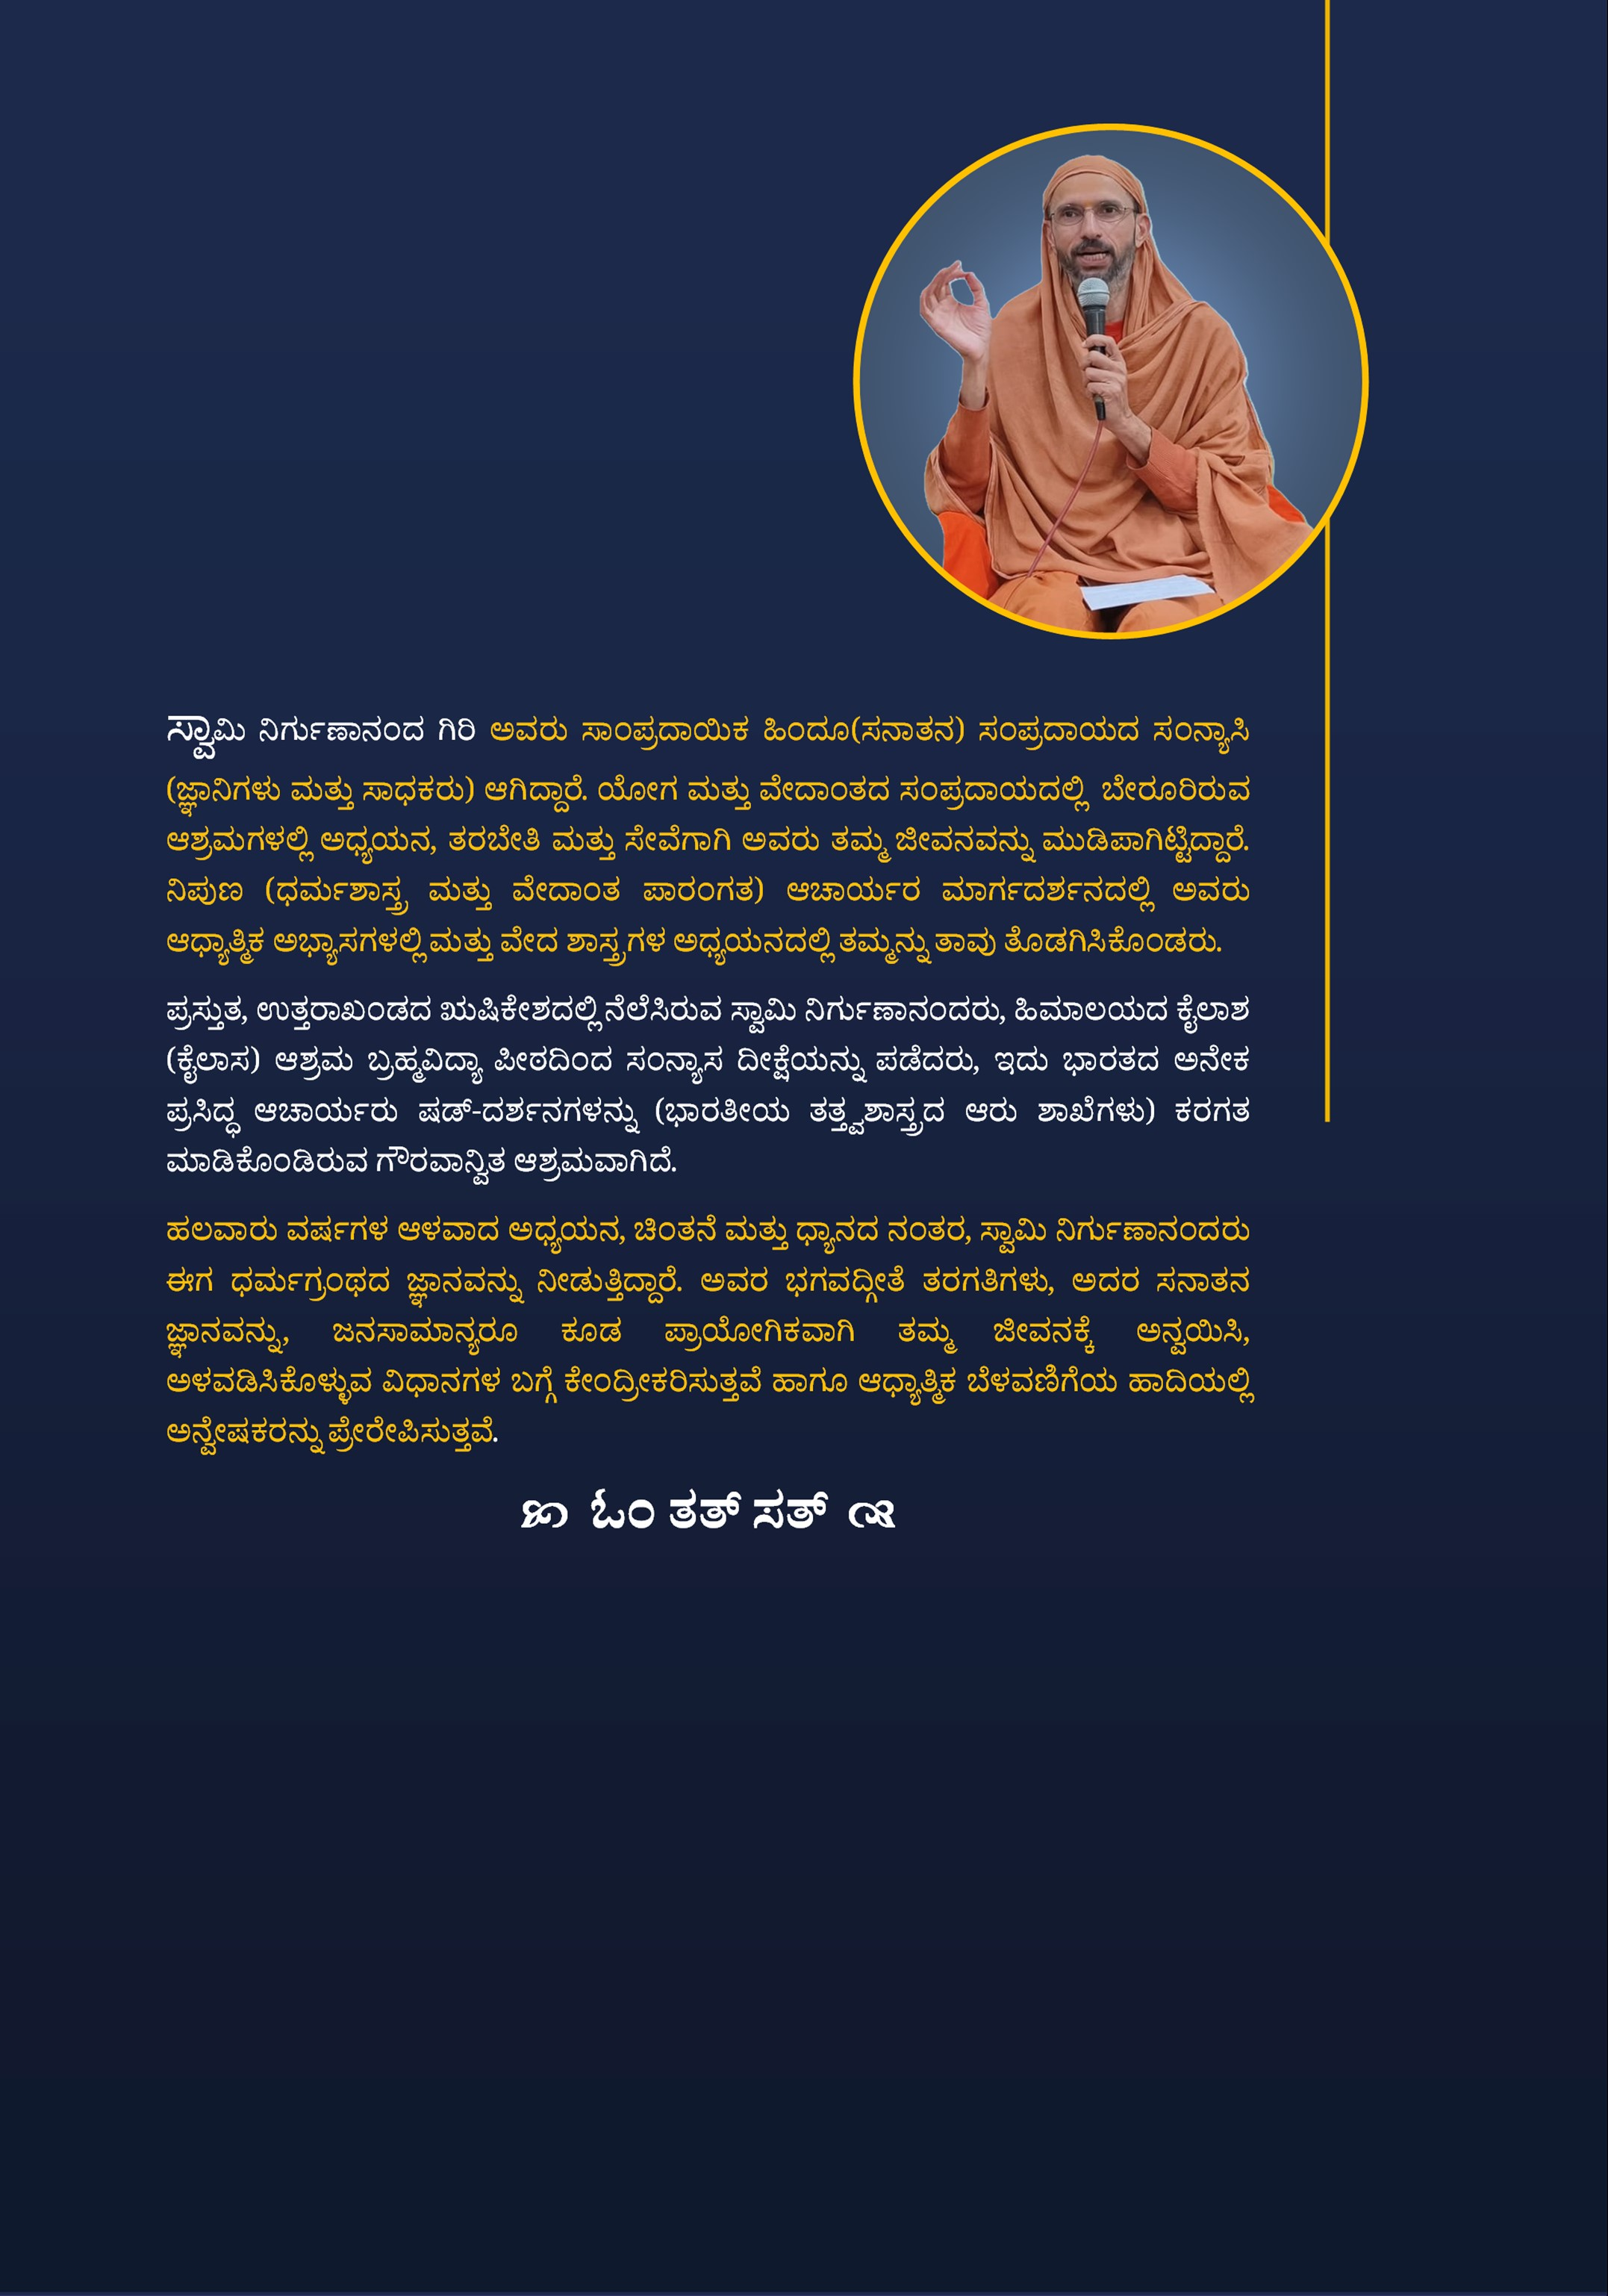
\includegraphics[width=\paperwidth,height=\paperheight]{./images/page02.jpg}%
    }%
	}
   \else% do nothing
   \AddToShipoutPictureBG*{%
    \AtPageLowerLeft{%
        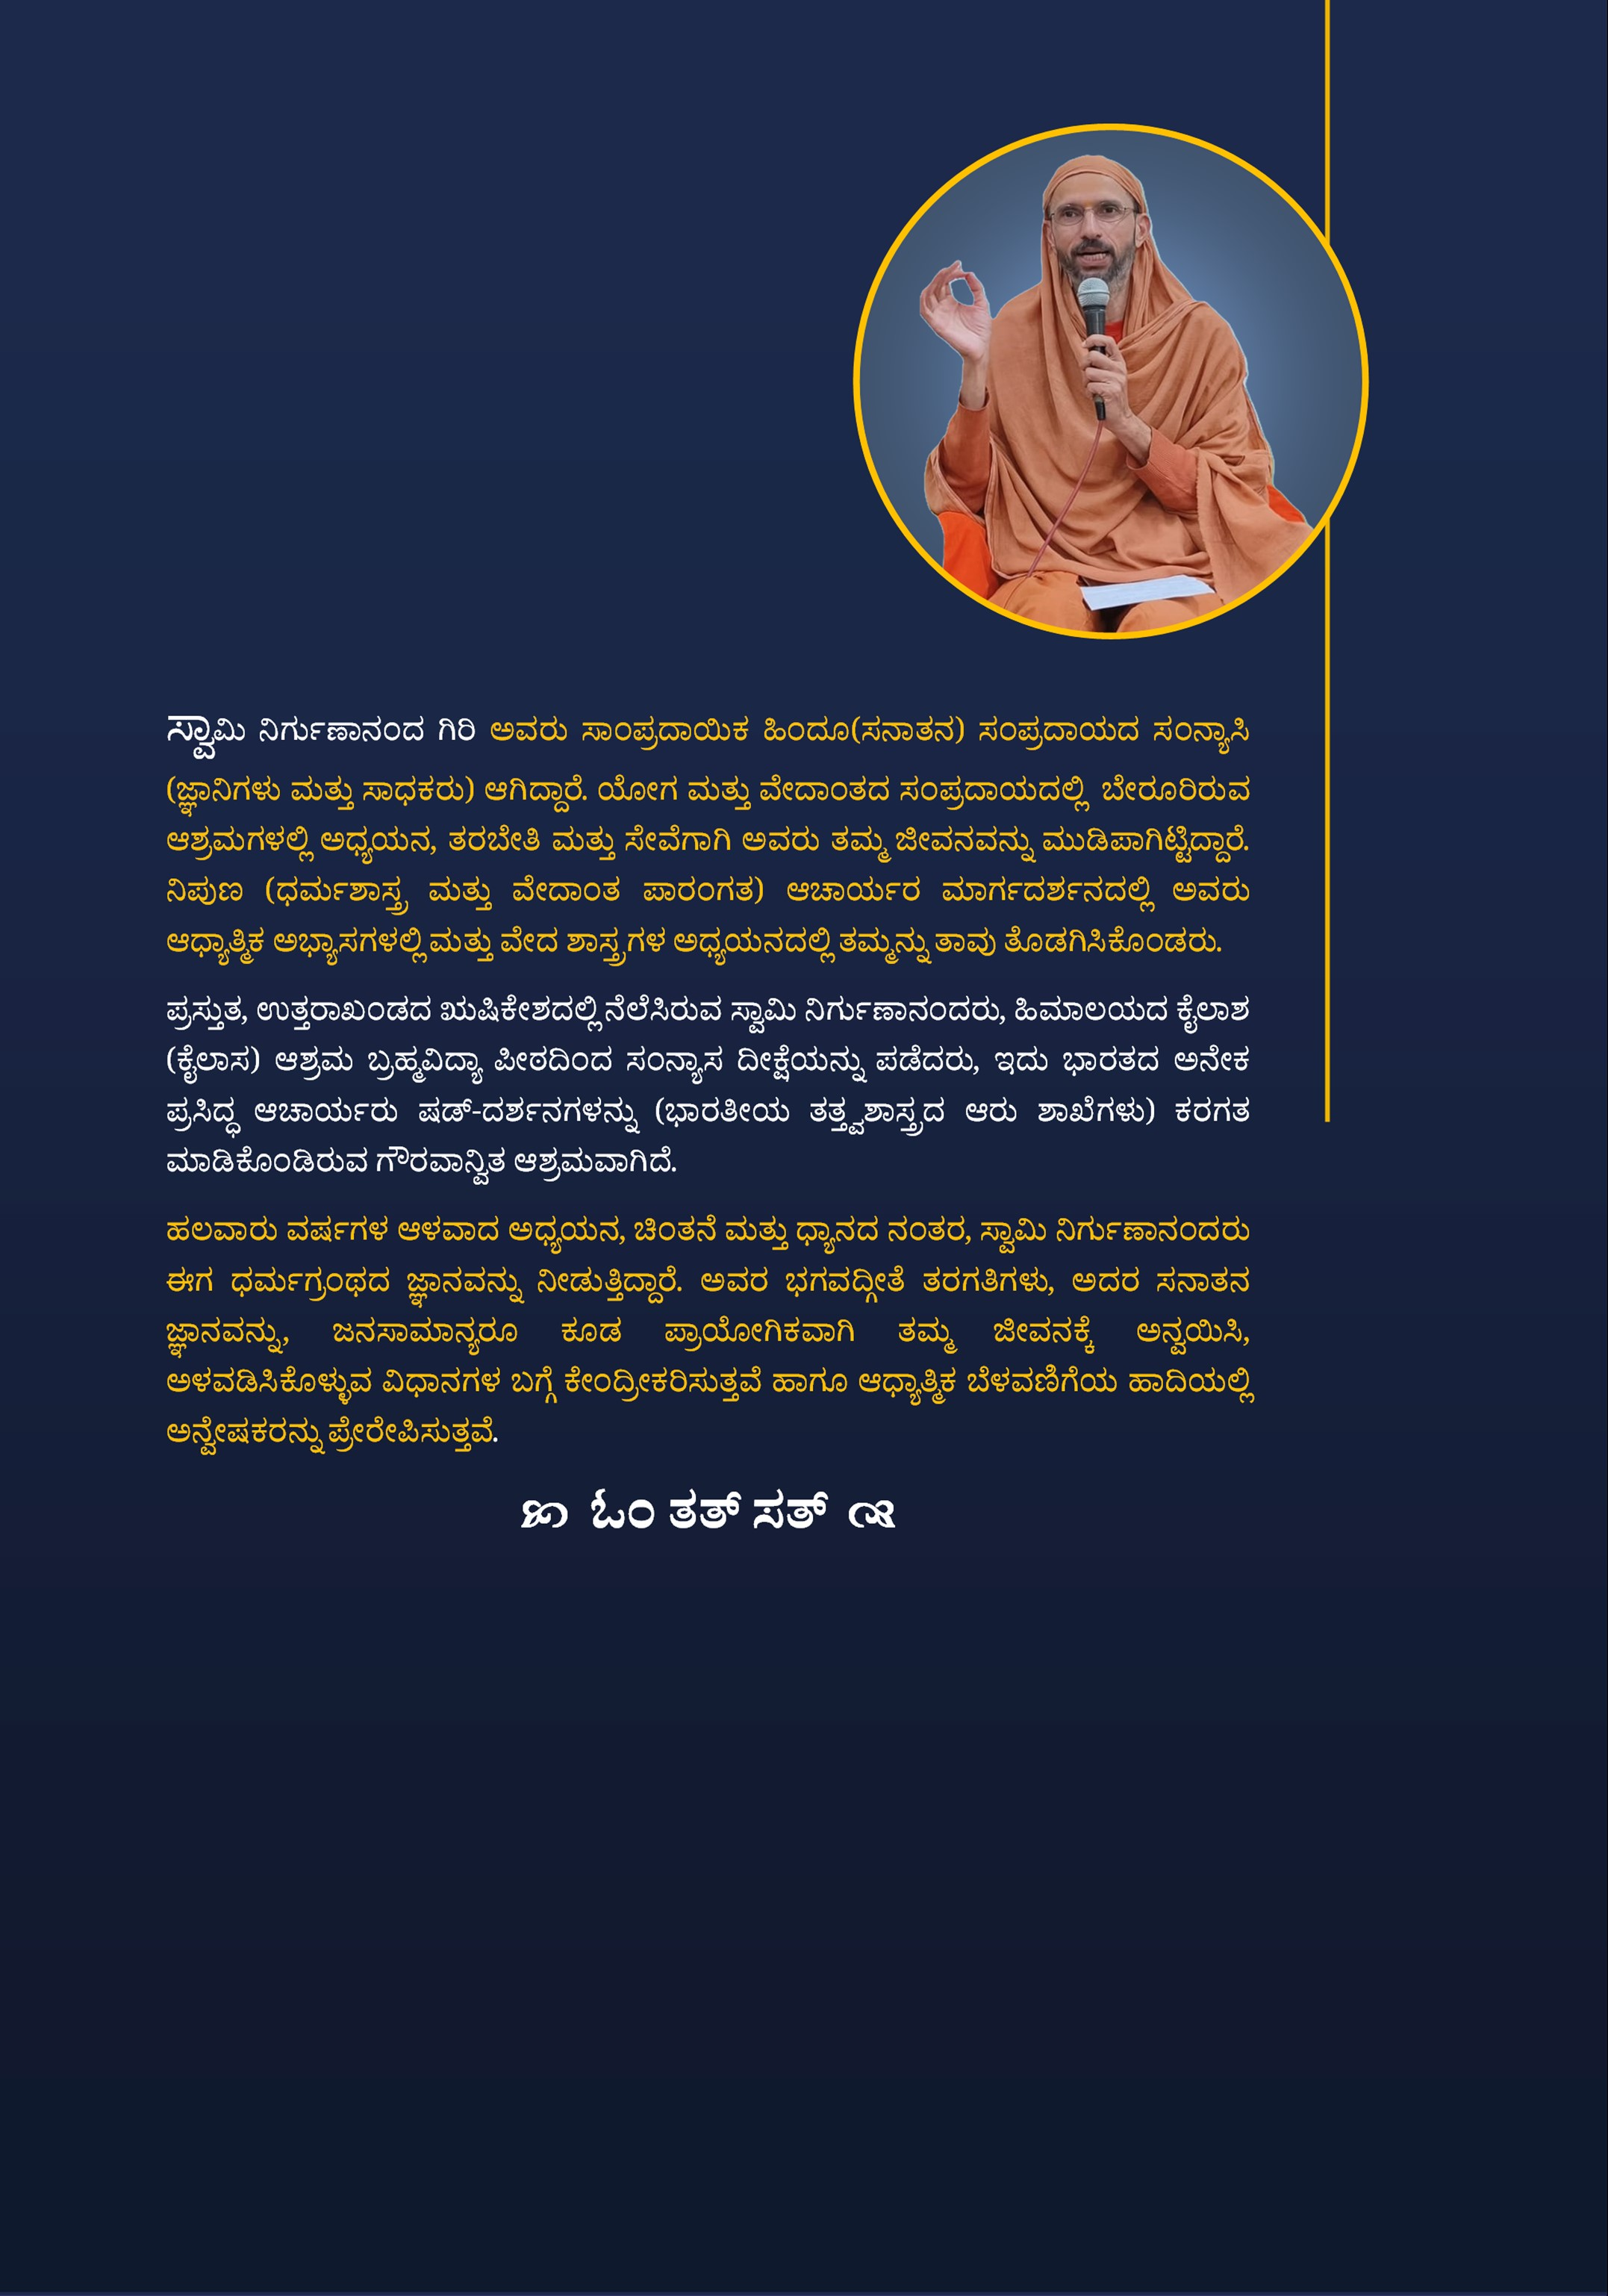
\includegraphics[width=\paperwidth,height=\paperheight]{./images/page02.jpg}%
    }%
	}
\fi
\begin{titlepage}
	%\pagecolor{pastelblue}
	\AddToShipoutPictureBG*{%
    \AtPageLowerLeft{%
        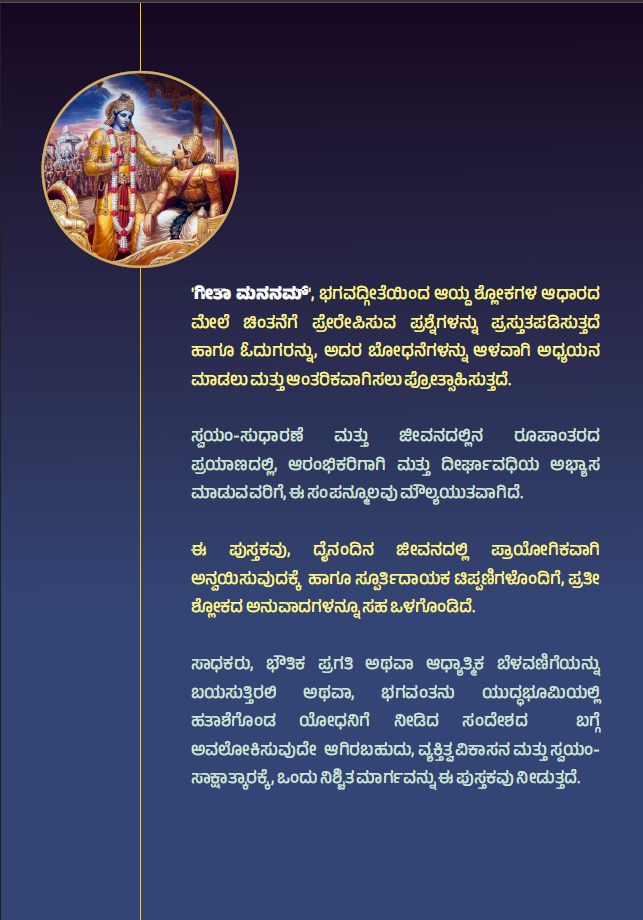
\includegraphics[width=\paperwidth,height=\paperheight]{./images/backcover.png}%
    }%
}
    \begin{center}
        \vspace*{0.5cm}
            
        {\Huge
        %\textbf{\color{white}\fontsize{50}{60}\selectfont ಗೀತಾ ಮನನಂ}
		}
        %\textbf{\\ \small \color{white}ದೈನಂದಿನ ಸ್ಪೂರ್ತಿ ಹಾಗೂ ಆತ್ಮಾವಲೋಕನಕ್ಕಾಗಿ}    
        \vspace{1.0cm}
            
        
		
            
        \vfill
            
        
            
        \vspace{0.1cm}
        {\color{white}    
		%\textbf{{\Large \mananamfont ಸ್ವಾಮಿ ನಿರ್ಗುಣಾನಂದ ಗಿರಿ}}\\
		%{\normalsize Swami Nirgunananda Giri\\Rishikesh, India}
        }
    \end{center}
\end{titlepage}
\nopagecolor% Use this to restore the color pages to white
\end{document}
